\section{Tight Forward Reasoning on Contract Compliance}

\paragraph{Methodological overview.}
This section develops the forward-looking semantics and monitoring constructions in a layered manner.
We first introduce tight satisfaction and violation as \emph{frontier-based} judgements over prefixes of a synchronous periodic trace.
These judgements identify the unique decisive point at which a contract becomes irrevocably satisfied or violated.
On top of this core semantics, we derive coarser verdicts, prove coherence properties, and construct Moore-style monitors that operationalize the semantics.
The continuation of this development extends the same methodology to responsibility-aware verdicts and blame monitoring.
\subsection{Denotational Semantics for Forward-Looking Tight Contract Satisfaction}\label{forwardsatsem}
Fix the tagged collaboration alphabet $\Sigma = \Sigma_C^{(1)} \cup \Sigma_C^{(2)}$
and the induced letter alphabet $\Gamma = 2^{\Sigma}$.
Traces, prefixes, suffixes, and their basic operators are as defined in
\ref{traces}.
In this subsection, we only introduce the forward-looking semantic
judgements used to evaluate contracts along such traces.

\medskip
\paragraph{Core tight judgements.}
All semantic clauses below are stated relative to the prefix structure
fixed in \ref{traces}.

We define two tight relations (inductively on the syntax of $C$):
\[
\pi\ \satt\ C \quad\text{(tight satisfaction)},\qquad
\pi\ \violt\ C \quad\text{(tight violation)}.
\]
Intuitively, $\satt$ holds exactly at the \emph{first prefix}
where the contract becomes satisfied (acceptance frontier),
and $\violt$ holds exactly at the \emph{first prefix}
where it becomes violated (rejection frontier).

\medskip
\paragraph{Derived judgements.}
Using these frontiers, we define the remaining derived relations of the five-valued semantics.
By Lemma~\ref{lem:mutual prefix}, at most one tight frontier can occur along a fixed trace, so the clauses below classify a prefix by its position relative to this (unique, if it exists) decisive point.

\begin{definition}[Post and Pre-satisfaction semantic definition]\label{def:postprecont}
For a contract $C$ and trace $\pi$ the Pre satisfaction relation $\presat$, the post satisfaction and violation relations, respectively $\postsat$ and $\postviol$ are defined on the structure of the trace $\pi$ and the tight satisfaction and violation relations:
\[
\begin{array}{rcl}
\pi\ \presat\ C
&\iff&
\forall\,k<|\pi|:\ \neg\big(\pi[1,k]\ \satt\ C\big)\ \nd\ \neg\big(\pi[1,k]\ \violt\ C\big),
\\[0.8ex]
\pi\ \postsat\ C
&\iff&
\exists\,k<|\pi|:\ \pi[1,k]\ \satt\ C,
\\[0.8ex]
\pi\ \postviol\ C
&\iff&
\exists\,k<|\pi|:\ \pi[1,k]\ \violt\ C.
\end{array}
\]
\end{definition}
Each trace prefix is classified relative to the earliest decisive prefix: before it the trace is undecided ($\presat$), at it the contract is decided tightly ($\satt$ or $\violt$), and after it the trace is beyond the decision frontier ($\postsat$ or $\postviol$).
The fact that these five regions are pairwise disjoint and jointly exhaustive is established formally in Theorem~\ref{thm:five-partition}.

\medskip
\paragraph{Collapsed two-valued judgements.}
For downstream use (e.g., compliance checking), we collapse the five tight judgements into a two-valued view.
For conservativeness, undecided prefixes are treated as violating, which prevents premature acceptance.
\[
\begin{array}{rcl}
\pi \models_\top \ C
&\iff&
\big(\pi\ \satt\ C\big)\ \sor\ \big(\pi\ \postsat\ C\big),
\\[0.6ex]
\pi\ \viol\ C
&\iff&
\big(\pi\ \presat\ C\big)\ \sor\ \big(\pi\ \violt\ C\big)\ \sor\ \big(\pi\ \postviol\ C\big).
\end{array}
\]
Exactly one of $\pi\ \sat\ C$ or $\pi\ \viol\ C$ holds for every trace~$\pi$ and contract~$C$.
This conservative collapse treats undecided prefixes as \emph{violating}
(no premature acceptance) while still preserving the tight moment of satisfaction.

\subsubsection*{Literal Tight Semantics}
Literals $\ell$ are decided in a single synchronous step.
We therefore interpret them on a single event word $\trace{A}$ with $A\in\Gamma$
(the set of actions that occurred in one period).

\par
We present the literal clauses for party $p=1$; the case $p=2$ is symmetric (by swapping $(\cdot)^{(1)}$ and $(\cdot)^{(2)}$).

Intuitively, for party~1:
(i) an \emph{obligation} $\obl[1]{a}$ requires the joint execution of $a^{(1)}$ and $a^{(2)}$;
(ii) a \emph{prohibition} $\frb[1]{a}$ is satisfied precisely when that joint execution does not occur; and
(iii) a \emph{power} $\perm[1]{a}$ requires that whenever party~1 attempts $a^{(1)}$,
party~2 simultaneously supports it with $a^{(2)}$.

%
\begin{definition}[Literal tight satisfaction]\label{def:lattsat}
  For the empty trace, we have:
  \[
  \emptytrace\ \presat \ell \quad \text{for any literal } \ell.
  \]
  Literals are decided on a single synchronous step. We define their semantics on a single event word $\trace{A}$ ($A\in\Gamma$) and the empty word $\emptytrace$.
  \[
  \emptytrace\ \presat \ell \quad \text{for any literal } \ell.
  \]
  \smallskip
  \noindent\textbf{Tight satisfaction.}
  For a single event word $\trace{A}$:
  \[
  \begin{array}{l@{\quad}c@{\quad}l}
  \trace{A}\ \satt\ \top      &\mydef& \text{true}.\\[4pt]
  \trace{A}\ \satt\ \bot      &\mydef& \text{false}.\\[6pt]
  \trace{A}\ \satt\ \obl[1]{a} &\mydef& \{a^{(1)},a^{(2)}\}\subseteq A.\\[6pt]
  \trace{A}\ \satt\ \frb[1]{a} &\mydef& \{a^{(1)},a^{(2)}\}\not\subseteq A.\\[6pt]
  \trace{A}\ \satt\ \perm[1]{a} &\mydef& \text{if }(a^{(1)}\in A) \text{ then }(a^{(2)}\in A).
  \end{array}
  \]
  
  \medskip
  
  \noindent\textbf{Tight violation.}
  For a single event word $\trace{A}$:
  \[
  \begin{array}{l@{\quad}c@{\quad}l}
  \trace{A}\ \violt\ \top      &\mydef& \text{false}.\\[4pt]
  \trace{A}\ \violt\ \bot      &\mydef& \text{true}.\\[6pt]
  \trace{A}\ \violt\ \obl[1]{a} &\mydef& \{a^{(1)},a^{(2)}\}\not\subseteq A.\\[6pt]
  \trace{A}\ \violt\ \frb[1]{a} &\mydef& \{a^{(1)},a^{(2)}\}\subseteq A.\\[6pt]
  \trace{A}\ \violt\ \perm[1]{a} &\mydef& (a^{(1)}\in A) \nd (a^{(2)}\notin A).
  \end{array}
  \]
  \end{definition}

\begin{example}[Literal satisfaction and violation]
Let $A=\{a^{(1)},a^{(2)},b^{(2)}\}$ be the joint actions in one period.
Then
\[
\trace{A}\ \satt\ \obl[1]{a},\qquad
\trace{A}\ \satt\ \perm[1]{a},\qquad
\trace{A}\ \satt\ \frb[2]{b}.
\]
Let $A'=\{a^{(1)},b^{(1)},b^{(2)}\}$. Then
\[
\trace{A'}\ \violt\ \perm[1]{a}\quad\text{(since $a^{(2)}\notin A'$)},\qquad
\trace{A'}\ \satt\ \frb[2]{a}\quad\text{(no joint $a^{(1)} \nd a^{(2)}$ occurs).}
\]
Also, $\trace{A'}\ \satt\ \perm[2]{a}$ holds vacuously since $a^{(2)}\notin A'$.

\medskip
\noindent\textbf{Two-event trace.}
Consider $\trace{A,A'}$.
Since literals are decided at the first letter,
the overall collapsed verdict follows from $\trace{A}$ are post satisfaction or post violation:
\[
\begin{array}{l}
\trace{A,A'}\ \postsat\ \obl[1]{a},\\[4pt]
\trace{A,A'}\ \postsat\ \perm[1]{a},\\[4pt]
\trace{A,A'}\ \postviol\ \perm[2]{b}.
\end{array}
\]
\end{example}

\subsubsection*{Binary Contract Operators Tight Semantics}
\label{sec:tight-binary}
Binary contract operators combine two contracts into structured compositions that capture
parallel, sequential, or conditional behavior.  
In \cDL\ we use
\[
\textsf{op} \in \{\wedge,\ ;\ ,\ \repair\},
\]
where $\wedge$ enforces \emph{both} components, $;$ demands \emph{first $C$ then $C'$},
and $\repair$ means “if $C$ fails, \emph{repair} with $C'$.”

\medskip
\noindent\textbf{Reading guide (tight view).}
All clauses below are tight: they identify the \emph{first decisive point}
where satisfaction or violation becomes determined.
For conjunction, the decisive point for satisfaction is the latter of the two individual successes; for violation, the first conjunct that fails.
For sequencing, a split index $k$ witnesses that $C$ succeeds before $C'$ is checked.
Reparation, on the other hand, requires that either $C$ succeeds directly, or, at the first tight violation of $C$, the repair $C'$ must succeed on the remainder.

\begin{definition}[Binary Contract Operators]
  \label{def:binary-contract-semantics}
  Let $\pi$ be a finite trace over $\Gamma = 2^{\Sigma}$ with  $s=\size{\pi}$.
  We use the notation $\pi_k = \pi[1,k]$ for the prefix of length $k$,
  and $\pi^k = \pi[k+1,s]$ for the suffix after $k$.

  \[
  \begin{array}{l@{\quad}c@{\quad}l}
  \multicolumn{3}{l}{\textbf{Conjunction }(C \wedge C')}\rule{0pt}{2.4ex}\\
  \pi\ \satt\ C \wedge C'
  &\mydef&
  \exists\,k,k' \in [1,s]:\
  \pi_{k}\ \satt\ C\ \nd\
  \pi_{k'}\ \satt\ C'\ \nd\ \\
  & &s=\max(k,k'),
  \\[1.2ex]
  \pi\ \violt\ C \wedge C'
  &\mydef&
  (\pi\ \violt\ C\ \sor\ \pi\ \violt\ C')\ \nd\ \\
  & &\forall\,j \in [1, s-1]:\ \lnot(\pi_{j}\ \violt\ (C \wedge C')),
  \\[2ex]

  \multicolumn{3}{l}{\textbf{Sequence }(C\ ;\ C')}\rule{0pt}{2.4ex}\\
  \pi\ \satt\ C ; C'
  &\mydef&
  \exists\,k \in [1, s-1]:\ \pi_k\ \satt\ C\ \nd\ \pi^{k}\ \satt\ C',
  \\[1.2ex]
  \pi\ \violt\ C ; C'
  &\mydef&
  \pi\ \violt\ C\ \sor\
  \exists\,k \in [1, s-1]:\ \pi_k\ \satt\ C\ \nd\ \pi^{k}\ \violt\ C',
  \\[2ex]

  \multicolumn{3}{l}{\textbf{Reparation }(C\ \repair\ C')}\rule{0pt}{2.4ex}\\
  \pi\ \satt\ C \repair C'
  &\mydef&
  \pi\ \satt\ C\ \sor\
  \exists\,k \in [1, s-1]:\ \pi_k\ \violt\ C\ \nd\ \pi^{k}\ \satt\ C',
  \\[1.2ex]
  \pi\ \violt\ C \repair C'
  &\mydef&
  \exists\,k \in [1, s-1]:\ \pi_k\ \violt\ C\ \nd\ \pi^{k}\ \violt\ C'.
  \end{array}
  \]
\end{definition}

\paragraph{Semantics summary.}
\emph{Conjunction} succeeds once both parts succeed (possibly at different times); its decisive index is the latter of the two.  
It fails as soon as either part fails.  
\emph{Sequence} requires a witness split $k$:
first $C$ succeeds on $[1,k]$, then $C'$ on $[k{+}1,s]$.
\emph{Reparation} allows $C'$ to take over at the first violation of $C$; overall success means either direct success of $C$
or a violation-then-repair pattern.


\begin{lemma}[Local disjointness of tight satisfaction and violation for binary operators]
  \label{lem:binary-disjoint}
  Let $C,C'$ be contracts and let $\pi$ be a finite trace. Assume the following
  induction hypotheses hold for the subcontracts:
  \[
  \neg\bigl(\pi \satt C \ \nd\ \pi \violt C\bigr)
  \qquad\text{and}\qquad
  \neg\bigl(\pi \satt C' \ \nd\ \pi \violt C'\bigr),
  \]
  and, moreover, the same disjointness holds for every suffix $\pi^{k}$ in place of $\pi$.
  Then, for each binary operator $\textsf{op}\in\{\wedge,\ ;\ ,\ \repair\}$ we have
  \[
  \neg\bigl(\pi \satt (C\ \textsf{op}\ C') \ \nd\ \pi \violt (C\ \textsf{op}\ C')\bigr).
  \]
  \end{lemma}
  
  \begin{proof}
    We prove the three cases by contradiction, using Definition~\ref{def:binary-contract-semantics}.
    We also use Lemma~\ref{lem:mutual prefix} to rule out an opposite frontier on a strict prefix once a tight verdict holds on the full trace.
    
    \paragraph{Case $\wedge$.}
    Assume $\pi \satt (C\wedge C')$ and $\pi \violt (C\wedge C')$.
    From $\pi \satt (C\wedge C')$ there exist $k,k'\in[1,s]$ such that
    $\pi_k \satt C$, $\pi_{k'} \satt C'$, and $s=\max(k,k')$.
    From $\pi \violt (C\wedge C')$ we obtain $\pi \violt C$ or $\pi \violt C'$.
    
    If $\pi \violt C$, then:
    (i) if $k=s$, we have $\pi \satt C$ and $\pi \violt C$, contradicting the disjointness hypothesis for $C$;
    (ii) if $k<s$, then $\pi_k$ is a strict prefix of $\pi$ with $\pi_k \satt C$, contradicting Lemma~\ref{lem:mutual prefix}(2) instantiated with $C$ (since $\pi \violt C$ forbids any $j<s$ with $\pi_j \satt C$).
    The case $\pi \violt C'$ is symmetric.
    
    \paragraph{Case $;$.}
    Assume $\pi \satt (C;C')$ and $\pi \violt (C;C')$.
    From satisfaction there exists $k\in[1,s-1]$ such that
    $\pi_k \satt C$ and $\pi^{k} \satt C'$.
    From violation either (i) $\pi \violt C$ or (ii) there exists $m\in[1,s-1]$ such that
    $\pi_m \satt C$ and $\pi^{m} \violt C'$.
    
    In case (i), $\pi \violt C$ contradicts Lemma~\ref{lem:mutual prefix}(2) for $C$
    because $\pi_k$ is a strict prefix with $\pi_k \satt C$.
    
    In case (ii), tight satisfaction of $C$ is a frontier event along prefixes of a fixed trace,
    so $\pi_k \satt C$ and $\pi_m \satt C$ imply $k=m$.
    Hence, the same suffix $\pi^{k}$ both tightly satisfies and tightly violates $C'$,
    namely $\pi^{k} \satt C'$ and $\pi^{k} \violt C'$,
    contradicting the suffix-disjointness hypothesis for $C'$.
    
    \paragraph{Case $\repair$.}
    Assume $\pi \satt (C\repair C')$ and $\pi \violt (C\repair C')$.
    From $\pi \violt (C\repair C')$ there exists $k\in[1,s-1]$ such that
    $\pi_k \violt C$ and $\pi^{k} \violt C'$.
    From $\pi \satt (C\repair C')$ either (a) $\pi \satt C$ or (b) there exists $m\in[1,s-1]$ such that
    $\pi_m \violt C$ and $\pi^{m} \satt C'$.
    
    In case (a), $\pi \satt C$ and the strict-prefix violation $\pi_k \violt C$ contradict
    Lemma~\ref{lem:mutual prefix}(1) instantiated with $C$.
    
    In case (b), tight violation of $C$ is also a frontier event along prefixes of a fixed trace,
    so $\pi_k \violt C$ and $\pi_m \violt C$ imply $k=m$.
    Hence, the same suffix $\pi^{k}$ both violates and satisfies $C'$,
    namely $\pi^{k} \violt C'$ and $\pi^{k} \satt C'$,
    contradicting the suffix-disjointness hypothesis for $C'$.
    
    Thus in all three cases we reach a contradiction, so
    $\neg\bigl(\pi \satt (C\ \textsf{op}\ C') \ \nd\ \pi \violt (C\ \textsf{op}\ C')\bigr)$.
    \end{proof}



\begin{example}[Tight satisfaction and violation for $(C_2 \wedge C_3)$]
\label{ex:c2c3-tight}
We reuse the collaboration alphabet
\[
\Sigma_C=\{\PAY,\ \PAYF,\ \OCC,\ \notifrepair,\ \REPAIR\},
\]
and recall
\[
C_2 := \perm[1]{\OCC}, \qquad
C_3 := \obl[1]{\PAY}\ \repair\ \obl[1]{\PAYF}.
\]

\paragraph{Tight satisfaction (the longest prefix).}
Consider the trace
\[
\pi_{\textsf{sat}} = \langle A_1, A_2\rangle,
\qquad
A_1=\{\OCC^{(2)}\},\quad
A_2=\{\PAYF^{(1)},\PAYF^{(2)}\}.
\]
Then
$\trace{A_1}\ \satt\ C_2$
(vacuously, since $\OCC^{(1)}\notin A_1$ and no unsupported attempt occurs),
and
$\pi_{\textsf{sat}}\ \satt\ C_3$
(the rent was not paid in month 1, but the reparation clause succeeds at $t{=}1$).
Hence, by conjunction,
$\pi_{\textsf{sat}}\ \satt\ (C_2 \wedge C_3)$
at the longest decisive prefix.

\paragraph{Tight satisfaction (the shortest prefix).}
For the single-event trace 
\[
\trace{A_1'} \quad\text{with}\quad A_1'=\{\OCC^{(2)},\PAY^{(1)},\PAY^{(2)}\},
\]
we have
$\trace{A_1'}\ \satt\ C_2$
and
$\trace{A_1'}\ \satt\ \obl[1]{\PAY}$,
so both conjuncts hold in month 1:
\[
\trace{A_1'}\ \satt\ (C_2 \wedge C_3),
\quad
\text{and any extension }\trace{A_1',A_2}\text{ yields }\postsat(C_2\wedge C_3).
\]

\paragraph{Tight violation.}
Now consider
\[
\pi_{\textsf{viol}} = \langle A_1, A_2\rangle,
\qquad
A_1=\{\OCC^{(1)}\},\quad
A_2=\emptyset.
\]
In the first month,
$\trace{A_1}\ \satt\ C_2$
and $\trace{A_1}\ \violt\ \obl[1]{\PAY}$,
while
$\trace{A_1}\ \presat\ C_3$
since the reparation in $C_3=\obl[1]{\PAY}\repair\obl[1]{\PAYF}$ has not yet been tested.
At $t{=}1$,
$\pi_{\textsf{viol}}\ \violt\ C_3$
(as $\pi[1,1]\ \violt\ \obl[1]{\PAY}$ and $\pi[2,2]\ \violt\ \obl[1]{\PAYF}$).
Thus, the overall violation arises from $C_3$,
and by conjunction,
$\pi_{\textsf{viol}}\ \violt\ (C_2 \wedge C_3)$.

\medskip
This shows that $(C_2 \wedge C_3)$
satisfies either immediately when both conjuncts hold, or later when a reparation compensates for a missed rent, while violation arises when both payment and its repair fail.
\end{example}

\subsubsection*{Repetition Contracts Tight Semantics}
\begin{definition}[Repetition Contracts]
  Let $\pi$ be a finite trace over the event alphabet $\Gamma = 2^{\Sigma}$, with $s=\size{\pi}$.
  For $k\in\{1,\dots,s-1\}$, we denote by $\pi_k := \pi[1,k]$ the prefix of length $k$,
  and by $\pi^k := \pi[k+1,s]$ the corresponding suffix.
  Let $n \in \mathbb{N}^*$ be a strictly positive natural number.
  
  The semantics for repetition contracts are inductively defined as follows:
  \[
  \begin{array}{lcl}
  \pi\ \satt\ C^n
  &\mydef& 
  \big( \text{if } n > 1 \text{ then } \pi\ \satt\ C ; C^{n-1} \big)\ \nd\ \big( n = 1 \Rightarrow \pi\ \satt\ C \big),
  \\[1.5ex]
  \pi\ \violt\ C^n
  &\mydef&
  \big(\pi\ \violt\ C\big)\ \sor\ \\ & &
  \big(\exists\,k\in[1,s-1],\exists\, 1 \le m < n:\\ & &\ \pi_k\ \satt\ C^m\ \nd\ \pi^{k}\ \violt\ C\big),
  \\[1.5ex]
  \pi\ \satt\ \repit{C}
  &\mydef&
  \text{false},
  \\[1ex]
  \pi\ \violt\ \repit{C}
  &\mydef&
  \exists\,n \in \mathbb{N}^*:\ \pi\ \violt\ C^n.
  \end{array}
  \]
\end{definition}
  
  \paragraph{Intuition.}
  Repetition contracts express the iterative enforcement of a subcontract.
  The finite form $C^n$ requires $C$ to hold $n$ times in sequence, each instance starting
  immediately after the previous one completes.
  The satisfaction condition unfolds recursively:
  a trace satisfies $C^n$ if it can be decomposed into a prefix where $C$ holds,
  followed by a suffix that satisfies $C^{n-1}$.
  A violation occurs either when the first occurrence of $C$ fails, or when some later repetition cannot be fulfilled after a previously satisfied segment (captured by the split $\pi_k \satt C^m$ and $\pi^{k} \violt C$).
  Hence, $C^n$ behaves as a \emph{sequential chain} of responsibilities and rights, and any broken link invalidates the entire chain.
  
  The infinite form $\repit{C}$ captures \emph{unbounded repetition}.
  Since finite traces cannot exhibit infinite iteration,
  $\repit{C}$ is never fully satisfied (\textsf{false} under tight semantics);
  it is only meaningful with respect to violation:
  a trace violates $\repit{C}$ once it violates one of its finite unfolding $C^n$.
  Intuitively, $\repit{C}$ models \emph{renewable or continuing} contracts such as
  subscriptions or recurring payments, where each cycle restarts the same normative
  condition indefinitely.

  % --- BEGIN INSERTED LEMMAS ---
\begin{lemma}[Local disjointness for repetition contracts]
  \label{lem:repetition-disjoint}
  Let $C$ be a contract, $n\in\mathbb{N}^*$, and let $\pi$ be a finite trace.
  Assume the induction hypothesis that for every finite trace $\Pi_{\min}$ we have
  $\neg(\Pi_{\min}\ \satt\ C\ \nd\ \Pi_{\min}\ \violt\ C)$, and moreover the same disjointness
  holds for every suffix $\Pi_{\min}^k$ in place of $\Pi_{\min}$.
  Then:
  \[
  \neg\bigl(\pi\ \satt\ C^n\ \nd\ \pi\ \violt\ C^n\bigr)
  \qquad\text{and}\qquad
  \neg\bigl(\pi\ \satt\ \repit{C}\ \nd\ \pi\ \violt\ \repit{C}\bigr).
  \]
  \end{lemma}
  
  \begin{proof}
  We prove the two claims.
  
  \paragraph{Finite repetition $C^n$.}
  We argue by induction on $n$.
  For $n=1$, we have $C^1\equiv C$ by definition, hence the claim follows from the hypothesis.
  For $n>1$, the definition gives $\pi\ \satt\ C^n$ iff $\pi\ \satt\ C;C^{n-1}$.
  Likewise, the violation clause for $C^n$ can only arise either from an initial violation of $C$,
  or after some satisfied prefix where a later copy of $C$ is violated.
  In either case, if we assume toward contradiction that
  $\pi\ \satt\ C^n$ and $\pi\ \violt\ C^n$, then we obtain a contradiction with
  (i) Lemma~\ref{lem:binary-disjoint} for the sequence operator (applied to $C$ and $C^{n-1}$),
  (ii) the induction hypothesis for $C$, and
  (iii) the induction hypothesis for $C^{n-1}$ together with the suffix-disjointness assumption.
  Thus, $\neg(\pi\ \satt\ C^n\ \nd\ \pi\ \violt\ C^n)$ holds.
  
  \paragraph{Unbounded repetition $\repit{C}$.}
  By definition, $\pi\ \satt\ \repit{C}$ is \emph{false} for every finite trace $\pi$.
  Hence, $\pi$ cannot both tightly satisfy and tightly violate $\repit{C}$.
  \end{proof}
  



  \subsubsection*{Regular Expression Binary Operator Semantics}
  \label{sec:regex-contract}
  Contracts guarded by regular expressions specify that a normative condition becomes active only after the trace matches a given regular pattern.  
  Such patterns, written $re$, are interpreted over the letter alphabet 
  $\Gamma = 2^{\Sigma}$ introduced above.  
  They act as \emph{temporal triggers} that delimit
  where an obligation, prohibition, or reparation clause starts to apply.
  
  Two guarded forms are distinguished:
  \begin{itemize}
    \item The \emph{triggered contract} $\trig[re]{C}$, which activates $C$ as soon as a prefix of the trace matches $re$.
    \item The \emph{guarded contract} $\guard[re]{C}$, which restricts $C$ to hold only while the trace remains within the language induced by $re$.
  \end{itemize}
  The first captures temporal activation (“after the trigger, $C$ must hold”),
  the second conditional persistence (“as long as $re$ remains possible, $C$ must hold”).
  
  \begin{definition}[Triggered and Guarded Contracts]
    \label{def:trigger-guard-semantics}
    Let $\pi$ be a finite trace over $\Gamma = 2^{\Sigma}$ with  $s=\size{\pi}$.
    \[
    \begin{array}{l@{\quad}c@{\quad}l}
    \pi\ \satt\ \trig[re]{C}
      &\mydef& 
      \pi\ \violt\ re\
      \sor\
      \big(\exists\,k \in [1, s-1]:\ \pi_k\ \satt\ re\ \nd\ \pi^{k}\ \satt\ C\big),
      \\[1.2ex]
    
      \pi\ \violt\ \trig[re]{C}
      &\mydef& 
      \exists\,k \in [1, s-1]:\ \pi_k\ \satt\ re\ \nd\ \pi^{k}\ \violt\ C,
      \\[2ex]
    
      \pi\ \satt\ \guard[re]{C}
      &\mydef&
      \big(\pi\ \violt\ re\ \nd\ \pi\ \clossat\ C\big)\
      \sor\
      \big(\pi\ \clossat\ re\ \nd\ \pi\ \satt\ C\big),
      \\[1.2ex]
    
      \pi\ \violt\ \guard[re]{C}
      &\mydef&
      \pi\ \clossat\ re\ \nd\ \pi\ \violt\ C.
    \end{array}
    \]
    Where $\pi\ \clossat\ X$ abbreviates $(\pi\ \presat\ X\ \sor\ \pi\ \satt\ X)$.
  \end{definition}
  
  \begin{lemma}[Local disjointness for triggered and guarded contracts]
    \label{lem:regex-disjoint}
    Let $re$ be a regular expression over $\Gamma$ and let $C$ be a contract.
    Assume disjointness for both components, namely for every finite trace $\Pi_{\min}$:
    \[
    \neg(\Pi_{\min}\ \satt\ re\ \nd\ \Pi_{\min}\ \violt\ re)
    \quad\text{and}\quad
    \neg(\Pi_{\min}\ \satt\ C\ \nd\ \Pi_{\min}\ \violt\ C),
    \]
    and assume the same disjointness holds for every suffix $\Pi_{\min}^k$ in place of $\Pi_{\min}$.
    Then for every finite trace $\pi$:
    \[
    \neg\bigl(\pi\ \satt\ \trig[re]{C}\ \nd\ \pi\ \violt\ \trig[re]{C}\bigr)
    \quad\text{and}\quad
    \neg\bigl(\pi\ \satt\ \guard[re]{C}\ \nd\ \pi\ \violt\ \guard[re]{C}\bigr).
    \]
  \end{lemma}
    
  \begin{proof}
    We treat the two constructors.
    
    \paragraph{Triggered $\trig[re]{C}$.}
    Assume toward contradiction that $\pi\ \satt\ \trig[re]{C}$ and $\pi\ \violt\ \trig[re]{C}$.
    From the violation clause, there exists $k \in [1, s-1]$ such that $\pi_k\ \satt\ re$ and $\pi^{k}\ \violt\ C$.
    
    From the satisfaction clause, either (a) $\pi\ \violt\ re$ or (b) there exists $m \in [1, s-1]$ such that $\pi_m\ \satt\ re$ and $\pi^{m}\ \satt\ C$.
    
    \noindent\emph{Case (a):} We have $\pi_k \satt re$ (from violation) and $\pi \violt re$ (from assumption).
    By Lemma~\ref{lem:mutual prefix} (Mutual Prefix Exclusion applied to $re$), if a prefix $\pi_k$ tightly satisfies $re$, the full trace $\pi$ (which is an extension of $\pi_k$) cannot tightly violate $re$. Contradiction.
    
    \noindent\emph{Case (b):} We have $\pi_k \satt re$ and $\pi_m \satt re$.
    By Lemma~\ref{lem:mutual prefix} applied to $re$, there is at most one prefix of $\pi$ that tightly satisfies $re$. Thus, $k=m$.
    This implies we have both $\pi^{k}\ \violt\ C$ and $\pi^{k}\ \satt\ C$ on the \emph{same} suffix.
    This contradicts the disjointness hypothesis for $C$ on the suffix $\pi^{k}$.
    
    Hence, $\pi$ cannot both tightly satisfy and tightly violate $\trig[re]{C}$.
    
    \paragraph{Guarded $\guard[re]{C}$.}
    Assume toward contradiction that $\pi\ \satt\ \guard[re]{C}$ and $\pi\ \violt\ \guard[re]{C}$.
    By Definition~\ref{def:trigger-guard-semantics}, violation means $\pi\ \clossat\ re$ and $\pi\ \violt\ C$.
    Satisfaction means either (i) $\pi\ \violt\ re$ and $\pi\ \clossat\ C$, or (ii) $\pi\ \clossat\ re$ and $\pi\ \satt\ C$.
    
    \noindent\emph{Case (ii):} This yields $\pi\ \clossat\ re$ (consistent) but $\pi\ \satt\ C$ and $\pi\ \violt\ C$. This contradicts the disjointness hypothesis for $C$.
    
    \noindent\emph{Case (i):} This yields $\pi\ \clossat\ re$ and $\pi\ \violt\ re$.
    Expanding $\clossat$, this means $(\pi\ \presat\ re \sor \pi\ \satt\ re) \nd \pi\ \violt\ re$.
    By the disjointness hypothesis for $re$, $\satt$ excludes $\violt$.
    By Lemma~\ref{lem:mutual prefix}, $\presat$ excludes $\violt$.
    Thus, Case (i) is impossible.
    
    Thus guarded contracts are also disjoint.
  \end{proof}

\begin{example}[Triggered and guarded contracts]
\label{ex:trigger-guard}
Let the collaboration alphabet be
\[
\Sigma_C=\{\PAY,\ \PAYF,\ \OCC,\ \notifrepair,\ \notifterm,\ \REPAIR\}.
\]

\paragraph{(a) Triggered contract.}
Clause~$C_4$ specifies that when the tenant requests a repair, the landlord must perform it within the following period:
\[
C_4 := \trig[\{\notifrepair^{(1)}\}]{\obl[2]{\REPAIR}}.
\]

\emph{Tight satisfaction.}
\[
\pi_{\mathsf{sat}}=\langle A_1,A_2\rangle,
\text{ with }
A_1=\{\notifrepair^{(1)}\} \nd
A_2=\{\REPAIR^{(1)},\REPAIR^{(2)}\}.
\]
In the first month, the trigger $\notifrepair^{(1)}$ occurs,
activating the repair obligation.
In month 2, the landlord performs $\REPAIR^{(1,2)}$,
thus $\pi_{\mathsf{sat}}\ \satt\ C_4$.

\emph{Tight violation.}
\[
\pi_{\mathsf{viol}}=\langle A_1,A_2'\rangle,
\text{ with }
A_1=\{\notifrepair^{(1)}\} \nd
A_2'=\emptyset.
\]
The trigger in month 1, but the obligation is unfulfilled:
$\pi_{\mathsf{viol}}\ \violt\ C_4$.

\paragraph{(b) Guarded repetition.}
To limit repetition to the occupancy period, combine guard and repetition:
\[
C_9 := \guard[\,\Gamma^+\,;\,\{\notifterm^{(1)}\}\,;\,\Gamma^{3}]{\repit{\obl[1]{\PAY}}}.
\]
The guard pattern 
$\Gamma^+;\{\notifterm^{(1)}\};\Gamma^{3}$
means “for any non-empty prefix up to the termination notice
$\notifterm^{(1)}$, and for at most three additional steps afterward.”
Within this region, the obligation to pay rent repeats.
Once $\notifterm^{(1)}$ occurs, the duty remains for three more periods,
and the contract is satisfied at $t{=}1{+}3{=}4$.

\emph{Tight satisfaction.}
\[
\pi_{\mathsf{sat}}=
\langle
A_1,A_2,A_3,A_4,A_5
\rangle,
\quad
\begin{array}{l}
A_1=\{\OCC^{(1)},\PAY^{(1)},\PAY^{(2)}\},\\
A_2=\{\notifterm^{(1)},\PAY^{(1)},\PAY^{(2)}\},\\
A_3=A_4=A_5=\{\PAY^{(1)},\PAY^{(2)}\}.
\end{array}
\]
The guard is satisfied in month 5 and the payments were all successful, hence $\pi_{\mathsf{sat}}\ \satt\ C_9$.

\emph{Tight violation.}
\[
\pi_{\mathsf{viol}}=
\langle
A_1,A_2,A_3,A_4,A_5
\rangle,
\quad
\begin{array}{l}
A_1=\{\OCC^{(1)},\PAY^{(1)},\PAY^{(2)}\},\\
A_2=\{\notifterm^{(1)},\PAY^{(1)},\PAY^{(2)}\},\\
A_3=\{\PAY^{(1)},\PAY^{(2)}\},\\
A_4=\emptyset,\\
A_5=\{\PAY^{(1)},\PAY^{(2)}\}.
\end{array}
\]
A missing payment in the fourth month breaks the repetition duty
while the guard still holds, so
$\pi_{\mathsf{viol}}\ \violt\ C_9$.
\end{example}

\subsubsection*{Coherence of the Forward-Looking Contract Satisfaction Semantics}

Coherence requires that for any fixed contract and trace, there is never more than one decisive verdict. A trace cannot both tightly satisfy and tightly violate the same contract on different prefixes, since this would yield two incompatible outcomes for a single execution. Forward semantics must therefore
rule out situations where tight satisfaction appears on one prefix and tight violation appears on another prefix of the same trace. Ensuring this exclusion
makes the decisive point unique, which is required to justify every verdict from $\tightverdicts$.
The next lemma states this exclusion precisely by showing that the two frontiers cannot arise on distinct prefixes of the same trace.

\begin{lemma}[Mutual prefix exclusion tight satisfaction and violation]
\label{lem:mutual prefix}
For every contract $C$ in \cDL\ and every finite trace $\pi$, the tight satisfaction and tight violation forward semantics are mutually exclusive, that is:
\begin{enumerate}
  \item \emph{No earlier tight violation at or after tight satisfaction.}\\[2pt]
   $\text {If }\displaystyle \pi\ \satt\ C \ \text{then}\ \nexists\,j<|\pi|:\ \pi[1,j]\ \violt\ C\big.$

  \item \emph{No earlier tight satisfaction at or after tight violation.}\\[2pt]
  $\displaystyle \text {if } \pi\ \violt\ C \ \text{then}\ \nexists\,j<|\pi|:\ \pi[1,j]\ \satt\ C\big.$
\end{enumerate}


\end{lemma}

\begin{proof}[Proof sketch]
By structural induction on the syntactical structure of $C$.

\smallskip
\emph{Base case: literals.}
By Definition~\ref{def:lattsat}, a literal is decided on a single letter:
$\trace{A}\ \satt\ \ell$ iff the letter constraint holds, and
$\trace{A}\ \violt\ \ell$ iff it does not. These are complements on that step, so the two implications are immediate, and uniqueness follows.

\medskip
\noindent\textbf{Inductive hypotheses.}
Assume the theorem holds for subcontracts as needed below. We use:
\[
\begin{aligned}
\text{(IH-$C$-sat)}\quad 
&\forall\pi\; \bigl(\pi\ \satt\ C \Rightarrow \forall j<|\pi|:\neg(\pi[1,j]\ \violt\ C)\bigr),\\
\text{(IH-$C$-viol)}\quad 
&\forall\pi\; \bigl(\pi\ \violt\ C \Rightarrow \forall j<|\pi|:\neg(\pi[1,j]\ \satt\ C)\bigr),
\end{aligned}
\]
and similarly (IH-$C'$-sat) and (IH-$C'$-viol) when a second operand $C'$ is present; for regex guards $re$ we use the same two clauses with $re$ in place of $C$.

\paragraph{Conjunction $C\wedge C'$.}
By Definition~\ref{def:binary-contract-semantics}, tight satisfaction requires
first successes at some $k,k'$ with decisive index $j^\star=\max\{k,k'\}$.
For every $j<j^\star$, either $j<k$ or $j<k'$ holds, hence by (IH-$C$-sat) and
(IH-$C'$-sat) neither $\pi[1,j]\ \violt\ C$ nor $\pi[1,j]\ \violt\ C'$ holds.
Since a tight violation of a conjunction is a tight violation of the conjunction,
no $j<j^\star$ violates $C\wedge C'$. This proves the first implication.
For the second, if some prefix tightly violates a conjunct, then by
(IH-$C$-viol) or (IH-$C'$-viol) no earlier prefix tightly satisfies that conjunct, hence, no earlier prefix tightly satisfies the conjunction.

\paragraph{Sequence $C;C'$.}
By Definition~\ref{def:binary-contract-semantics}, tight satisfaction needs a split
$k$ with $\pi[1,k]\ \satt\ C$ and $\pi[k{+}1,|\pi|]\ \satt\ C'$.
For any $j\le k$, (IH-$C$-sat) forbids $\pi[1,j]\ \violt\ C$; for any
$j>k$, (IH-$C'$-sat) applied to the suffix forbids $\violt C'$ before its
own decisive point. A tight violation of $C;C'$ before satisfaction is either
a violation of $C$ before $k$ or a violation of $C'$ after $k$, both excluded.
The dual implication follows from (IH-$C$-viol) and (IH-$C'$-viol).

\paragraph{Reparation $C\repair C'$.}
By Definition~\ref{def:binary-contract-semantics}, either $C$ succeeds, or else at
the first tight violation index $k$ of $C$ the repair $C'$ must succeed on
$\pi^{k}$. In the first branch (IH-$C$-sat), it excludes earlier violations.
In the second branch, (IH-$C$-viol) gives minimal property of the failure point of $C$,
and (IH-$C'$-sat) on the suffix excludes earlier failure of the composite
before its tight success. The dual implication is symmetric, using (IH-$C$-viol) and (IH-$C'$-viol).

\paragraph{Finite repetition $C^n$.}
Unfold $C^n \equiv C;(C^{n-1})$ and argue by a secondary induction on $n$,
using the sequence case and the induction hypotheses for $C$ and $C^{n-1}$.

\paragraph{Unbounded repetition $\repit{C}$.}
Under tight semantics $\repit{C}$ never tightly satisfies and tightly violates
iff some finite unrolling $C^m$ tightly violates. The two implications reduce
to the finite case above.

\paragraph{Triggered $\langle re\rangle C$.}
By Definition~\ref{def:trigger-guard-semantics}, either $re$ is violated and the
contract tightly satisfies vacuously, or there is a first $k$ with $\pi_k\ \satt\ re$
and then the suffix must satisfy $C$. In the vacuous branch,
(IH-$re$-viol) forbids any earlier tight satisfaction of $re$, so there is no
earlier tight violation of the composite. In the active branch, the first match
index $k$ is minimal by (IH-$re$-sat); before $k$ the composite is undecided, and
after $k$ we apply (IH-$C$-sat)/(IH-$C$-viol) on the suffix to obtain both implications.

\paragraph{Guarded $[re]\,C$.}
While $\pi$ \emph{closes} $re$ (that is, $\pi$ is in the open region for $re$), any tight or post failure of $C$ yields a tight or post failure of the composite.
Once $re$ becomes impossible, the composite satisfies provided $C$ has not failed.
Combine (IH-$re$-sat) and (IH-$re$-viol) with (IH-$C$-sat) and (IH-$C$-viol),
and the guarded case table in Definition~\ref{def:trigger-guard-semantics}, to derive the two implications.

\medskip
All constructors preserve the two “no-backtrack” properties; hence, the claim holds for all $C$.
\end{proof}


% --- BEGIN INSERTED LEMMA ---
\begin{lemma}[Constructor-wise disjointness of the tight frontiers]
\label{lem:constructor-disjoint}
For every contract $C$ in \cDL\ and every finite trace $\pi$, we have
\[
\neg\bigl(\pi\ \satt\ C\ \nd\ \pi\ \violt\ C\bigr).
\]
\end{lemma}

\begin{proof}
By structural induction on the syntax of $C$.

\emph{Base: literals.} Disjointedness holds by Definition~\ref{def:lattsat}, since on a single letter the satisfaction and violation clauses are complementary.

\emph{Inductive steps.}
For binary constructors $C_1\wedge C_2$, $C_1;C_2$, and $C_1\repair C_2$, the claim follows from Lemma~\ref{lem:binary-disjoint} and the induction hypotheses for $C_1$ and $C_2$ (including the required suffix form).
For repetition constructors $D^n$ and $\repit{D}$, the claim follows from Lemma~\ref{lem:repetition-disjoint} and the induction hypothesis for $D$.
For triggered and guarded constructors $\trig[re]{D}$ and $\guard[re]{D}$, the claim follows from Lemma~\ref{lem:regex-disjoint} together with the induction hypotheses for $re$ and $D$.
No other constructors exist.
\end{proof}
% --- END INSERTED LEMMA ---

\begin{theorem}[Consistency of the forward-looking five tight semantics for \cDL]\label{thm:five-partition}
The five forward satisfaction relations
$\{\presat,\satt,\violt,\postsat,\postviol\}$ for \cDL are pairwise disjoint and jointly exhaustive.
\end{theorem}
\begin{proof}
Fix a finite trace $\pi$ and contract $C$.
We reason point-wise on prefixes of $\pi$ (as defined in Section~\ref{traces}) and lift the result to the trace-level relations via Definition~\ref{def:postprecont}.

By Lemma~\ref{lem:mutual prefix}, along a fixed trace the two frontiers cannot both occur on (possibly different) prefixes: if some prefix tightly satisfies $C$, then no prefix tightly violates $C$, and conversely.
Moreover, constructor-wise disjointness holds point wise for every prefix, that is, $\neg(\Pi_{\min}\ \satt\ C\ \nd\ \Pi_{\min}\ \violt\ C)$ for every prefix $\Pi_{\min}$.
This is established formally in Lemma~\ref{lem:constructor-disjoint}.

Now consider any prefix position $j$ with $1\le j<|\pi|$ and view the corresponding trace prefix $\pi[1,j]$.
By Definition~\ref{def:postprecont}, for a given prefix $\Pi_{\min}:=\pi[1,j]$ exactly one of the following holds:
(i) $\Pi_{\min}\ \presat\ C$ (no earlier prefix of $\Pi_{\min}$ is decisive),
(ii) $\Pi_{\min}\ \satt\ C$,
(iii) $\Pi_{\min}\ \violt\ C$,
(iv) $\Pi_{\min}\ \postsat\ C$ (some earlier prefix of $\Pi_{\min}$ tightly satisfies $C$), or
(v) $\Pi_{\min}\ \postviol\ C$ (some earlier prefix of $\Pi_{\min}$ tightly violates $C$).
These cases are mutually exclusive by the local disjointness results above together with Lemma~\ref{lem:mutual prefix}, which prevents mixing satisfaction-frontiers and violation-frontiers along the same trace.

Therefore, the five relations $\{\presat,\satt,\violt,\postsat,\postviol\}$ are pairwise disjoint and jointly exhaustive on prefixes of $\pi$.
Since $\pi$ was arbitrary, the claim holds for all finite traces.
\end{proof}




\paragraph{Next step.}
After establishing the forward tight satisfaction semantics in \cDL and studied their soundness. We now move from the denotational clauses to an operational view:  we construct the corresponding Moore-style monitors for the tight five-valued semantics and establish that their outputs coincide with the semantic judgements on every finite trace prefix.


\subsection{Monitor Construction for Tight Contract Satisfaction}

In the previous section, we established the mathematical rules that define exactly when a contract is satisfied or violated. 
Now, we turn those abstract definitions into an operational implementation: a finite-state monitor that tracks compliance step-by-step as events occur. 
We design these as Moore-style machines, which means the monitor maintains a running summary of the interaction; every state corresponds directly to one of the five possible verdicts (such as "tight satisfaction" or "undecided"). By ensuring these monitors update deterministically with every new event, we create a reliable, automated way to check compliance that matches our theoretical rules perfectly.
\begin{definition}[Moore machine on tight satisfaction verdicts]
    \label{def:tightsatmon}
    The \emph{Moore machine on tight satisfaction verdicts}, written $\tmon$, is a Moore machine whose output alphabet is the five-valued verdict set $\tightverdicts$.
    That is:
    \[
    \tmon = (Q,q_0,\Gamma,\tightverdicts,\delta,\lambda_{5}),
    \]
    where:
    \begin{enumerate}
    \item The output alphabet formed by 5 letters is 
    \[
    \tightverdicts = \{\mathsf{?},\topt,\bott,\topp,\botp\}.
    \]
    \item $Q$ is the set of states and $q_0\in Q$ is the initial state,
    \item $\Gamma$ is the input event alphabet,
    \item $\delta: Q \times \Gamma \to Q$ is the transition function,
    \item $\lambda_{5}: Q \to \tightverdicts$ is the state output function.
    \end{enumerate}
    \end{definition}

The next definition introduces the construction for any contract into its tight
satisfaction monitor. The construction is a function that maps each contract $C$ to a tight satisfaction monitor that enforces it. The construction proceeds by structural induction on the syntax of $C$, and each operator in \cDL is matched by a corresponding monitor combination operator. Regular expression guards and triggers rely on the
tight satisfaction monitor $\tsmc(\re)$ introduced earlier in
Definition~\ref{def:tsmc-re}.

\begin{definition}[Tight Satisfaction Monitor Construction]
 \label{def:tsmc}
The \emph{tight satisfaction monitor construction} is a function defined on $\cDL$, written  $\tsmc(C)$, that returns the tight satisfaction monitor for a contract
$C$ in \cDL. It is defined inductively on the structure of $C$:
 \[
\tsmc(C) \;:=\;
\begin{cases}
  \tsmc_{\mathit{lit}}(\ell)
    & \text{if } C = \ell, \\[0.4em]

  \tsmc_{\mathit{\wedge}}\big(\tsmc(C_1),\tsmc(C_2)\big)
    & \text{if } C = C_1 \wedge C_2, \\[0.4em]

  \tsmc_{\mathit{;}}\big(\tsmc(C_1),\tsmc(C_2)\big)
    & \text{if } C = C_1 ; C_2, \\[0.4em]

  \tsmc_{\mathit{\repair}}\big(\tsmc(C_1),\tsmc(C_2)\big)
    & \text{if } C = C_1 \repair C_2, \\[0.4em]

  \tsmc_{\trigg}(\re,C')
    & \text{if } C = \trig[\re]{C'}, \\[0.4em]

  \tsmc_{\guardd}(\re,C')
    & \text{if } C = \guard[\re]{C'}, \\[0.4em]

  \tsmc_{\mathit{nrep}}\big(n,\tsmc(C')\big)
    & \text{if } C = (C')^n, \\[0.4em]

  \tsmc_{\mathit{Rep}}\big(\tsmc(C')\big)
    & \text{if } C = \repit{C'}\;.
\end{cases}
\]
Where the tight monitor construction for regular expressions $\tsmc(\re)$ is already defined in Definition~\ref{def:tsmc-re}.
\end{definition}

\paragraph{Monitor correctness invariant.}
The monitor construction preserves the following invariant.
For every contract $C$ in \cDL, every finite trace $\pi$, and every prefix $\pi_k$,
the state reached by the monitor $\tsmc(C)$ after reading $\pi_k$
emits exactly the verdict prescribed by the five-valued tight semantics, that is:
\[
\lambda_5\bigl(\delta(q_0,\pi_k)\bigr) \;=\; \semfive{\pi_k \vDash C}.
\]
All operator-specific constructions are designed to preserve this invariant under
synchronous product, redirection, and state elimination.
Correctness lemmas below establish that the invariant holds inductively for each
contract constructor. 

We construct in the next subsections the tight satisfaction monitors compositionally from the syntax of contracts.
The construction proceeds by structural induction on the contract and associates to each
contract operator a corresponding monitor-combination operator.
Conceptually, this follows the classical construction paradigm of Thompson for regular expressions,
where complex behaviors are obtained by composing simpler automata.
However, rather than constructing an intermediate nondeterministic automaton and determinizing it afterward,
we perform the construction directly at the level of deterministic Moore machines.
In particular, verdict propagation is built into the states and outputs of the monitor from the outset,
so that tight satisfaction and violation are observed incrementally on prefixes of the trace.
This avoids a separate determinization step and ensures that the monitor semantics coincides
by construction with the five-valued tight semantics.

\subsubsection*{Construction for Literal Contracts}
\paragraph{From Tight Semantics to 5-Valued Monitoring.}
The literal clauses above define one-step satisfaction and violation judgements for a single event word $\trace{A}$.
We lift these clauses into a five-valued Moore machine whose outputs track the evolution of the tight verdicts over prefixes.
\begin{definition}[Tight Satisfaction Monitor Construction for Literals]
\label{def:moore-5-literal}
For a literal $\ell$ from \cDL, the \emph{Tight Satisfaction monitor construction} for $\ell$, written $\tsmc_{\mathit{lit}}(\ell)$ is defined as:
\[
\tsmc_{\mathit{lit}}(\ell)
  = (Q, q_0, \Gamma, \tightverdicts, \delta, \lambda_5).
\]
\begin{itemize}
  \item $Q=\{q_0,q_s,q_v,q_{ps},q_{pv}\}$,
        with outputs
        $\lambda_5(q_0)=\mathsf{?}$,
        $\lambda_5(q_s)=\topt$,
        $\lambda_5(q_v)=\bott$,\\
        $\lambda_5(q_{ps})=\topp$,
        $\lambda_5(q_{pv})=\botp$.
  \item $\Gamma=2^{\Sigma}$ is the event alphabet.
  \item $\delta:Q\times\Gamma\to Q$ is defined as follows:
\[
\begin{aligned}
&\text{(1) tight transition: } 
&& \delta(q_0,A)=
  \begin{cases}
    q_s & \text{if }\trace{A}\ \satt\ \ell,\\
    q_v & \text{if }\trace{A}\ \violt\ \ell;
  \end{cases}\\[2pt]
&\text{(2) post transitions: }
&& \delta(q_s,A)=q_{ps},\ \delta(q_v,A)=q_{pv},\ \\ & &&
   \delta(q_{ps},A)=q_{ps},\ \delta(q_{pv},A)=q_{pv}.
\end{aligned}
\]

\end{itemize}
\end{definition}

\paragraph{Intuition.} For every atomic literal, the monitor construction initializes at $q_0$, emitting the undecided verdict $\mathsf{?}$ to reflect the absence of decisive information.
Upon consuming the first event, the execution crosses the decisive frontier, transitioning to either $q_s$ (success at frontier) with verdict $\topt$ if the literal is satisfied, or $q_v$ (violation at frontier) with verdict $\bott$ if it is violated.
On the next step after this decision, the monitor enters the stable regions $q_{ps}$ (post-success) or $q_{pv}$ (post-violation), where it permanently emits $\topp$ or $\botp$ respectively.
These indices explicitly encode the temporal relationship to the frontier, distinguishing the exact moment of decision from the immutable history of the trace.

\begin{figure}[h!]
\centering
\begin{tikzpicture}[
shorten >=1pt,auto,node distance=28mm,semithick,
  every state/.style={rectangle,rounded corners,draw,minimum width=11mm,
    minimum height=7.5mm,inner sep=5pt,font=\footnotesize,align=center}
]

% --- states ---------------------------------------------------
\node[initial,state,fill=gray!10] (q0)  {$q_0$\\[0.2pt]$\mathsf{?}$};
\node[state,fill=green!18,right=of q0] (qs)  {$q_s$\\[0.2pt]$\topt$};
\node[state,fill=red!18,below=of q0]   (qv)  {$q_v$\\[0.2pt]$\bott$};
\node[state,fill=green!10,right=of qs] (qps) {$q_{ps}$\\[0.2pt]$\topp$};
\node[state,fill=red!10,below=of qps]  (qpv) {$q_{pv}$\\[0.2pt]$\botp$};

% --- transitions ----------------------------------------------
\path[->]
  (q0) edge[bend left=12] node[above,pos=0.5]
    {$\{a^{(1)},a^{(2)}\}\subseteq A$} (qs)
  (q0) edge[bend right=12] node[left,pos=0.45]
    {$\{a^{(1)},a^{(2)}\} \not\subseteq A$} (qv)
  (qs)  edge node[above] {$\Gamma$} (qps)
  (qv)  edge node[below] {$\Gamma$} (qpv)
  (qps) edge[loop right] node {$\Gamma$} (qps)
  (qpv) edge[loop right] node {$\Gamma$} (qpv);
\end{tikzpicture}
\caption{Compact 5-verdict Moore machine for the obligation literal
$\obl[1]{a}$. 
Each node displays its internal state and the corresponding output verdict $\in\tightverdicts$.
The first joint execution of $a^{(1)}$ and $a^{(2)}$ yields~$\topt$,
otherwise~$\bott$; subsequent steps emit the post-frontier verdicts
$\topp$ or $\botp$.}
\label{fig:moore-obligation-compact}
\end{figure}


\subsubsection*{Construction for Binary Contract Operators}

For binary contract operators of the form $C\ \textsf{op}\ C'$ with
$\textsf{op} \in \{\wedge,\ ;\ ,\ \repair\}$, the monitor for the composite contract is obtained by combining the already constructed monitors
$\tsmc(C)$ and $\tsmc(C')$. Each operator has its own monitor construction,
defined below for conjunction, sequence, and reparation. We begin with the
conjunction case.


\begin{definition}[Tight Satisfaction Monitor Construction for Conjunction]
\label{def:moore-5-conj}
Let $C$ and $C'$ be contracts in \cDL, and let
\[
\tsmc(C)  = (Q, q_0, \Gamma, \tightverdicts, \delta, \lambda_5)
\quad\text{and}\quad
\tsmc(C') = (Q', q'_0, \Gamma, \tightverdicts, \delta', \lambda'_5).
\]
The tight satisfaction monitor construction for the conjunction
$C \wedge C'$, written $\tsmc_{\wedge}(C,C')$, is defined as:
\[
\tsmc_{\wedge}(C,C')
  = (Q_{\wedge}, q_0^{\wedge}, \Gamma, \tightverdicts, \delta_{\wedge}, \lambda_5^{\wedge}).
\]

\begin{itemize}
  \item The state set is the Cartesian product
  \[
    Q_{\wedge} = Q \times Q',
  \]
  with the initial state
  \[
    q_0^{\wedge} = (q_0,\,q'_0).
  \]

  \item The output function is
  \[
    \lambda_5^{\wedge}(x,y) =
    \lambda_{5}^{\textsf{comb}}\!\big(\lambda_5(x),\ \lambda'_5(y)\big),
  \]
  where $\lambda_{5}^{\textsf{comb}}$ is the conjunction-combination table:
  \[
  \begin{array}{c|ccccc}
  \lambda_{5}^{\textsf{comb}}(v_1,v_2) & \mathsf{?} & \topt & \bott & \topp & \botp\\\hline
  \mathsf{?} & \mathsf{?} & \mathsf{?} & \bott & \mathsf{?} & \botp\\
  \topt      & \mathsf{?} & \topt      & \bott & \topt      & \botp\\
  \bott      & \bott      & \bott      & \bott & \bott      & \botp\\
  \topp      & \mathsf{?} & \topt      & \bott & \topp      & \botp\\
  \botp      & \botp      & \botp      & \botp & \botp      & \botp
  \end{array}
  \]

  \item The transition function is the synchronous product:
  \[
    \delta_{\wedge}\big((x,y),A\big)
      = \big(\delta(x,A),\ \delta'(y,A)\big),
  \]
  for all $(x,y)\in Q_{\wedge}$ and $A\in\Gamma$.
\end{itemize}
\end{definition}


\noindent
\textbf{Partial dominance rules for $\wedge$.}
The monitor for $C \wedge C'$ checks both components at the same time and decides the global verdict according to the following rules:

\begin{itemize}
  \item If any component gives $\botp$, the result is $\botp$:
  \[
  \forall v\in\tightverdicts:\quad \botp \sqcap v = \botp,
  \]
  That is, once a permanent violation appears, the whole conjunction is permanently violated.
  \item If any component gives $\bott$, and none is permanent, the result is $\bott$:
  \[
  \forall v\in\{\mathsf{?},\topt,\topp\}:\quad \bott \sqcap v = \bott,
  \]
  That is, a single tight violation makes the conjunction fail tightly.
  \item Tight and permanent success combine as the weakest success:
  \[
  \topt \sqcap \topt = \topt,\qquad
  \topt \sqcap \topp = \topt,\qquad
  \topp \sqcap \topp = \topp,
  \]
  The conjunction is only permanently satisfied when both parts are permanent.
  \emph{Note:} The case $\topt \sqcap \topp = \topt$ reflects that if one component is exactly at its satisfaction frontier ($\topt$) while the other is already past it ($\topp$), the conjunction as a whole is determined by the later of the two, effectively placing the global frontier at the current step.
  \item If both sides are undecided or only partly satisfied, the result stays $\mathsf{?}$:
  \[
  \mathsf{?}\sqcap v = \mathsf{?}\quad\text{for }v\in\{\mathsf{?},\topt,\topp\},
  \]
  The monitor waits until a clear outcome appears.
  \item The operator is symmetric:
  \[
  v_1\sqcap v_2 = v_2\sqcap v_1,
  \]
  The order of operands does not matter.
\end{itemize}


\begin{lemma}[Correctness of the conjunctive monitor construction]
\label{lem:conj-correct}
Let 
\[
\tsmc(C)  = (Q, q_0, \Gamma, \tightverdicts, \delta, \lambda_5)
\quad\text{and}\quad
\tsmc(C') = (Q', q'_0, \Gamma, \tightverdicts, \delta', \lambda'_5)
\]
and let
\[
\tsmc(C \wedge C')
  = (Q_{\wedge}, q_0^{\wedge}, \Gamma, \tightverdicts, \delta_{\wedge}, \lambda_5^{\wedge})
\]
be the conjunction monitor defined in Definition~\ref{def:moore-5-conj}.
For every trace $\pi$, the output of the conjunction monitor satisfies:
\[
\lambda_5^{\wedge}(\delta_\wedge(q_0^\wedge,\pi))=
\semfive{\pi \vDash C \wedge C'}.\]
\end{lemma}

\noindent
\textbf{Proof sketch.}
The monitor $\tsmc_{\wedge}(\tsmc(C),\tsmc(C'))$ runs both component monitors in parallel and
computes its output using the conjunction-combination table
$\lambda_{5}^{\textsf{comb}}$. The correctness follows from the prefix-based
tight semantics of $C \wedge C'$.

\begin{itemize}
  \item Permanent violation in either component produces $\botp$ immediately.
  \item A tight violation in one component produces $\bott$ whenever no permanent result is already present.
  \item Satisfaction requires both components to reach satisfaction states.  
        If one is in $\topp$ or $\topt$ and the other is non-violating, the
        combined verdict matches the corresponding entry in the table.
  \item If both components remain undecided, the output is $\mathsf{?}$.
\end{itemize}

These cases match exactly the clauses for tight satisfaction, tight violation,
post-satisfaction, and post-violation for the contract $C \wedge C'$. The monitor, therefore, correctly implements the tight semantics of conjunction.
\qed


Sequential composition is the second binary operator of \cDL. Given two already
constructed monitors $\tsmc(C)$ and $\tsmc(C')$, the monitor for the composite
contract $C\,;\,C'$ must first execute $C$ on the incoming trace and, once $C$
reaches tight satisfaction, must continue execution with $C'$ on the remaining
suffix. The construction below reuses the state spaces of both components by redirecting transitions that correspond to the tight success of $C$
into the initial state of $C'$. This yields a tight prefix monitor that exactly matches the semantics of sequential composition.

\begin{definition}[Sequential Monitor Construction]
\label{def:moore-seq}
Let
\[
\tsmc(C)  = (Q, q_0, \Gamma, \tightverdicts, \delta, \lambda_5)
\quad\text{and}\quad
\tsmc(C') = (Q', q'_0, \Gamma, \tightverdicts, \delta', \lambda'_5)
\]
be the tight satisfaction monitors of $C$ and $C'$.  
The tight satisfaction monitor for the sequential composition
$C\,;\,C'$, written $\tsmc_{\bm{;}}(C,C')$, is defined as:
\[
\tsmc_{\bm{;}}(\tsmc(C),\tsmc(C'))
  = (Q_{;}, q_0^{;}, \Gamma, \tightverdicts, \delta_{;}, \lambda_5^{;}).
\]

\begin{itemize}
  \item The state set is
  \[
    Q_{;} = (Q \setminus Q^{+})\ \cup\ Q',
  \]
  where
  \[
    Q^{+} = \{\,x \in Q \mid \lambda_5(x) \in \{\topt,\topp\}\,\},
  \]
  and the initial state is
  \[
    q_0^{;} = q_0.
  \]

  \item The transition function is
  \[
  \delta_{;}(q,A) =
  \begin{cases}
    q'_0 
      & \text{if } q\in Q \text{ and } \lambda_5(\delta(q,A)) = \topt, \\[4pt]
    \delta(q,A)
      & \text{if } q\in Q \text{ and } \lambda_5(\delta(q,A)) \notin \{\topt,\topp\}, \\[4pt]
    \delta'(q,A)
      & \text{if } q\in Q'. \\
  \end{cases}
  \]

  \item The output function is
  \[
  \lambda_5^{;}(x) =
  \begin{cases}
    \lambda_5(x)  & \text{if } x\in Q,\\
    \lambda'_5(x) & \text{if } x\in Q'. \\
  \end{cases}
  \]
\end{itemize}
\end{definition}

\noindent
\textbf{Intuition.}
The construction implements the idea that $C$ must succeed tightly before
$C'$ becomes active. All states of $C$ that already correspond to tight
satisfaction ($\lambda_5(x)=\topt$ or $\topp$) are removed, since execution
should never continue inside them. Any transition in $C$ that would have
entered such a removed state is redirected to the initial state $q'_0$ of
$C'$, thereby starting the second contract at the exact prefix where $C$
achieves tight success. All other transitions behave exactly as in the
original monitors. The resulting machine therefore behaves as $C$ until $C$
succeeds tightly, after which it behaves as $C'$ for the remainder of the
trace.

\begin{lemma}[Correctness of the sequential monitor construction]
\label{lem:seq-correct}
Let $\tsmc(C)$ and $\tsmc(C')$ be the monitors for $C$ and $C'$,
and let $\tsmc_{\bm{;}}(\tsmc(C),\tsmc(C'))
= (Q_{;}, q_0^{;}, \Gamma, \tightverdicts, \delta_{;}, \lambda_5^{;})$. For every trace $\pi$, the monitor outputs the same verdict according to the sequence semantics:
\[
\lambda_5^{;}\big(\delta_{;}(q_0^{;},\pi)\big)=
\semfive{\pi \vDash C;C'}.
\]
\end{lemma}
\textbf{Proof.}
The proof is by induction on the length of the input trace $\pi$.

    \begin{proof}
        Let $M:=\tsmc_{\bm{;}}(\tsmc(C),\tsmc(C'))=(Q_{;}, q_0^{;}, \Gamma, \tightverdicts, \delta_{;}, \lambda_5^{;})$.
        We prove by induction on $n:=|\pi|$ that
        \[
        \lambda_5^{;}\big(\delta_{;}(q_0^{;},\pi)\big)
        \;=\;
        \semfive{\pi \vDash C;C'}.
        \]
        
        \paragraph{Base case ($n=0$).}
        For $\pi=\emptytrace$ we have $\delta_{;}(q_0^{;},\emptytrace)=q_0$ and thus
        \[
        \lambda_5^{;}\big(\delta_{;}(q_0^{;},\emptytrace)\big)=\lambda_5(q_0)=\mathsf{?}.
        \]
        This matches the tight semantics of $C;C'$ on the empty trace: no decisive prefix for $C$ has been reached and $C'$ cannot be active yet.
        
        \paragraph{Inductive step.}
        Assume the claim holds for all traces of length $n$.
        Let $\pi$ be a trace of length $n{+}1$ and write $\pi=\pi'\concat\trace{A}$ with $|\pi'|=n$ and $A\in\Gamma$.
        Let $s:=\delta_{;}(q_0^{;},\pi')$ be the state reached after reading $\pi'$.
        We distinguish whether the monitor is already executing the right component.
        
        \smallskip
        \noindent\emph{Case 1: $s\in Q'$.}
        Then, by Definition~\ref{def:moore-seq}, $\delta_{;}(s,A)=\delta'(s,A)$ and $\lambda_5^{;}(s)=\lambda'_5(s)$, hence
        \[
        \lambda_5^{;}\big(\delta_{;}(q_0^{;},\pi)\big)
        =
        \lambda'_5\big(\delta'(s,A)\big).
        \]
        Reaching a state of $Q'$ means that the switch from $C$ to $C'$ has already happened at some earlier prefix, and from that point on the sequential monitor behaves exactly as the monitor for $C'$ on the remaining suffix.
        Therefore the tight semantics of $C;C'$ on $\pi$ is determined by the verdict of $C'$ on that suffix.
        By correctness of $\tsmc(C')$ (established for the tight monitor construction),
        the right-hand side equals $\semfive{\pi \vDash C;C'}$.
        
        \smallskip
        \noindent\emph{Case 2: $s\in Q$.}
        Let $t:=\delta(s,A)$ be the next state of the left monitor.
        There are two subcases.
        
        \smallskip
        \noindent\emph{Case 2(a): $\lambda_5(t)=\topt$.}
        Then Definition~\ref{def:moore-seq} redirects the transition to $q'_0$, so $\delta_{;}(s,A)=q'_0$ and
        \[
        \lambda_5^{;}\big(\delta_{;}(q_0^{;},\pi)\big)
        =
        \lambda_5^{;}(q'_0)
        =
        \lambda'_5(q'_0)
        =
        \mathsf{?}.
        \]
        Semantically, this is exactly the step where $C$ reaches its tight satisfaction frontier on the prefix $\pi$, and the contract $C'$ becomes active on the remaining suffix.
        At this switching moment, the suffix is empty, so the status of $C'$ is undecided, and the sequence verdict is $\mathsf{?}$.
        Thus the monitor output matches $\semfive{\pi \vDash C;C'}$.
        
        \smallskip
        \noindent\emph{Case 2(b): $\lambda_5(t)\notin\{\topt,\topp\}$.}
        Then the switch has not occurred, so $\delta_{;}(s,A)=t$ and $\lambda_5^{;}(t)=\lambda_5(t)$.
        Therefore
        \[
        \lambda_5^{;}\big(\delta_{;}(q_0^{;},\pi)\big)
        =
        \lambda_5(t)
        =
        \semfive{\pi \vDash C}.
        \]
        Before $C$ reaches tight satisfaction, the sequence semantics is governed by the left component on the current prefix, hence $\semfive{\pi \vDash C}=\semfive{\pi \vDash C;C'}$ in this case.
        So the equality holds.
        
        All cases agree with the semantic clauses of sequential composition, so the induction closes.
        \end{proof}



\begin{definition}[Reparation Monitor Construction]
\label{def:moore-repair}
Let
\[
\tsmc(C)  = (Q, q_0, \Gamma, \tightverdicts, \delta, \lambda_5)
\quad\text{and}\quad
\tsmc(C') = (Q', q'_0, \Gamma, \tightverdicts, \delta', \lambda'_5)
\]
be the tight satisfaction monitors for $C$ and $C'$.  
The monitor for the reparation contract $C\repair C'$, written
\[
\tsmc_{\repair}(C,C'),
\]
is defined as the tuple
\[
\tsmc_{\repair}(\tsmc(C),\tsmc(C'))
  = (Q_{\repair}, q_0^{\repair}, \Gamma, \tightverdicts, \delta_{\repair}, \lambda_5^{\repair}).
\]

\begin{itemize}
  \item The state set is
  \[
    Q_{\repair} = (Q \setminus Q^{-})\ \cup\ Q',
  \]
  where
  \[
    Q^{-} = \{\,q \in Q \mid \lambda_5(q) \in \{\bott,\botp\}\,\},
  \]
  and the initial state is
  \[
    q_0^{\repair} = q_0.
  \]

  \item The transition function is
  \[
    \delta_{\repair}(q,A)=
    \begin{cases}
      q'_0
        & \text{if } q\in Q \text{ and } \lambda_5(\delta(q,A))=\bott,\\[4pt]
      \delta(q,A)
        & \text{if } q\in Q \text{ and } \lambda_5(\delta(q,A))\notin\{\bott,\botp\},\\[4pt]
      \delta'(q,A)
        & \text{if } q\in Q'.\\
    \end{cases}
  \]

  \item The output function is
  \[
     \lambda_5^{\repair}(q)=
     \begin{cases}
       \lambda_5(q)   & \text{if } q\in Q,\\[2pt]
       \lambda'_5(q)  & \text{if } q\in Q'.\\
     \end{cases}
  \]
\end{itemize}
\end{definition}


\noindent
\textbf{Intuition.}
The reparation operator activates the secondary contract $C'$ after the primary contract $C$ reaches a tight failure. The construction mirrors the sequential case, except that the redirection applies to transitions leading to a tight violation of $C$ rather than to those leading to tight satisfaction.

All states of $C$ whose verdicts are already violating
($\lambda_5(q)\in\{\bott,\botp\}$) are removed. Every transition in $C$ that
would enter such a state is redirected to $q'_0$, the initial state of $C'$.
This starts $C'$ exactly at the tight prefix where $C$ tightly fails.  

As long as no violation occurs, the monitor behaves exactly as $C$. Once a tight failure is detected, the remaining input is processed by $C'$.

\begin{lemma}[Correctness of the reparation monitor construction]
\label{lem:rep-correct}
Let $\tsmc(C)$ and $\tsmc(C')$ be the monitors for $C$ and $C'$, and let
\[
\tsmc_{\repair}(\tsmc(C),\tsmc(C'))
  = (Q_{\repair}, q_0^{\repair}, \Gamma, \tightverdicts, \delta_{\repair}, \lambda_5^{\repair})
\]
be the monitor constructed in Definition~\ref{def:moore-repair}.
Then, for every trace $\pi$, the monitor outputs the right verdict as specified by the tight semantics:
\[
\lambda_5^{\repair}(\delta_{\repair}(q_0^{\repair},\pi)) = \semfive{\pi \vDash C \repair C'}.
\]
\end{lemma}
\begin{proof}[Proof sketch]
The argument follows exactly the same scheme as the proof of
Lemma~\ref{lem:seq-correct} for sequential composition.

The reparation monitor behaves as the tight monitor for $C$ as long as no tight violation occurs.
By the correctness invariant of $\tsmc(C)$, all prefixes before the first tight violation are evaluated exactly as prescribed by the tight semantics of $C\repair C'$.

At the unique prefix where $C$ reaches a tight violation ($\bott$), the construction redirects the transition to the initial state $q'_0$ of the monitor for $C'$.
This corresponds precisely to the semantic clause that activates the reparation contract after the first decisive failure of $C$.

From that point on, the monitor evolves exactly as $\tsmc(C')$ on the remaining suffix.
By the inductive correctness of the tight monitor construction for $C'$, the emitted verdict coincides with the tight semantics of $C'$ on that suffix.

Since all other transitions are unchanged and no ambiguity about the switching point is possible, the monitor output agrees with the tight semantics of $C\repair C'$ on all finite traces.
\end{proof}






\begin{remark}[Relation to Control Phases and Prior Work]
  \label{rem:control-phases}
  The structural constructions in Definitions~\ref{def:moore-seq} and~\ref{def:moore-repair} serve as the static counterpart to the \emph{control-phase} view described in runtime verification frameworks such as \cite{falcone2009runtime,bartocci2018rv}.
  While these standard frameworks often rely on an explicit control variable $m \in \{\mathbf{L}, \mathbf{R}\}$ to dynamically track whether the left ($\mathbf{L}$) or right ($\mathbf{R}$) component is active, our transformation embeds this logic directly into the transition graph.
  We achieve this by eliminating the terminal states of the left monitor and redirecting the decisive transitions—$\topt$ for sequence and $\bott$ for reparation—to the initial state of the right monitor.
  Consequently, this compile-time structure effectively encodes the operational behavior of a mode-augmented monitor that switches phases only when specific conditions are met.
  This design parallels the phase-based semantics where control modes synchronize sub-monitors for sequential patterns like ``\emph{after $C$ succeeds, check $C'$}''.
  Similarly, our reparation composition aligns with the ``\emph{compensatory phase}'' discussed in \cite{governatori2006formal}, where a secondary clause activates only after the primary obligation fails.
  Thus, our constructions realize these phase shifts ($\mathbf{L} \to \mathbf{R}$) at the automaton level, eliminating the need for the explicit control variables used in prior work.
  \end{remark}



\begin{example}[5-Output Moore Monitors for $C_3$ and $C_2 \wedge C_3$]
\label{ex:moore-c3-literals}
The reparation contract $C_3=\obl[1]{\PAY}\repair\obl[1]{\PAYF}$ combines two obligations:
the primary duty $\obl[1]{\PAY}$ to pay rent,
and the secondary reparation $\obl[1]{\PAYF}$ to pay a late fee if the first is violated.
In addition, $C_2=\perm[1]{\OCC}$ grants the tenant (agent~2) permission to occupy the property.
Below, we show the literal monitors, their reparation composition, and the conjunction $C_2\wedge C_3$,
with verdict outputs $\tightverdicts=\{\mathsf{?},\topt,\bott,\topp,\botp\}$.


We construct $C_2 \wedge C_3$ by the synchronous product of the 5-output monitors for $C_2=\perm[2]{\OCC}$ and $C_3=\obl[1]{\PAY}\repair\obl[1]{\PAYF}$, then keep only
reachable states and minimize construction~\ref{fig:moore-c3-literals}.
The Letter classes used on edges correspond to  shorthand for literal satisfaction or violation conditions:
\[
\begin{aligned}
\PAY^\surd   &:= \{\,A\in\Gamma \mid \{\PAY^{(1)},\PAY^{(2)}\}\subseteq A\,\}, 
&\qquad \PAY^\times   &:= \Gamma\setminus \PAY^\surd,\\[2pt]
\PAYF^\surd  &:= \{\,A\in\Gamma \mid \{\PAYF^{(1)},\PAYF^{(2)}\}\subseteq A\,\},
&\qquad \PAYF^\times  &:= \Gamma\setminus \PAYF^\surd,\\[2pt]
\OCC^{\surd} &:= \{\,A\in\Gamma \mid \OCC^{(2)}\in A \Rightarrow \OCC^{(1)}\in A\,\},
&\qquad \OCC^{\times} &:= \Gamma\setminus \OCC^{\surd}.
\end{aligned}
\]
Outputs follow the conjunction rule $\Lambda$:
$\bott$ if any conjunct tightly rejects, $\botp$ if any conjunct is post-reject,
$\topt$ when one conjunct hits $\topt$ while the other is already at/past acceptance
($\topt$ or $\topp$), $\topp$ if both are post-accept, and $\mathsf{?}$ otherwise.

Reading Subfigure~\ref{fig:c2andc3} with the letter classes defined above: from $s_0$ (pre) there are three behaviors:
(i) If \,$\OCC^\surd \land \PAY^\surd$\ holds in the current letter, both conjuncts succeed (perm is respected, and the primary obligation is met), so the product emits $\topt$
and moves to post-accept $\topp$.
(ii) If \,$\OCC^{\times}$\ holds, the permission conjunct fails tightly, so the product
emits $\bott$ and then $\botp$ forever.
(iii) If \,$\OCC^\surd \land \PAY^{\times}$\ holds, the reparation branch of $C_3$
is activated, and we move to the waiting state $s_1$ (still $\mathsf{?}$). From $s_1$,
\,$\PAYF^\surd$\ discharges the reparation and triggers $\topt$; otherwise
\,$\PAYF^{\times}$\ yields $\bott$. After $\topt$ (accepting frontier), all continuations
are in $\topp$; after $\bott$ (reject frontier) all continuations are in $\botp$.
Thus, the decisive index for the conjunction is the latter of the two successes when both succeed, or the earlier tight failure when any conjunct fails, exactly as the figure shows.



\begin{figure*}[h!]
\centering
\captionsetup[subfigure]{justification=centering}

% ================================================================
% (a)+(b) side-by-side literal monitors
% ================================================================
\begin{subfigure}[t]{0.48\textwidth}
\centering
\scalebox{0.82}{
\begin{tikzpicture}[
  ->,shorten >=1pt, node distance=16mm,
  every state/.style={rectangle,rounded corners,draw,minimum width=10mm,
                      minimum height=6mm,inner sep=4pt,font=\footnotesize,align=center}
]
\node[initial, initial where=above,state,fill=gray!10] (q0) {$s_0$\\$\mathsf{?}$};
\node[state,fill=green!18,right=of q0] (qs) {$s_{\topt}$\\$\topt$};
\node[state,fill=red!18,below=of q0] (qv) {$s_{\bott}$\\$\bott$};
\node[state,fill=green!10,right=of qs] (qps) {$s_{\topp}$\\$\topp$};
\node[state,fill=red!10,below=of qps] (qpv) {$s_{\botp}$\\$\botp$};

\path[->]
  (q0) edge[bend left=10] node[above,pos=0.5] {$\PAY^\surd$} (qs)
  (q0) edge[bend right=10] node[left,pos=0.5] {$ \PAY^\times$} (qv)
  (qs) edge node[above] {$\Gamma$} (qps)
  (qv) edge node[below] {$\Gamma$} (qpv)
  (qps) edge[loop right] node {$\Gamma$} ()
  (qpv) edge[loop right] node {$\Gamma$} ();
\end{tikzpicture}}
\caption{$\tsmc_\ell (\obl[1]{\PAY})$
Satisfaction occurs when both agents perform $\PAY$.}
\label{fig:obl-pay}
\end{subfigure}
\hfill
\begin{subfigure}[t]{0.48\textwidth}
\centering
\scalebox{0.82}{
\begin{tikzpicture}[
  ->, node distance=16mm,
  every state/.style={rectangle,rounded corners,draw,minimum width=10mm,
                      minimum height=6mm,inner sep=4pt,font=\footnotesize,align=center}
]
\node[initial,initial where=above,state,fill=gray!10] (q0) {$s_0$\\$\mathsf{?}$};
\node[state,fill=green!18,right=of q0] (qs) {$s_{\topt}$\\$\topt$};
\node[state,fill=red!18,below=of q0] (qv) {$s_{\bott}$\\$\bott$};
\node[state,fill=green!10,right=of qs] (qps) {$s_{\topp}$\\$\topp$};
\node[state,fill=red!10,below=of qps] (qpv) {$s_{\botp}$\\$\botp$};

\path[->]
  (q0) edge[bend left=10] node[above,pos=0.5] {$\PAYF^\surd$} (qs)
  (q0) edge[bend left=10] node[left,pos=0.5] {$\PAYF^\times$} (qv)
  (qs) edge node[above] {$\Gamma$} (qps)
  (qv) edge node[below] {$\Gamma$} (qpv)
  (qps) edge[loop right] node {$\Gamma$} ()
  (qpv) edge[loop right] node {$\Gamma$} ();
\end{tikzpicture}}
\caption{$\tsmc_\ell (\obl[1]{\PAYF})$
Satisfaction occurs when both agents perform $\PAYF$.}
\label{fig:obl-payf}
\end{subfigure}

\vspace{2mm}

% ================================================================
% (c) Reparation composition
% ================================================================
\begin{subfigure}[t]{0.9\textwidth}
\centering
\scalebox{0.9}{
\begin{tikzpicture}[
  ->,shorten >=1pt, node distance=25mm,
  every state/.style={
    rectangle,rounded corners,draw,
    minimum width=11mm,minimum height=7mm,
    inner sep=5pt,font=\footnotesize,align=center}
]
\node[initial,state,fill=gray!10] (q0) {$s_0$\\$\mathsf{?}$};
\node[state,fill=gray!10,below=of q0] (qwait) {$s_{\mathsf{?2}}$\\[0.2pt]$\mathsf{?}$};
\node[state,fill=green!18,right=of q0] (qs) {$s_{\topt}$\\[0.2pt]$\topt$};
\node[state,fill=red!18,right=of qwait] (qv) {$s_{\bott}$\\[0.2pt]$\bott$};
\node[state,fill=green!10,right=of qs] (qps) {$s_{\topp}$\\[0.2pt]$\topp$};
\node[state,fill=red!10,below=of qps] (qpv) {$s_{\botp}$\\[0.2pt]$\botp$};

\path[->]
  (q0) edge[bend left=10]  node[above,pos=0.45] {\footnotesize$\PAY^{\surd}$} (qs)
  (q0) edge[bend right=10] node[left,pos=0.45]  {\footnotesize$\PAY^{\times}$} (qwait)
  (qwait) edge[bend left=8] node[right,pos=0.45] {\footnotesize$\PAYF^{\surd}$} (qs)
  (qwait) edge[bend right=10] node[below,pos=0.45] {\footnotesize$\PAY^{\times}$} (qv)
  (qs) edge node[above] {\footnotesize$\Gamma$} (qps)
  (qv) edge node[below] {\footnotesize$\Gamma$} (qpv)
  (qps) edge[loop right] node {\footnotesize$\Gamma$} ()
  (qpv) edge[loop right] node {\footnotesize$\Gamma$} ();
\end{tikzpicture}}
\caption{Reparation composition $\tsmc_\repair (\obl[1]{\PAY},\obl[1]{\PAYF})$.
The monitor activates $\PAYF$ after tight failure of $\PAY$.}
\label{fig:obl-pay-repair}
\end{subfigure}

\vspace{2mm}

% ================================================================
% (d) Conjunctive composition (C2 and C3)
% ================================================================
\begin{subfigure}[t]{0.9\textwidth}
\centering
\scalebox{0.9}{
\begin{tikzpicture}[
  ->, node distance=20mm and 18mm,
  every state/.style={
    rectangle,rounded corners,draw,
    minimum width=12mm,minimum height=7mm,
    inner sep=5pt,font=\footnotesize,align=center
  }
]
% States
\node[initial,state,fill=gray!10] (q0) {$s_0$\\[2pt]$\mathsf{?}$};
\node[state, fill=gray!10, below right=16mm and 17mm of q0] (q1) {$s_1$\\[2pt]$\mathsf{?}$};
\node[state,fill=green!18,right=38mm of q0] (qs) {$s_{\topt}$\\[2pt]$\topt$};
\node[state,fill=red!18,below=38mm of q0] (qv) {$s_{\bott}$\\[2pt]$\bott$};
\node[state,fill=green!10,right=38mm of qs] (qps) {$s_{\topp}$\\[2pt]$\topp$};
\node[state,fill=red!10,below=38mm of qps] (qpv) {$s_{\botp}$\\[2pt]$\botp$};

% Transitions
\path[->]
  (q0) edge[bend left=10] node[above,pos=0.5] {\footnotesize$\OCC^\surd \land \PAY^{\surd}$} (qs)
  (q0) edge[bend right=14] node[left,pos=0.5] {\footnotesize$\OCC^{\times}$} (qv)
  (q0) edge[bend left=12] node[pos=0.45,sloped,above] {\footnotesize$\OCC^\surd \land \PAY^{\times}$} (q1)
  (q1) edge[bend left=8] node[right] {\footnotesize$\PAYF^\surd$} (qs)
  (q1) edge[bend left=10] node[sloped,pos=0.5,above] {\footnotesize$\PAYF^{\times}$} (qv)
  (qs) edge node[above] {\footnotesize$\Gamma$} (qps)
  (qv) edge node[below] {\footnotesize$\Gamma$} (qpv)
  (qps) edge[loop right] node {\footnotesize$\Gamma$} ()
  (qpv) edge[loop right] node {\footnotesize$\Gamma$} ();
\end{tikzpicture}}
\caption{Conjunctive composition $\tsmc_{\wedge}(C_2,C_3)$, where $C_2=\perm[1]{\OCC}$.}
\label{fig:c2andc3}
\end{subfigure}


\caption{Literal and composite 5-output Moore monitors for
$C_3=\obl[1]{\PAY}\repair\obl[1]{\PAYF}$.
(a) and (b)~monitors for Literal composing $C_3$  side by side;
(c)~Reparation composition $C_3$;
(d)~Conjunctive composition $C_2 \wedge C_3$,
where $C_2=\perm[1]{\OCC}$ represents the tenant's power to occupy the property. $\OCC^{\surd}:= \{A \mid \{\OCC^{1}\} \not\subset A \sor  \{\OCC^{1},\OCC^{2}\} \subseteq A\}$. 
$\PAY^\surd:= \{A \mid \PAY^{(1)},\PAY^{(2)}\} \subseteq A $. The case $\PAYF^\surd$ is similarly defined as for $\PAY^\surd$.}
\label{fig:moore-c3-literals}
\end{figure*}
\end{example}
\newpage
\subsubsection*{Construction for Binary Regular Expression-Contracts}
Triggered contracts activate their body $C$ once the triggering pattern $re$
reaches its first tight match. Before that point, the monitor behaves exactly as the regular-expression monitor for $re$ and emits only $\mathsf{?}$. Once the trigger fires, the monitor switches permanently to the contract monitor $\tsmc(C)$. If the pattern becomes impossible before it fires, the contract is
vacuously satisfied. The construction follows the same blueprint as sequence and reparation, but applied to the decisive states of the regular expression monitor.

\begin{definition}[Triggered Monitor Construction]
    \label{def:moore-trigger-seq}
    
    \[\text{Let }
    \tsmc(\re)=(Q_r, r_0, \Gamma, \tightverdicts, \delta_r, \lambda_5^r)
    \quad\text{and}\quad
    \tsmc(C)=(Q_c, c_0, \Gamma, \tightverdicts, \delta_c, \lambda_5^c)
    \]
    be five-valued tight satisfaction monitors for the regular expression $\re$ and the contract $C$.
    The triggered monitor for $\trig[re]{C}$ is the machine
    \[
    \tsmc_{\trigg}(\tsmc_{re}(\re),\tsmc(C))
      := (Q_{\trigg}, q_0^{\trigg}, \Gamma, \tightverdicts, \delta_{\trigg}, \lambda_5^{\trigg}).
    \]
    
    \begin{itemize}
      \item The state space includes the open states of the trigger, the states of the contract, and two fresh sink states for vacuous success:
      \[
         Q_{\trigg} := Q_r^{\text{open}} \cup Q_c \cup \{q_{\mathit{vac}}^{\topt}, q_{\mathit{vac}}^{\topp}\},
      \]
      where the reduced regular expressions states are:
      \[
         Q_r^{\text{open}}
         := \{\,q \in Q_r \mid \lambda_5^r(q)\in\{\mathsf{?},\topt,\topp\}\,\}.
      \]
      The initial state is
      \[
        q_0^{\trigg} := r_0.
      \]
    
      \item The transition function $\delta_{\trigg}$ is defined in three parts:
    
      \begin{enumerate}
          \item 
      \textbf{Guard-active region ($q\in Q_r^{\text{open}}$).}
      Let $q'=\delta_r(q,A)$.
      \[
      \delta_{\trigg}(q,A)=
      \begin{cases}
        c_0
          & \text{if } q'\in Q_r^{\topt}
            \quad\text{(first tight match: activate } C\text{)},\\[4pt]
        q_{\mathit{vac}}^{\topt}
          & \text{if } q'\in Q_r^{\bott}
            \quad\text{(trigger impossible: vacuous success)},\\[4pt]
        q'
          & \text{if } q'\in Q_r^{?}
            \quad\text{(guard still open)}.
      \end{cases}
      \]
      
      \item  \textbf{Contract-active region ($y\in Q_c$).} 
      \[
        \delta_{\trigg}(y,A) := \delta_c(y,A).
      \]
      
      \item \textbf{Vacuous success sinks.}
      \[
        \delta_{\trigg}(q_{\mathit{vac}}^{\topt}, A) := q_{\mathit{vac}}^{\topp}, \qquad
        \delta_{\trigg}(q_{\mathit{vac}}^{\topp}, A) := q_{\mathit{vac}}^{\topp}.
      \]
      \end{enumerate}
    
      \item The output function is
      \[
      \lambda_5^{\trigg}(q)=
      \begin{cases}
        \mathsf{?}
          & \text{if } q\in Q_r^{\text{open}},\\[2pt]
        \lambda_5^{c}(q)
          & \text{if } q\in Q_c,\\[2pt]
        \topt
          & \text{if } q = q_{\mathit{vac}}^{\topt},\\[2pt]
        \topp
          & \text{if } q = q_{\mathit{vac}}^{\topp}.
      \end{cases}
      \]
    \end{itemize}
    \end{definition}
    
    
    \paragraph{Intuition.}
    The trigger monitor is obtained with the same redirection recipe used for sequence, but applied to the trigger.
    Keep only states that are still open in the trigger (outputs in \(\{\,\mathsf{?},\topt,\topp\,\}\)). Remove its decisive states.
    Redirect every transition that would be the first tight match of the triggering regular expression (the step that enters \(\topt\)) to the initial state of the contract monitor \(C\).
    From that point on, the global output is exactly the output of \(C\) on the suffix.
    Redirect every transition that would make the trigger impossible (enter \(\bott\) or \(\botp\)) to the fresh vacuous-success sink \(q_{\mathit{vac}}^{\topt}\), which emits \(\topt\) and then permanently \(\topp\).
    While the guard remains open, only the guard component advances and the product emits \(\mathsf{?}\), so no premature verdict appears.
    This realizes the prefix clauses: success either because the trigger never becomes true (vacuous satisfaction), or because it fires at the earliest index (matching the tight prefix) and the suffix satisfies \(C\);
    violation only if the guard fires and the suffix violates \(C\).
    
    \begin{lemma}[Correctness of the triggered monitor construction]
    \label{lem:trigg-correct}
    \[\text{Let } \tsmc_{\trigg}(\tsmc_{re}(\re),\tsmc(C))
          =(Q_{\trigg},\Gamma,\delta_{\trigg},q_0^{\trigg},\lambda_5^{\trigg})\]
    be the monitor constructed in Definition~\ref{def:moore-trigger-seq} for
    $\trig[re]{C}$.
    Then, for every trace $\pi$,
    \[
    \lambda_5^{\trigg}\bigl(\delta_{\trigg}(q_0^{\trigg},\pi)\bigr)
    \;=\;
    \semfive{\pi \vDash \trig[re]{C}}.
    \]
    \end{lemma}
    
    \noindent
    \textbf{Proof sketch.}
    The proof follows the same pattern as for sequence and reparation, by induction on the length of $\pi$.
    
    \smallskip
    \emph{Base case.}
    For $\pi=\emptytrace$ the monitor is in $q_0^{\trigg}=r_0$, the initial state
    of the guard.
    The value
    \[
    \lambda_5^{\trigg}\bigl(\delta_{\trigg}(q_0^{\trigg},\emptytrace)\bigr)
      = \lambda_5^r(r_0) = \mathsf{?}
    \]
    coincides with the tight semantics of $\trig[re]{C}$ on the empty trace: no trigger has fired, and no violation has occurred.
    
    \smallskip
    \emph{Inductive step.}
    Assume the invariant holds for all prefixes of length $n$.
    Consider a prefix
    of length $n{+}1$ and its last letter $A$.
    There are three regions:
    
    \begin{itemize}
      \item \emph{Guard-active region ($x\in Q_r^{\text{open}}$).}
      By construction, $\delta_{\trigg}(x,A)$ is:
      \begin{itemize}
        \item $c_0$, if $\delta_r(x,A)\in Q_r^{\topt}$.
        This is exactly the case
        where $re$ reaches tight success for the first time.
        The next state is the
        initial state of $\tsmc(C)$, so subsequent behavior matches the semantics
        of $C$ on the suffix.
        This realizes the clause “trigger fires at the
        earliest index and the suffix must satisfy $C$”.
        
        \item $q_{\mathit{vac}}^{\topt}$, if $\delta_r(x,A)\in Q_r^{\bott}$, that is, the pattern becomes impossible.
        This state outputs $\topt$ and transitions to the permanent success state $q_{\mathit{vac}}^{\topp}$.
        This matches the semantics where the trigger never fires and $\trig[re]{C}$
        holds vacuously (tight success followed by post-success).
    
        \item $\delta_r(x,A)$ if $\delta_r(x,A)\in Q_r^{?}$, in which case the
        guard remains open, and the global verdict stays $\mathsf{?}$.
        This matches the semantic clause that no decisive information is available as long as neither a match nor an impossibility has been detected.
      \end{itemize}
      The inductive hypothesis on the guard monitor ensures that the moment of redirection coincides with the earliest decisive prefix of $re$.
    
      \item \emph{Contract-active region ($y\in Q_c$).}
      Once the monitor has been redirected into $c_0$, all transitions are given by $\delta_c$, and outputs by $\lambda_5^c$.
      The induction hypothesis for
      $\tsmc(C)$ gives
      \[
      \lambda_5^{\trigg}\bigl(\delta_{\trigg}(q_0^{\trigg},\pi)\bigr)
       = \lambda_5^{c}\bigl(\delta_c(c_0,\pi')\bigr)
       = \semfive{\pi' \vDash C},
      \]
      where $\pi'$ is the suffix after the trigger point.
      This matches the
      semantics of $\trigg[re]{C}$ on all traces where the trigger has fired.
      
      \item \emph{Vacuous success region.}
      If the monitor enters $q_{\mathit{vac}}^{\topt}$ or $q_{\mathit{vac}}^{\topp}$, it correctly emits the success verdicts corresponding to a triggered contract whose trigger can no longer be satisfied.
    \end{itemize}
    
    \smallskip
    \emph{Violation and satisfaction cases.}
    If the trigger fires at some earliest index $k$ and the suffix $\pi^{k+1}$
    violates $C$ tightly or post, the monitor is in the contract-active region and
    outputs the corresponding $\bott$ or $\botp$, which is exactly
    $\semfive{\pi \vDash \trig[re]{C}}$ in this case.
    If the trigger never fires and the guard becomes impossible, the monitor
    outputs $\topt$ and then $\topp$, which matches vacuous satisfaction.
    In all other cases the output remains $\mathsf{?}$, as the semantics of
    $\trigg[re]{C}$ leaves the status undecided.
    
    \smallskip
    \emph{Conclusion.}
    At each prefix, the monitor either simulates the guard with the correct decisive redirection points, simulates $C$ on the correct suffix, or enters the correct vacuous success state.
    Hence
    for every trace $\pi$ the monitor verdict
    \(
    \lambda_5^{\trigg}(\delta_{\trigg}(q_0^{\trigg},\pi))
    \)
    coincides with the five-valued tight semantics of $\trig[re]{C}$.
    \qed





\begin{definition}[Guarded Monitor Construction]
\label{def:moore-guard}
\[\text{Let }
\tsmc(\re)=(Q_r, r_0, \Gamma, \tightverdicts, \delta_r, \lambda_5^r)
\quad\text{and}\quad
\tsmc(C)=(Q_c, c_0, \Gamma, \tightverdicts, \delta_c, \lambda_5^c).
\]
The guarded contract monitor for $\guard[re]{C}$ is the synchronous product
\[
\tsmc_{\guardd}(\tsmc_{re}(\re),\tsmc(C))
  :=(Q_r\times Q_c,\ (r_0,c_0),\ \Gamma,\ \tightverdicts,\ \delta_{\guardd},\ \lambda_5^{\guardd}),
\]
with
\[
\delta_{\guardd}((x,y),A)
  :=(\delta_r(x,A),\delta_c(y,A)).
\]
The output verdict of the guarded monitor is determined by jointly inspecting the current verdicts of the guard and the contract components, according to the following case distinction.
\[
\lambda_5^{\guardd}(x,y)=
\begin{cases}
\bott
  & \text{if }\lambda_5^r(x)\in\{\mathsf{?},\topt,\topp\}
    \ \text{and }\lambda_5^c(y)=\bott,\\[2pt]
\botp
  & \text{if }\lambda_5^r(x)\in\{\mathsf{?},\topt,\topp\}
    \ \text{and }\lambda_5^c(y)=\botp,\\[2pt]
\topt
  & \text{if }\lambda_5^r(x)=\bott
    \ \text{and }\lambda_5^c(y)\in\{\mathsf{?},\topt,\topp\},\\[2pt]
\topp
  & \text{if }\lambda_5^r(x)=\botp
    \ \text{and }\lambda_5^c(y)\in\{\mathsf{?},\topt,\topp\},\\[2pt]
\topt
  & \text{if }\lambda_5^r(x)\in\{\topt,\topp\}
    \ \text{and }\lambda_5^c(y)=\topt,\\[2pt]
\topp
  & \text{if }\lambda_5^r(x)\in\{\topt,\topp\}
    \ \text{and }\lambda_5^c(y)=\topp,\\[2pt]
\mathsf{?}
  & \text{otherwise.}
\end{cases}
\]
\end{definition}



\paragraph{Intuition.}
The guard reads both monitors in lockstep and enforces:

\begin{itemize}
  \item \emph{Open guard.} While the guard is open
  \(\bigl(\lambda_r\in\{\mathsf{?},\topt,\topp\}\bigr)\), i.e. exactly when \(\pi\ \clossat\ re\),
  any tight or post failure of \(C\) becomes the global failure:
  \begin{align*}
    \pi\ \violt\ \guard[re]{C} &\iff (\pi\ \clossat\ re)\ \land\ (\pi\ \violt\ C),\\
    \pi\ \postviol\ \guard[re]{C} &\iff (\pi\ \clossat\ re)\ \land\ (\pi\ \postviol\ C).
  \end{align*}

  \item \emph{Guard impossible.} If the guard becomes impossible
  \(\bigl(\lambda_r\in\{\bott,\botp\}\bigr)\), we accept provided \(C\) has not failed:
  \begin{align*}
    \pi\ \satt\ \guard[re]{C} &\iff (\pi\ \violt\ re)\ \land\ (\pi\ \clossat\ C),\\
    \pi\ \postsat\ \guard[re]{C} &\iff (\pi\ \violt\ re)\ \land\ (\pi\ \postsat\ C).
  \end{align*}

  \item \emph{Guard fired/closed.} When the guard has fired/closed
  \(\bigl(\lambda_r\in\{\topt,\topp\}\bigr)\), we require \(C\) to (tight/post) succeed:
  \begin{align*}
    \pi\ \satt\ \guard[re]{C} &\iff (\pi\ \clossat\ re)\ \land\ (\pi\ \satt\ C),\\
    \pi\ \postsat\ \guard[re]{C} &\iff (\pi\ \clossat\ re)\ \land\ (\pi\ \postsat\ C).
  \end{align*}
\end{itemize}
Note that $\pi\ \clossat\ re$ holds exactly when $\lambda_5^r\in{\mathsf{?},\topt,\topp}$.
The resulting case table is symmetric and total, and it collapses to the expected two-valued clauses once tight/post outcomes are merged into satisfied vs.\ violated.

\begin{lemma}[Correctness of the guarded monitor construction]
\label{lem:guard-correct}
\[\text{Let }
\tsmc_{\guardd}(\tsmc_{re}(\re),\tsmc(C))
  =(Q_{\guardd},q_0^{\guardd},\Gamma,\tightverdicts,\delta_{\guardd},\lambda_5^{\guardd})
\]
be the monitor constructed in Definition~\ref{def:moore-guard} for
$\guard[re]{C}$.  
Then, for every finite trace $\pi$,
\[
\lambda_5^{\guardd}\bigl(\delta_{\guardd}(q_0^{\guardd},\pi)\bigr)
  \;=\;
\semfive{\pi \vDash \guard[re]{C}}.
\]
\end{lemma}
\noindent\textbf{Proof sketch.}
The argument proceeds by induction on the length of $\pi$.  
The guarded monitor is a synchronous product of $\tsmc(re)$ and $\tsmc(C)$,
with the output governed by the case distinction in
Definition~\ref{def:moore-guard}.  
Each region of the case table matches exactly one of the semantic clauses for 
$\guard[re]{C}$.

\smallskip
\emph{Base case.}
For $\pi=\emptytrace$ we have
\[
\lambda_5^{\guardd}\bigl(\delta_{\guardd}(q_0^{\guardd},\emptytrace)\bigr)
  = \lambda_5^{\guardd}(r_0,c_0),
\]
which yields $\mathsf{?}$ in agreement with
$\semfive{\emptytrace \vDash \guard[re]{C}}$.

\smallskip
\emph{Inductive step.}
Assume correctness for all prefixes of length $n$.
Consider $\pi[n{+}1]$ with last letter $A$ and let
\[
(x',y') := \delta_{\guardd}((x,y),A)
           = (\delta_r(x,A),\delta_c(y,A)).
\]

There are three semantic regions, corresponding to the three guard statuses.

\begin{itemize}
  \item \textbf{Guard open}
  \(\lambda_5^r(x)\in\{\mathsf{?},\topt,\topp\}\).  
  This means $\pi$ still possibly satisfies the guard.  
  The guarded semantics requires that any tight or post failure of $C$ becomes the global failure.  
  The monitor table assigns $\bott$ or $\botp$ precisely in these cases, and
  $\mathsf{?}$ otherwise, matching
  \[
  \semfive{\pi \vDash \guard[re]{C}}
    = \semfive{\pi \vDash C}
    \quad\text{as long as $re$ is still open.}
  \]

  \item \textbf{Guard impossible}
  \(\lambda_5^r(x)\in\{\bott,\botp\}\).  
  This corresponds exactly to $\pi\ \violt\ re$.  
  The guarded semantics declares vacuous acceptance provided that $C$ has not already failed.  
  The output table assigns $\topt$ or $\topp$ if $C$ has not failed, and
  propagates $\bott$ or $\botp$ if it has.  
  This matches the semantic requirements for vacuous satisfaction.

  \item \textbf{Guard closed (triggered or concluded)}
  \(\lambda_5^r(x)\in\{\topt,\topp\}\).  
  In this region, the guard has fired or completed successfully, and the
  semantics require $C$ to satisfy or to fail.  
  The output table combines the post-accept and tight-accept verdicts of $C$
  with those of $re$ exactly as demanded by the five-valued semantics:
  \[
     \semfive{\pi \vDash \guard[re]{C}}
       = \semfive{\pi \vDash C}
       \quad\text{once $re$ has closed.}
  \]
\end{itemize}

\smallskip
\emph{Conclusion.}
At each prefix of $\pi$, the guarded monitor outputs exactly the verdict
prescribed by the five-valued semantics of $\guard[re]{C}$.  
Thus
\[
\lambda_5^{\guardd}\bigl(\delta_{\guardd}(q_0^{\guardd},\pi)\bigr)
  = \semfive{\pi \vDash \guard[re]{C}}
\]
for all traces $\pi$.
\qed







\subsubsection*{Construction for repetition contracts}

Repetition contracts describe behaviors that must be satisfied several times in
sequence. The monitor construction follows the intuition that each repetition runs an independent copy of the monitor for $C$, with the next copy becoming active exactly when the previous one reaches tight success. For finite
repetition $C^n$, this results in $n$ chained monitors. For unbounded
repetition $\repit{C}$, we obtain an infinite cycle without ever reporting
tight success.

\medskip
The following constructions make these ideas explicit.
\begin{definition}[Tight monitor construction for finite repetition $\tsmc_\nrep(n,C)$]
\label{def:moore-repeat-finite}
\[\text{Let } \tsmc(C)=(Q,q_0,\Gamma,\tightverdicts,\delta,\lambda_5)\]
be the five-valued tight satisfaction monitor for $C$.  
For $n\in\mathbb{N}^*$, the tight monitor for the finite repetition contract
$\tsmc_\nrep(n,C)$ is defined as
\[
\tsmc_{\nrep}(n,C)
  := (Q_{\nrep},q_0^{\nrep},\Gamma,\tightverdicts,\delta_{\nrep},\lambda_5^{\nrep}).
\]

\medskip
\noindent\emph{Disjoint copies.}
For each $i\in\{1,\dots,n\}$, create a disjoint copy of the base monitor:
\[
Q^{(i)}=\{q^{(i)}\mid q\in Q\},\qquad
\delta^{(i)}(q^{(i)},A)=(\delta(q,A))^{(i)},\qquad
\lambda_5^{(i)}(q^{(i)})=\lambda_5(q).
\]
Write $q_0^{(i)}$ for the copy of $q_0$.

\medskip
\noindent\emph{State space and start state.}
\[
Q_{\nrep}
  := \Bigl(\bigcup_{i=1}^n Q^{(i)}\Bigr)\cup\{q_{\topp},q_{\botp}\},
\qquad
q_0^{\nrep} := q_0^{(1)},
\]
where $q_{\topp}$ and $q_{\botp}$ are fresh post-success and post-failure sinks.

\medskip
\noindent\emph{Transition function.}  
For $1\le i\le n-1$:
\[
\delta_{\nrep}(q^{(i)},A)=
\begin{cases}
q_0^{(i+1)}
   & \text{if }\lambda_5^{(i)}(\delta^{(i)}(q^{(i)},A))=\topt,\\[2pt]
\delta^{(i)}(q^{(i)},A)
   & \text{if }\lambda_5^{(i)}(\delta^{(i)}(q^{(i)},A))
      \notin\{\topt,\topp\}.
\end{cases}
\]
For the last copy $i=n$:
\[
\delta_{\nrep}(q^{(n)},A)=
\begin{cases}
q_{\topp}
   & \text{if }\lambda_5^{(n)}(\delta^{(n)}(q^{(n)},A))=\topt,\\[2pt]
\delta^{(n)}(q^{(n)},A)
   & \text{if }\lambda_5^{(n)}(\delta^{(n)}(q^{(n)},A))
      \notin\{\topt,\topp\}.
\end{cases}
\]
Sink states absorb:
\[
\delta_{\nrep}(q_{\topp},A)=q_{\topp},
\qquad
\delta_{\nrep}(q_{\botp},A)=q_{\botp}.
\]

\medskip
\noindent\emph{Output function.}
For $q^{(i)}\in Q^{(i)}$:
\[
\lambda_5^{\nrep}(q^{(i)})=
\begin{cases}
\bott & \text{if }\lambda_5^{(i)}(q^{(i)})=\bott,\\
\mathsf{?} & \text{if }\lambda_5^{(i)}(q^{(i)})
            \in\{\mathsf{?},\topt,\topp\}.
\end{cases}
\]
For sink states:
\[
\lambda_5^{\nrep}(q_{\topp})=\topp,
\qquad
\lambda_5^{\nrep}(q_{\botp})=\botp.
\]

\medskip
\noindent
This completes the construction of the five-valued monitor for $C^n$.
\end{definition}

\begin{lemma}[Correctness of the finite repetition monitor]
\label{lem:repeat-finite-correct}
For every finite trace $\pi$, contract $C$, and
$\tsmc_{\nrep}(n,C)
  := (Q_{\nrep},q_0^{\nrep},\Gamma,\tightverdicts,\delta_{\nrep},\lambda_5^{\nrep})$, the following holds
\[
\lambda_5^{\nrep}\bigl(\delta_{\nrep}(q_0^{\nrep},\pi)\bigr)
   = \semfive{\pi \vDash C^n}.
\]
\end{lemma}




In the next sections, we use the definitions of the different languages in the semantics of \cdl, along with automata constructions and transformations, to enable automatic detection of violations and the attribution of blame for synchronous interactions over contracts in \cDL.


\begin{definition}[Tight monitor construction for unbounded repetition $\repit{C}$]
\label{def:moore-repeat-unbounded}
Let
\[
\tsmc(C)=(Q,q_0,\Gamma,\tightverdicts,\delta,\lambda_5)
\]
be the tight satisfaction monitor for $C$.
The monitor for the unbounded repetition $\repit{C}$ is defined as
\[
\tsmc_{\text{Rep}}
  := (Q_\omega,q_0,\Gamma,\tightverdicts,\delta_\omega,\lambda_5^{\omega})
\]
where the construction removes all success states of $C$ and redirects
tight success back to the initial state.

\medskip
\noindent\emph{State space.}
\[
Q_\omega := Q \setminus Q_{\top},
\qquad
Q_{\top} := \{\, q\in Q \mid \lambda_5(q)\in\{\topt,\topp\}\,\}.
\]

\medskip
\noindent\emph{Transition function.}
For every $q\in Q_\omega$ and $A\in\Gamma$:
\[
\delta_\omega(q,A)=
\begin{cases}
q_0
  & \text{if }\lambda_5(\delta(q,A))=\topt 
    \quad(\text{restart next iteration after tight success}),\\[2pt]
\delta(q,A)
  & \text{otherwise}.
\end{cases}
\]

\medskip
\noindent\emph{Output function.}
The monitor never declares satisfaction:
\[
\lambda_5^{\omega}(q)=
\begin{cases}
\bott & \text{if }\lambda_5(q)=\bott,\\[2pt]
\mathsf{?} & \text{if }\lambda_5(q)\in\{\mathsf{?},\topt,\topp\}.
\end{cases}
\]

This yields the tight five-valued monitor for $\repit{C}$.
\end{definition}

\begin{lemma}[Correctness of the unbounded repetition monitor]
\label{lem:repeat-unbounded-correct}
For every finite trace $\pi$, and
$\tsmc_{\repit{}}(C)
  := (Q_\omega,q_0,\Gamma,\tightverdicts,\delta_\omega,\lambda_5^{\omega})$
, the following holds
\[
\lambda_5^{\omega}\bigl(\delta_\omega(q_0,\pi)\bigr)
  = \semfive{\pi \vDash \repit{C}}.
\]
\end{lemma}
The monitor never emits $\topt$ nor $\topp$, because tight satisfaction of
$\repit{C}$ is false.  
It emits $\bott$ (and then permanently $\botp$) exactly when some iteration of
$C$ violates tightly, i.e.
\[
\exists n\in\mathbb{N}:\ \pi \violt C^n.
\]
Otherwise, it remains in the undecided verdict $\mathsf{?}$.



\begin{example}[Open ended contract monitor construction]
\label{ex:open-ended}

We illustrate the constructions for the guarded open-ended contract \(\guard[re]{\repit{C_3}}\) where
\(re = \Gamma^{+};\{\notifterm^{(1)}\}\) and
\(C_3=\obl[1]{\PAY}\repair\obl[1]{\PAYF}\).
The construction proceeds in three steps:
the unbounded-repetition monitor for \(C_3\),
the regular-expression monitor for \(re\),
and finally the guarded product. The resulting automata
are shown in \ref{fig:one-per-line}.

\medskip
\noindent\textbf{(a) \(\tsmc(\repit{C_3})\)
(Figure~\ref{fig:rep-c3_vertical}).}
The monitor contains the states \(q_0/\mathsf{?}\), \(q_w/\mathsf{?}\), \(q_{\bott}/\bott\), and \(q_{\botp}/\botp\). The meaning of the transitions is as follows.

A joint payment \(\PAY^\surd\) keeps the monitor at \(q_0\).
A missed payment \(\PAY^\times\) moves to the waiting state \(q_w\).
From \(q_w\), a successful late fee \(\PAYF^\surd\) restarts the cycle
by returning to \(q_0\). A failed repair \(\PAYF^\times\) produces a tight
violation and moves to \(q_{\bott}\), which then steps on any letter to the
permanent sink \(q_{\botp}\). The sink loops on all letters.

This matches the construction of Definition~\ref{def:moore-repeat-unbounded}:
tight success restarts a new cycle, and tight failure leads to a permanent
violation.

\medskip
\noindent\textbf{(b) \(\tsmc_{re}(re)\) for
\(re = \Gamma^{+};\{\notifterm^{(1)}\}\)
(Figure~\ref{fig:guard-}).}
The monitor has states \(s_0/\mathsf{?}\), \(s_1/\mathsf{?}\), \(s^t/\topt\), and \(s^{+}/\topp\).

The regular-expression part reads arbitrary letters:
\(s_0 \xrightarrow{*} s_1\).
While no termination notice is received, the machine remains in \(s_1\)
via \(\overline{T} = \Gamma \setminus T\).
A letter in \(T=\{A\mid \notifterm^{(1)}\in A\}\) produces a tight match
and moves to \(s^t\). Any continuation moves to the post-acceptance state
\(s^{+}\), which loops on all letters.

\medskip
\noindent\textbf{(c) Guarded product
\(\tsmc_\guardd(\tsmc_{re}(re),\tsmc(\repit{C_3})\)
(Figure~\ref{fig:guard-repC3}).}
The product is organised by verdict class:
violating states on the left, undecided states in the centre, and
accepting states on the right.

\smallskip
\emph{Undecided region (centre).}
The reachable combinations while the guard is open are
\(s_0\times q_0\),
\(s_1\times q_w\),
and \(s_1\times q_0\).
Their transitions follow the product rule \((x,y)\xrightarrow{A}(\delta_r(x,A),\delta_c(y,A))\).
Examples include:
\[
\begin{aligned}
&s_0\times q_0 \xrightarrow{\PAY^\times} s_1\times q_w,\\
&s_1\times q_w \xrightarrow{\PAYF^\times} s_1\times q_{\bott},\\
&s_1\times q_w \xrightarrow{\PAYF^\surd \wedge \overline{T}} s_1\times q_0,\\
&s_1\times q_0 \xrightarrow{\PAY^\times \wedge \overline{T}} s_1\times q_w,\\
&s_0\times q_0 \xrightarrow{\PAY^\surd} s_1\times q_0.
\end{aligned}
\]

\smallskip
\emph{Violation region (left).}
Once the contract component reaches \(q_{\bott}\),
the guard is still open so the product outputs \(\bott\) and moves on any
letter to \(S\times q_{\botp}\), which loops on every letter.

\smallskip
\emph{Acceptance region (right).}
When the guard fires on a letter in \(T\), the product moves to
\(s^t\times(q_0,q_w)\) with verdict \(\topt\) provided the repetition contract has
not violated. From there, any continuation leads to the post-acceptance
state \(s^{+}\times Q\) that loops on all letters and emits \(\topp\).

\medskip
\noindent
This behavior follows directly from Definition~\ref{def:moore-guard}:
while \(\lambda_r\in\{\mathsf{?},\topt,\topp\}\) the guard is open, so any tight or
post violation of \(\repit{C_3}\) becomes a violation of the guarded contract.
Once the guard becomes true on \(T\), the contract must satisfy \(\repit{C_3}\)
from that point on, for the global verdict to be tight or post acceptance.


\end{example}


\begin{figure}[h!]
\centering
\tikzset{
  ->,shorten >=1pt, semithick,
  node distance=17mm,
  every state/.style={
    rectangle,rounded corners,draw,
    minimum width=12mm,minimum height=7mm,
    inner sep=5pt,font=\footnotesize,align=center}
}

% M(rep(C3)) — full width
\begin{subfigure}[t]{0.94\textwidth}
\centering
\begin{tikzpicture}
  \node[initial,state,fill=gray!10]          (q0)  {$q_0$\\$\mathsf{?}$};
  \node[state,fill=gray!10,below=3cm of q0]      (qw)  {$q_w$\\$\mathsf{?}$};
  \node[state,fill=red!18,right=3cm of qw]       (qv)  {$q_{\bott}$\\$\bott$};
  \node[state,fill=red!10,above= 3cm of qv]       (qpv) {$q_{\botp}$\\$\botp$};

  \path
    % In-cycle behavior:
    (q0) edge[loop above] node[above,pos=0.5] {\footnotesize $\PAY^\surd$} ()
    (q0) edge[bend right=13] node[left,pos=0.45] {\footnotesize $\PAY^\times$} (qw)
    (qw)  edge[bend right=13] node[right,pos=0.45] {\footnotesize $\PAYF^\surd$} (q0) % restart on tight success
    (qw)  edge[bend right=10] node[below,pos=0.45] {\footnotesize $\PAYF^\times$} (qv)
    % Failure sink:
    (qv)  edge node[left] {$\Gamma$} (qpv)
    (qpv) edge[loop right] node {$\Gamma$} ();
\end{tikzpicture}
\caption{Monitor for $\repit{C_3}$.}
\label{fig:rep-c3_vertical}
\end{subfigure}



\vspace{3mm}
\begin{subfigure}[t]{0.94\textwidth}
\centering
\begin{tikzpicture}
\node[initial,state,fill=gray!10]  (s0)  {$s_0$\\[0.2pt]$\mathsf{?}$};
\node[state,fill=gray!10,right=of s0]  (g)   {$s_1$\\[0.2pt]$\mathsf{?}$};
\node[state,fill=green!18,right=16mm of g] (acc) {$s^t$\\[0.2pt]$\topt$};
\node[state,fill=green!10,right=19mm of acc] (ap) {$s^{+}$\\[0.2pt]w$\topp$};

% --- Transitions ---
\path
  (s0) edge node[above,pos=0.4] {$\Gamma$} (g)
  (g) edge[loop below] node[below] {$\overline{T}$} ()
  (g) edge node[above] {$T$} (acc)
%   (t2) edge node[left,pos=0.5] {$\Gamma$} (acc)
  (acc) edge node[above] {$\Gamma$} (ap)
  (ap) edge[loop above] node {$\Gamma$} ();

\end{tikzpicture}
\caption{Monitor for the regular expression  $\Gamma^+ \cdot  \ \{terminate^{(1)}\}$.}
\label{fig:guard-}
\end{subfigure}
\vspace{3mm}

% -----------------------------------------
% (b) Guarded: guard[re_C5]{rep(C3)} — full width
% -----------------------------------------


\begin{subfigure}[t]{0.94\textwidth}
\centering
\begin{tikzpicture}

% --- Columns: Bad (x=-3) | ? (x=0) | Accept (x=+3) ---

% ? column (Open, undecided)
\node[initial,state,fill=gray!10]  (Oq0)  at (0, 0) {$s_0\times q_0$\\[0.2pt]$\mathsf{?}$};
\node[state,fill=gray!10]          (Oqw)  at (0,-2.6) {$s_1\times q_w$\\[0.2pt]$\mathsf{?}$};

\node[state,fill=gray!10]  (Oqq00)  at (4, 0) {$s_1\times q_0$\\[0.2pt]$\mathsf{?}$};
%\node[state,fill=gray!10]          (Oqw0)  at (3,-2) {$\text{Open}\times q_w$\\$\mathsf{?}$};

% Bad column (left): tight/post violation sinks
\node[state,fill=red!18]           (Oqv)  at (-3.4,-2.6) {$(s_0,s_1)\times q_{\bott}$\\[0.2pt]$\bott$};
\node[state,fill=red!10]           (Oqpv) at (-3.4, 0) {$S \times q_{\botp}$\\[0.2pt]$\botp$};

% Accept column (right): guard impossible (vacuous accept)
\node[state,fill=green!18]         (Iq0t) at (4, -2.6) {$s^t\times (q_0,q_w)$\\[0.2pt]$\topt$};
\node[state,fill=green!10]         (Iqwt) at (6.4,-2.6) {$s^+\times Q$\\[0.2pt]$\topp$};

% --- Open-region transitions (guard open; C repeats) ---
\path
  %(Oq0) edge[loop above] node {\scriptsize $\overline T$ or $\PAY^\surd$} ()
  (Oq0) edge node[left, inner sep=2pt]{\footnotesize$\PAY^\times$} (Oqw)
  (Oqw) edge[bend left=14] node[below, inner sep=2pt]{\footnotesize $\PAYF^\times$} (Oqv)
 % (Oqw) edge[bend left=12] node[left]{\scriptsize $\PAYF^\surd$} (Oq0)
  (Oqv) edge              node[left] {\footnotesize$\Gamma$} (Oqpv)
  (Oqpv) edge[loop left]  node {\footnotesize$\Gamma$} ();

% --- Mode switches: Open -> Imposs (guard hits bott/botp) ---
\path
  (Oq0) edge[bend left=10]  node[above, inner sep=2pt]{\footnotesize$\PAY^\surd$} (Oqq00)
  (Oqw) edge [bend left=7] node[sloped,above, inner sep=2pt,pos=0.4]{\footnotesize $\PAYF^\surd \wedge \overline{T}$} (Oqq00)
  (Oqq00) edge  [bend left=7] node[sloped,below,inner sep=2pt,pos=0.4] {\footnotesize $\PAY^\times \wedge \overline{T}$} (Oqw)
  
  (Oqq00) edge  node[right] {$T$} (Iq0t)
  (Oqw) edge[bend right=12]  node[below, inner sep=2pt]{\footnotesize $\PAYF^\surd \wedge T$} (Iq0t)
  (Iq0t) edge[bend right=12]  node[below, inner sep=2pt]{\footnotesize $\Gamma$} (Iqwt);
  %(Oq0) edge[bend left=14]  node[below,sloped] {\scriptsize guard $\botp$} (Iqwt)
  %(Oqw) edge[bend left=16]  node[below,sloped] {\scriptsize guard $\botp$} (Iqwt);

% --- Imposs region loops ---
\path
 % (Iq0t) edge[loop right] node {$\Gamma$} ()
  (Iqwt) edge[loop right] node {\footnotesize$\Gamma$} ()
  (Oqq00) edge[loop right] node {\footnotesize$\PAY^\surd \wedge \overline{T}$} ();

\end{tikzpicture}
\caption{Tight satisfaction monitor construction for $\guard[\Gamma^+ \cdot \notifterm^{(1)}]{\repit{C_3}}$.}
\label{fig:guard-repC3}
\end{subfigure}
\caption{%
Progressive construction for $\guard[(\Gamma^+ \cdot \notifterm^{(1)})]{\repit{C_3}}$.
Figure (c) is obtained by applying $\tsmc_\guardd$ to Figures (b) and (a).
Here, roughly speaking, $\PAY^\surd := \{\,A\in\Gamma \mid \{\PAY^{(1)},\PAY^{(2)}\}\subseteq A\,\}$ denotes a joint payment event,$\PAY^\times := \Gamma \setminus \PAY^\surd $ denotes failure of payment.
$T := \{\,A\in\Gamma \mid \notifterm^{(1)}\in A\,\}$ denotes the occurrence of a termination notice by agent~1,
and $\overline{T} := \Gamma\setminus T$ denotes its absence.
}
\label{fig:one-per-line}
\end{figure}



The guarded open-ended contract illustrates how the automaton constructions combine.  
The unbounded repetition of \(C_3\) enforces an indefinite sequence of payments with repair, and the regular expression \(re\) recognizes the first occurrence of a termination notice.  
The guarded product synchronizes both behaviors: while the guard is open, all failures of \(\repit{C_3}\) propagate to the global verdict; once the guard closes, the open-ended obligation is discharged, and the monitor collapses to post acceptance provided that no violation has occurred.  
This example shows that the tight constructions scale to nested patterns of sequencing, repetition, guarding, and reparation while still preserving a direct correspondence with the prefix semantics of \cDL.

\subsection{Forward-Looking Blame Semantics}
The tight semantics of \cDL identify when a contract is satisfied or violated, but do not explain \emph{who} caused a violation.  
To attribute responsibility, we refine the violation verdicts based on which party failed to meet the relevant normative requirement.  
We break down tight and post violations into those caused by agent 1, those caused by agent 2, those caused jointly by both, and those where neither party is responsible (blameless cases).  
Formally, we introduce tight violation verdicts
\[
\bottp{\{1\}},\quad \bottp{\{2\}},\quad \bottp{\{1,2\}},\quad \bottp{\emptyset},
\]
and their post-violation counterparts
\[
\botpp{\{1\}},\quad \botpp{\{2\}},\quad \botpp{\{1,2\}},\quad \botpp{\emptyset}.
\]
By replacing the undifferentiated violation verdicts of the five-valued semantics with these responsibility-aware variants, and keeping the three non-violating verdicts \(\mathsf{?},\topt,\topp\), we obtain the forward-looking blame eleven-valued semantics
\[
  \mathbb{V}_{11} = \{\mathsf{?},\topt,\topp\} \cup \{\bot^{t}_{S},\bot^{p}_{S} \mid S\subseteq \{1,2\}\}.
  \]
This refined judgement structure allows the monitors constructed in the next section to pinpoint the agents responsible for each contractual breach.


\subsubsection*{Blame Rules for Literals}
\begin{definition}[Blame assignment for literals]
Let $p\in\{1,2\}$ be the main subject of the norm and let $\barp$ denote the other party.
Let $\trace{A}$ be a single-step word with $A\in\Gamma$. We write $a^{(i)}\in A$ when party $i$ attempts $a$ in this step.

\paragraph{Obligation \(\obl[p]{a}\).}
Violation occurs if and only if the joint execution does not happen. Blame principle:
if the subject does not attempt, blame the subject; otherwise, blame the other party for not cooperating:
\[
\begin{aligned}
\trace{A}\ \vDash_{\bottp{\{p\}}}\ \obl[p]{a} \;&\mydef\; a^{(p)}\notin A,\\
\trace{A}\ \vDash_{\bottp{\{\barp\}}}\ \obl[p]{a} \;&\mydef\; a^{(p)}\in A\ \land\ a^{(\barp)}\notin A.
\end{aligned}
\]
These two cases partition a tight violation of $\obl[p]{a}$.

\paragraph{Prohibition \(\frb[p]{a}\).}
Violation requires the joint act to occur. Since the subject should refrain, blame the subject:
\[
\trace{A}\ \vDash_{\bottp{\{p\}}}\ \frb[p]{a}\ \;\mydef\;\ \{a^{(1)}, a^{(2)}\}\subseteq A.
\]
If only one agent attempts the action, it does not violate a prohibition, so no other possible blame arises. An agent cannot be blamed for a prohibition that was not assigned to it.

\paragraph{Power \(\perm[p]{a}\).}
Blame occurs only when the subject of the power attempts and the other party withholds cooperation, and the blame goes to the other party:
\[
\trace{A}\ \vDash_{\bottp{\{\barp\}}}\ \perm[p]{a}\ \;\mydef\;\ a^{(p)}\in A\ \land\ a^{(\barp)}\notin A.
\]

\paragraph{Invalid ($\bot$) is blameless.}
\(\lnot(\trace{A}\vDash_{\bottp{S}}\top)\) for all $S$. 
\(\trace{A}\vDash_{\bottp{\emptyset}}\bot\) by convention (unsatisfiable literal with no party subject).

\paragraph{Post violation (prefix closure of blame).}
Tight blame persists to extensions, and post blame is exactly “some earlier tight blame”:
\[
\trace{A}\ \vDash_{\bottp{S}}\ \ell\ \Longrightarrow\ 
\forall\,\pi\ne\emptytrace:\ \trace{A}\concat\pi\ \vDash_{\botpp{S}}\ \ell
\]
\end{definition}

\begin{remark}[No joint blame at the literal level]
    Each literal is decided on a single step, and the only responsibility split is between the subject and the other party:
    either the subject fails to attempt, or the other party fails to cooperate, or no violation occurs. Hence, for literals, the blame set is always a singleton \(S\in\{\{1\},\{2\}\}\) (or empty for \(\bot\)), never \(\{12\}\).
\end{remark}


\begin{example}[Obligation, prohibition, and power blame]
By fixing $p=1$, $\barp=2$. Consider the following letters $A\in\Gamma$:

\smallskip
\noindent\emph{Obligation \(\obl[1]{a}\).}
\[
\begin{array}{lcl}
A=\emptyset: & \trace{A}\ \vDash_{\bottp{\{1\}}}\ \obl[1]{a} & \text{(subject of the obligation did not attempt)}\\
A=\{a^{(2)}\}: & \trace{A}\ \vDash_{\bottp{\{1\}}}\ \obl[1]{a} & \text{(subject did not attempt)}\\
A=\{a^{(1)}\}: & \trace{A}\ \vDash_{\bottp{\{2\}}}\ \obl[1]{a} & \text{(other party did not cooperate)}\\
A=\{a^{(1)},a^{(2)}\}: & \text{no violation} & \text{(joint execution present).}
\end{array}
\]

\noindent\emph{Prohibition \(\frb[1]{a}\).}
\[
\begin{array}{lcl}
A=\{a^{(1)},a^{(2)}\}: & \trace{A}\ \vDash_{\bottp{\{1\}}}\ \frb[1]{a} & \text{(subject should have refrained)}\\
A=\{a^{(1)}\} \quad: & \text{no violation} & \text{The prohibited action was not successful}
\end{array}
\]

\noindent\emph{Power \(\perm[1]{a}\).}
\[
\begin{array}{lcl}
A=\{a^{(1)}\}: & \trace{A}\ \vDash_{\bottp{\{2\}}}\ \perm[1]{a} & \text{(subject asked, other party withheld)}\\
A=\{a^{(1)},a^{(2)}\}: & \text{no violation} & \text{(properly supported)}\\
A=\{a^{(2)}\}: & \text{no violation} & \text{(no unsupported subject attempt).}
\end{array}
\]
\end{example}

\subsubsection*{Blame Propagation in Contracts}
\paragraph{Conjunction.}
For $S \subseteq\{1, 2\}$ of agent(s), and  two contract $C$ and $C'$ from \cDL and a synchronous trace $\pi$, blame is defined for the conjunction $C \wedge C'$ is defined as:
\[
\pi\ \vDash_{\bottp{S}}\ (C\wedge C') \;\iff\;
\begin{cases}
\pi\ \vDash_{\bottp{S}}\ C \ \nd\ \pi \vDash_{\dbot} C',\\[2pt]
\pi\ \vDash_{\bottp{S}}\ C' \ \nd\ \pi \vDash_{\dbot} C,\\[2pt]
\pi\ \vDash_{\bottp{S_1}}\ C\ \nd\ \pi\ \vDash_{\bottp{S_2}}\ C' \text{ with } S=S_1\cup S_2.
\end{cases}
\]
Where $\dbot$ stand for a non violation verdict, i.e, $\dbot \in \{\,?,\ \topp,\ \topt\,\}$\\
\emph{Intuition.}
The three cases summarize the possible outcomes of forward-looking blame.
The blame goes to the agent responsible for the first violation of the contract: so either C or C', but both contracts could be violated at the same time point, in this case, the agent or agents responsible for \emph{both simultaneous} violation get the blame.

For the rest of the operators,  blame  follows a similar definition as the tight violation, with $k \in [0, \size{\pi}]$:

\paragraph{Sequence.}
For \(S\subseteq\{1,2\}\), contracts \(C,C'\) in \cDL, and a synchronous trace \(\pi\):
\[
\pi\ \vDash_{\bottp{S}}\ (C;C') \;\iff\;
\begin{cases}
\pi\ \vDash_{\bottp{S}}\ C,\\[2pt]
\exists \pi_k\ \vDash_{\topt} \ C \ \nd\ \pi^{k}\ \vDash_{\bottp{S}}\ C'.
\end{cases}
\]
\emph{Intuition.} The first decisive failure before \(C\) has tightly succeeded belongs to \(C\), so its blame propagates. Once \(C\) has tightly succeeded (\(\topt\)) or is in post-success (\(\topp\)), only \(C'\) can still fail, so the blame comes from \(C'\). There is no tie, since \(C'\) becomes active only after \(C\) has tightly succeeded.

\paragraph{Reparation.}
For \(S\subseteq\{1,2\}\), the blame for a reparation contract \(C\repair C'\) is defined as:
\[
\pi\ \vDash_{\bottp{S}}\ (C\repair C')
\;\iff\;
\exists\,k\ \text{such that}\ 
\pi_k\ \vDash_{\bott}\ C
\ \nd\
\pi^k\ \vDash_{\bottp{S}}\ C'.
\]
\emph{Intuition.}  A reparation clause becomes active only after a violation of \(C\). The global blame set \(S\), therefore, corresponds to the agents responsible for violating the reparation \(C'\) once it is triggered. The blame for $C$ is not considered, as one cares only for the overall violation of the combined contracts.


\begin{example}[Witness traces for all blame verdicts]
We use $\Sigma_C=\{\PAY,\PAYF,\OCC\}$ and letters $A_t\subseteq\Gamma$ with agent tags $\cdot^{(1)},\cdot^{(2)}$.
Recall
\[
C_2' := \perm[1]{\OCC}\ ;\ \perm[1]{\OCC},\qquad
C_3 := \obl[1]{\PAY}\ \repair\ \obl[1]{\PAYF}.
\]


\medskip
\noindent\textbf{Tight blame for agent 1 }
\[
\pi_1=\langle A_0\rangle,\quad A_0=\{\OCC^{(1)}\}
\]
Here, $\perm[1]{\OCC}$ and $ \obl[1]{\PAY}$ are violated, the blame verdicts are:
\begin{itemize}
\item The tenant (1) gets blamed for violating the obligation to pay rent:\\ $\pi_1 \vDash_{\bottp{\{1\}}} \obl[1]{\PAY}$. 
\item The landlord (2) gets blamed for violating the power of the tenant to occupy the flat:\\
$\pi_1 \vDash_{\bottp{\{2\}}} \perm[1]{\OCC}$.
\end{itemize}
But the specification allows for the reparation $\obl[1]{\PAY}\ \repair\ \obl[1]{\PAYF}$. So consequently, no tight violation can be diagnosed at $T=1$:\\
$\pi_1 \presat \obl[1]{\PAY}\ \repair\ \obl[1]{\PAYF}.$
Consequently, only the landlord gets the blame for the overall specification:
\[\pi_1 \vDash_{\bottp{\{2\}}} C_2' \wedge C_3.\]

Moreover, consider the trace of  $\pi_2:= \trace{\{\OCC^{(1)}\}, \{\OCC^{(1)}\}}$, the extension of $\pi_1$ with the same event, as the blame is forward and tight looking, the blame is still assigned only to agent $2$ (landlord) as they is responsible for the first violation.

Let us consider instead the following trace $\pi_3:=\trace{A_0',A_1}$ with $A_0':= \{\OCC^{(1)}, \OCC^{(2)}\}$ and $A_1:= \{\OCC^{(1)}\}$.

Here:
\begin{itemize}
\item The landlord gets the blame at $T=2$ for violating the power of the tenant to occupy the flat in the second month:\\
$\pi_3 \vDash_{\bottp{\{2\}}} \perm[1]{\OCC}\ ;\ \perm[1]{\OCC} $.
\item For the reparation clause $\obl[1]{\PAY}\ \repair\ \obl[1]{\PAYF}$ we must distinguish two different situations in which the fine is not honored:
  \begin{itemize}
    \item if the tenant never attempts to pay the fine, that is, no letter of the trace contains $\PAYF^{(1)}$, then the blame goes to agent 1:\\
    $\pi \vDash_{\bottp{\{1\}}} \obl[1]{\PAY}\ \repair\ \obl[1]{\PAYF}$,
    \item if instead the tenant attempts to pay the fine and the landlord does not cooperate, for example, in a letter $A$ with $\PAYF^{(1)}\in A$ and $\PAYF^{(2)}\notin A$, then the fine obligation is violated, and the blame goes to agent 2:\\
    $\pi \vDash_{\bottp{\{2\}}} \obl[1]{\PAY}\ \repair\ \obl[1]{\PAYF}$.
  \end{itemize}
\end{itemize}
\end{example}

\begin{lemma}[Tight forward blame is deterministic]
\label{lem:blame-deterministic}
For every trace $\pi\in\Gamma^*$ and every contract $C$ in \cDL, there exists a unique verdict
$v\in\mathbb{V}_{11}$ such that $\pi\ \vDash_{v}\ C$.
Equivalently, for all $v,v'\in\mathbb{V}_{11}$,
\[
\pi\ \vDash_{v}\ C\ \land\ \pi\ \vDash_{v'}\ C\ \Longrightarrow\ v=v'.
\]
\end{lemma}

\begin{proof}
By structural induction on $C$.

\paragraph{Literals.}
For $C=\ell$, the blame rules in Definition~\ref{def:lockstep-hs} distinguish violations by a finite case split on the current letter $A\in\Gamma$.
In each case, at most one blame set is applicable.
For instance, for $\obl[p]{a}$, either $a^{(p)}\notin A$ (yielding $\bottp{\{p\}}$), or $a^{(p)}\in A\land a^{(\bar p)}\notin A$ (yielding $\bottp{\{\bar p\}}$), or the joint act occurs (no violation).
The clauses for $\frb[p]{a}$ and $\perm[p]{a}$ are analogous.
Post blame is uniquely determined because $\botpp{S}$ holds exactly when some earlier prefix had the corresponding tight blame $\bottp{S}$.

\paragraph{Boolean and temporal constructors.}
Assume determinism holds for strict subcontracts.
For conjunction $C_1\wedge C_2$, the inductive hypothesis yields unique verdicts $v_1$ and $v_2$ for $C_1$ and $C_2$ on $\pi$.
The conjunction clause then produces a unique combined verdict: if exactly one side is a tight (or post) blame verdict, it is selected; if both are blame verdicts, the blame set is uniquely $S_1\cup S_2$; otherwise the result is the unique non-violating combination.

For sequence $C_1;C_2$, the semantics activates $C_2$ only after $C_1$ reaches tight success ($\topt$) and otherwise propagates the unique verdict of $C_1$.
Thus there is no ambiguity between blaming $C_1$ and blaming $C_2$.

For reparation $C_1\repair C_2$, the repair is triggered by the first decisive violation of $C_1$.
The triggering point is unique because the underlying tight regions are prefix-monotone, and the inductive hypothesis yields a unique verdict for the suffix evaluated against $C_2$.
Hence the overall blame verdict is unique.

All remaining constructors follow the same pattern: control flow is determined by the underlying tight verdicts, and blame information is carried along deterministically by the inductive hypothesis.
Therefore, for every $\pi$ and $C$, exactly one verdict in $\mathbb{V}_{11}$ applies.
\end{proof}

\begin{theorem}[Tight Forward Blame semantics is a refinement of tight forward satisfaction]
The tight forward semantics is a refinement of forward tight semantics, that is for any contract $C$ from \cDL and $\pi$ over $\Gamma^*$, we have:
\[
\semfive{\pi,C}=
\begin{cases}
? & \text{ iff } \semelf{\pi,C}=?,\\
\topt & \text{ iff }   \semelf{\pi,C}=\topt,\\
\topp & \text{ iff }  \semelf{\pi,C}=\topp,\\
\bott & \text{ iff }  \exists!\,S\subseteq \{1,2\}:\ \semelf{\pi,C}= \bottp{S},\\
\botp & \text{ iff }  \exists!\,S\subseteq \{1,2\}:\ \semelf{\pi,C}= \botpp{S}.\\
\end{cases}
\]
\end{theorem}

\begin{proof}
    We prove the statement by structural induction on the contract $C$.
    
    \paragraph{Base case: literals.}
    Let $C=\ell$ be a literal, and let $\pi\in\Gamma^*$ be a finite trace.
    
    \smallskip
    \noindent\emph{Case $|\pi|=0$.}
    By Definition~\ref{def:lattsat}, we have $\emptytrace\ \presat\ \ell$ for every literal $\ell$.
    Hence the corresponding five-valued verdict is the undecided one, namely $\semfive{\emptytrace,\ell}=?$.
    On the blame side, there is no letter to trigger any tight blame clause, and post blame is defined only from an earlier tight blame.
    Therefore $\semelf{\emptytrace,\ell}=?$.
    This establishes the three non-violating cases in the displayed refinement table for $\pi=\emptytrace$.
    
    \smallskip
    \noindent\emph{Case $|\pi|\ge 1$.}
    Write $\pi=\trace{A}\concat \pi'$ with $A\in\Gamma$.
    
    First, consider the five-valued semantics. By Definition~\ref{def:lattsat}, literals are decided on the first letter:
    exactly one of $\trace{A}\ \satt\ \ell$ or $\trace{A}\ \violt\ \ell$ holds.
    
    Now consider the blame semantics for literals (your Definition “Blame assignment for literals”).
    If $\trace{A}\ \satt\ \ell$, then no blame violation verdict applies at the first step, so $\semelf{\pi,\ell}\in\{?,\topt,\topp\}$ and the collapse leaves it unchanged. Hence $\semfive{\pi,\ell}\in\{?,\topt,\topp\}$ matches the same non-violating region.
    
    If instead $\trace{A}\ \violt\ \ell$, then by your literal blame rules the violation is refined into a (unique) blame set $S\subseteq\{1,2\}$:
    for $\obl[p]{a}$ there are exactly the two exclusive cases
    $a^{(p)}\notin A$ and $a^{(p)}\in A\land a^{(\bar p)}\notin A$,
    for $\frb[p]{a}$ there is the single case $\{a^{(1)},a^{(2)}\}\subseteq A$,
    and for $\perm[p]{a}$ there is the single case $a^{(p)}\in A\land a^{(\bar p)}\notin A$.
    Thus $\semelf{\pi,\ell}=\bottp{S}$ at the decisive step and, by the post clause, $\semelf{\trace{A}\concat\pi',\ell}=\botpp{S}$ for every non-empty suffix $\pi'$.
    Collapsing erases $S$, yielding $\bott$ at the tight step and $\botp$ afterwards, which is exactly the five-valued classification of a literal (tight violation at the first letter, then post violation).
    Hence the refinement statement holds for literals.
    
    \paragraph{Inductive step.}
    Assume the statement holds for all strict subcontracts of $C$ (and for the required suffix evaluations in the operators that split the trace).
    We show it holds for $C$ by considering the outermost constructor.
    
    \paragraph{Conjunction $C=C_1\wedge C_2$.}
    By the inductive hypothesis, for each $i\in\{1,2\}$ the blame verdict on $C_i$ collapses to the five-valued verdict on $C_i$.
    In the blame semantics, the only difference from the five-valued semantics is that whenever a violation occurs, it carries a blame set, and when both sides violate at the same decisive point, the blame sets are unioned.
    Erasing the blame set therefore yields exactly the same coarse outcome as in the five-valued semantics:
    non-violating combinations stay in $\{?,\topt,\topp\}$, tight blame collapses to $\bott$, and post blame collapses to $\botp$.
    Hence the equivalence holds for $C_1\wedge C_2$.
    
    \paragraph{Sequence $C=C_1;C_2$.}
    Both semantics use the same control flow: $C_2$ is evaluated only after the unique split point where $C_1$ reaches tight success, and otherwise the verdict is inherited from $C_1$.
    The blame semantics again only refines violations by attaching a blame set.
    By the inductive hypothesis on $C_1$ and on $C_2$ evaluated on the suffix beyond the split, collapsing the blame verdict yields exactly the five-valued verdict for $C_1;C_2$.
    
    \paragraph{Reparation $C=C_1\repair C_2$.}
    Both semantics activate $C_2$ precisely at the first tight violation of $C_1$.
    The five-valued semantics records only whether the composite ends in $\bott$ or $\botp$ (or remains non-violating), while the blame semantics records the same region but decorates violation with a blame set.
    By the inductive hypothesis for $C_1$ and for $C_2$ on the triggered suffix, erasing the blame set yields the same coarse verdict as in the five-valued semantics.
    Hence the equivalence holds for $C_1\repair C_2$.
    
    \paragraph{Repetition and regex constructors.}
    For $C^n$, $\repit{C}$, $\trig[re]{C}$, and $\guard[re]{C}$, the blame clauses mirror the five-valued clauses and differ only by refining violation outcomes with blame sets (and propagating them to the post region).
    Applying the inductive hypothesis to the involved subcontracts (and to the required suffixes) and then erasing the blame sets yields the corresponding five-valued verdict in each case.
    
    Thus all constructors preserve the refinement property. Therefore the statement holds for all contracts $C$.
    \end{proof}

\subsection{From Tight Contract Satisfaction Monitor to Tight Blame Monitor}

In the previous subsection, we defined a denotational blame semantics that refines tight and post violations by assigning responsibility to one or both agents. We now show that this refinement can be realized operationally.
Unlike the tight satisfaction monitor, which groups all violations into a single generic $\bott$ verdict, the blame monitor must distinguish between different causes of violation.
Therefore, we cannot simply relabel the outputs of the existing monitor; we must construct a new monitor whose state space explicitly encodes these distinctions.

\begin{definition}[Blame monitor]
\label{def:blamemonitor}
The \emph{blame monitor}, written $\mathcal{M}_{11}$, is a Moore machine whose output alphabet is the eleven-valued blame verdict set $\mathbb{V}_{11}$. Formally,
\[
\mathcal{M}_{11} = (Q,q_0,\Gamma,\mathbb{V}_{11},\delta,\lambda_{11}),
\]
where:
\begin{enumerate}
  \item The output alphabet is
  \[
    \mathbb{V}_{11} = \{\mathsf{?},\topt,\topp\} \cup \{\bot^{t}_{S},\bot^{p}_{S} \mid S\subseteq \{1,2\}\}.
  \]
  \item $Q$ is the set of states and $q_0\in Q$ is the initial state,
  \item $\Gamma = 2^\Sigma$ is the input event alphabet,
  \item $\delta: Q \times \Gamma \to Q$ is the transition function,
  \item $\lambda_{11}: Q \to \mathbb{V}_{11}$ is the state output function.
\end{enumerate}
\end{definition}

We now define the construction function $\bmc(C)$ inductively. This follows the same structural approach as the tight satisfaction monitor construction $\tsmc(C)$ (Definition~\ref{def:tsmc}), but creates distinct states for distinct blame assignments.

\begin{definition}[Blame Monitor Construction]
\label{def:bmc}
The \emph{blame monitor construction} is a function $\bmc(C)$ defined inductively on the structure of the contract $C$.

\paragraph{Base Case: Literals ($\ell$).}
For any literal $\ell$ (including obligations, permissions, and constants $\top, \bot$), the monitor is defined as:
\[
\bmc_{\mathit{lit}}(\ell) = (Q_{\ell}, q_0, \Gamma, \mathbb{V}_{11}, \delta_{\ell}, \lambda_{11}).
\]
\begin{itemize}
    \item \textbf{State Space:} The set $Q_{\ell}$ contains a start state, success states, and specific blame states for any valid blame set $S$ associated with $\ell$ (where $S=\emptyset$ for $\bot$):
    \[
    Q_{\ell} = \{q_0, q_s, q_{ps}\} \cup \bigcup_{S} \{q_{\bott}^S, q_{\botp}^S\}.
    \]
    \item \textbf{Transitions:} The initial transition is determined directly by the denotational blame rules on the input letter $A$:
    \[
    \delta_{\ell}(q_0, A) = 
    \begin{cases}
        q_s & \text{if } \trace{A} \satt \ell \quad (\text{always true for } \top), \\
        q_{\bott}^S & \text{if } \trace{A} \vDash_{\bottp{S}} \ell.
    \end{cases}
    \]
    Subsequent transitions capture the irrevocability of the verdicts:
    \[
    \delta_{\ell}(q_s, \Gamma) = q_{ps}, \quad \delta_{\ell}(q_{ps}, \Gamma) = q_{ps}, \quad \text{and} \quad
    \delta_{\ell}(q_{\bott}^S, \Gamma) = q_{\botp}^S, \quad \delta_{\ell}(q_{\botp}^S, \Gamma) = q_{\botp}^S.
    \]
    \item \textbf{Outputs:} $\lambda_{11}$ maps states to their corresponding verdicts:\\
    $q_0 \mapsto \mathsf{?}$, ~~
    $q_s \mapsto \topt$, ~~
    $q_{ps} \mapsto \topp$, ~~
    $q_{\bott}^S \mapsto \bottp{S}$, and ~~
    $q_{\botp}^S \mapsto \botpp{S}$.
\end{itemize}

\paragraph{Inductive Step: Other Operators.}
For Sequence ($C_1 ; C_2$), Reparation ($C_1 \repair C_2$), Repetition ($\nrep(n,C), \repit{C}$), and Guarded contracts, the construction follows the exact same topological logic as the Tight Satisfaction Monitor constructions (Definitions \ref{def:moore-seq} to \ref{def:moore-repeat-unbounded}), with one key adaptation:
\begin{itemize}
    \item \textbf{Matching Blame States:} Wherever the tight monitor construction redirects a generic violation state (outputting $\bott$), the blame monitor construction redirects \emph{all} corresponding specific blame states (outputting $\bottp{S}$ for any $S$).
    \item \textbf{Example (Reparation):} In $\tsmc_{\repair}$, transitions to any state $q$ where $\lambda_5(q)=\bott$ are redirected to the initial state of $C_2$. In $\bmc_{\repair}$, transitions to \emph{any} state $q$ where $\lambda_{11}(q)=\bottp{S}$ (regardless of $S$) are redirected to the initial state of $C_2$.
\end{itemize}
This preserves the control-flow semantics of the operators: for example, in reparation, \emph{any} fault by \emph{any} party in the primary contract triggers the secondary contract, effectively masking the initial blame in favor of the reparation's outcome.
\end{definition}

\begin{theorem}[Correctness of the Blame Monitor]
\label{thm:bm-correct}
Let $C$ be a contract in \cDL. For every finite trace $\pi$, the output of the blame monitor $\bmc(C)$ equals the denotational blame verdict:
\[
\lambda_{11}\bigl(\delta(q_0,\pi)\bigr) = \mathsf{Blame}(C,\pi).
\]
\end{theorem}

\begin{proof}
The proof proceeds by structural induction on $C$.
\begin{itemize}
    \item \textbf{Literals:} The state splitting in $\bmc_{\mathit{lit}}$ explicitly encodes the blame partition rules. For $\obl[p]{a}$, the transition $\delta_{\ell}$ ensures that a trace with $a^{(p)} \notin A$ reaches $q_{\bott}^p$, while a trace with blocked cooperation reaches $q_{\bott}^{\bar{p}}$. This matches the semantic definition.
    \item \textbf{Conjunction:} The product construction explores all pairs of states. The definition of $\lambda_{11}^{\wedge}$ explicitly calculates $S_1 \cup S_2$ when both components are in violation states, and selects the single responsible party when only one violates. This matches the semantic clause $\pi \vDash_{\bottp{S_1 \cup S_2}} C_1 \wedge C_2$.
    \item \textbf{Other Operators:} The correctness relies on the fact that operators like Sequence and Reparation are defined by switching control based on the \emph{presence} of a violation (or success), not the \emph{content} of the blame.
    For instance, in $C_1 \repair C_2$, the semantics state that if $C_1$ fails (regardless of $S$), we evaluate $C_2$. The monitor construction realizes this by redirecting all transitions targeting any $\bottp{S}$-labeled state of $C_1$ to the start of $C_2$. Thus, the initial blame $S$ is discarded (masked) exactly as prescribed by the semantics, and the final verdict is determined by $C_2$.
\end{itemize}
\end{proof}

% \begin{definition}[Blame monitor]
% \label{def:blamemonitor}
% The \emph{blame monitor}, written $\mathcal{M}_{11}$, is a Moore machine whose output alphabet is the eleven-valued blame verdict set $\mathbb{V}_{11}$. Formally,
% \[
% \mathcal{M}_{11} = (Q',q_0,\Gamma,\mathbb{V}_{11},\delta',\lambda_{11}),
% \]
% where:
% \begin{enumerate}
%   \item $\mathbb{V}_{11} = \{\mathsf{?},\topt,\topp\} \cup \{\bot^{t}_{S},\bot^{p}_{S} \mid S\in\{\{0\},\{1\},\{2\},\{12\}\}\}$,
%   \item $Q'$ is the refined set of states,
%   \item $\delta': Q' \times \Gamma \to Q'$ is the refined transition function,
%   \item $\lambda_{11}: Q' \to \mathbb{V}_{11}$ is the state output function.
% \end{enumerate}
% \end{definition}

% \begin{definition}[Blame monitor construction]
%     \label{def:bmc}
%     Let $C$ be a contract in \cDL. The \emph{blame monitor construction}, denoted $\bmc(C)$, refines the tight satisfaction monitor
%     \[\tsmc(C) = (Q,q_0,\Gamma,\tightverdicts,\delta,\lambda_5)\]
%    into the blame monitor defined as:
%    \[
%    \bmc(C) := (Q',q_0,\Gamma,\mathbb{V}_{11},\delta',\lambda_{11}).
%    \]
%    The state space $Q$ is partitioned into $Q'$ via a refinement map $\mathcal{R}: Q \to \mathcal{P}(Q')$ such that generic violation states in $Q$ are split into distinct blame states in $Q'$.
%    The transition function $\delta'$ and output function $\lambda_{11}$ are defined inductively on the structure of $C$
%     \end{definition}
    
%     \begin{theorem}[Correctness and Consistency of the Blame Monitor]
%     \label{thm:bm-correct}
%     Let $C$ be a contract in \cDL. Let $\tmon(C)$ be its tight satisfaction monitor and $\mathcal{BM}(C)$ be its blame monitor constructed as per Definition~\ref{def:bmc}.
%     For every finite trace $\pi$:
%     \[
%     \lambda^{\mathcal{BM}}\bigl(\delta^{\mathcal{BM}}(q_0,\pi)\bigr) 
%       \;=\; 
%     \mathsf{Blame}(C,\pi).
%     \]
%     \end{theorem}
        
%     \begin{proof}
%     The proof follows directly from the inductive construction in Definition~\ref{def:bmc}.
%     \begin{itemize}
%         \item \textbf{Literals:} The splitting of the transition function $\delta'$ ensures that traces where the subject is passive lead to $q_p$ (output $\bottp{\{p\}}$), and traces where the counterparty blocks lead to $q_{\bar{p}}$ (output $\bottp{\bar{p}}$). This matches the denotational rule for literals.
%         \item \textbf{Conjunction:} The definition of $\lambda_{11}^{\wedge}$ explicitly implements the union of blame sets ($S_1 \cup S_2$) required by the denotational semantics when multiple violations occur.
%         \item \textbf{Sequence/Reparation:} Since these operators partition the trace into independent segments, the correctness of the sub-monitors (Inductive Hypothesis) guarantees the correctness of the composite monitor.
%     \end{itemize}
%     Thus, $\mathcal{BM}(C)$ correctly implements $\mathsf{Blame}(C, \pi)$ for all $\pi$.
%     \end{proof}

% In all cases, $\lambda_{11}$ correctly maps the state to the specific blame verdict defined by the forward-looking semantics. We now move to illustrate this refinement with two interesting examples.

\begin{example}[Blame Monitor for $C_2 \wedge C_3$]
  Let us recall that $C_2 = \perm[1]{\OCC}$ represents the tenant's power to occupy the property, and $C_3 = \obl[1]{\PAY} \repair \obl[1]{\PAYF}$ represents the obligation to pay rent, repaired by paying a fine.
  The following figure shows the blame refinement of the monitor in Figure~\ref{fig:c2andc3}. The generic violation state is partitioned into specific blame verdicts based on the cause of the failure.
  
  \begin{figure}[h!]
  \centering
  \begin{tikzpicture}[
    ->,shorten >=1pt, node distance=20mm and 18mm,
    every state/.style={
      rectangle,rounded corners,draw,
      minimum width=12mm,minimum height=7mm,
      inner sep=5pt,font=\footnotesize,align=center
    },
    initial text={}
  ]
  
  % --- Non-Violating States (Preserved) ---
  \node[initial,state,fill=gray!10] (q0) {$s_0$\\$\mathsf{?}$};
  \node[state, fill=gray!10, below right=15mm and 20mm of q0] (q1) {$s_1$\\$\mathsf{?}$};
  \node[state,fill=green!18,right=35mm of q0] (qs) {$s_{\topt}$\\$\topt$};
  \node[state,fill=green!10,right=22mm of qs] (qps) {$s_{\topp}$\\$\topp$};
  
  % --- Blame States (Split) ---
  % Blame 2 (Landlord) - e.g., blocking permission or fine
  \node[state,fill=red!18,below=25mm of q0] (qv2) {$s_{\bott}^2$\\[2pt]$\bottp{\{2\}}$};
  \node[state,fill=red!10,left=10mm of qv2] (qpv2) {$s_{\botp}^2$\\ [2pt]$\botpp{\{2\}}$};
  
  % Blame 1 (Tenant) - e.g., failing to pay fine
  \node[state,fill=red!18,right=50mm of qv2] (qv1) {$s_{\bott}^1$\\[2pt]$\bottp{\{2\}}$};
  \node[state,fill=red!10,right=10mm of qv1] (qpv1) {$s_{\botp}^1$\\[2pt]$\botpp{\{1\}}$};
  
  % --- Transitions ---
  
  % 1. Success paths (Unchanged)
  \path
    (q0) edge[bend left=10] node[above,pos=0.6] {\footnotesize$\OCC^\surd \land \PAY^{\surd}$} (qs)
    (q0) edge[bend left=12] node[pos=0.6,sloped,above] {\footnotesize$\OCC^\surd \land \PAY^{\times}$} (q1)
    (q1) edge[bend left=8] node[right,pos=0.4] {\footnotesize$\PAYF^\surd$} (qs)
    (qs) edge node[above] {\footnotesize$\Gamma$} (qps)
    (qps) edge[loop right] node {\footnotesize$\Gamma$} ();
  
  % 2. Violation: Landlord Fault (Blame 2)
  % From s0: Landlord blocks occupation (Violation of P_1(OCC))
  \path
    (q0) edge[bend right=20] node[left,pos=0.5] {\footnotesize$\OCC^{\times}$} (qv2);
  
  % From s1: Landlord blocks fine payment (Violation of O_1(PAY_F))
  % Define specific label for blocked fine: Tenant tries, Landlord blocks
  \path
    (q1) edge[bend left=15] node[above,sloped] {\footnotesize$\PAYF^{\text{blk}}$} (qv2);
  
  % 3. Violation: Tenant Fault (Blame 1)
  % From s1: Tenant fails to pay fine (Violation of O_1(PAY_F))
  % Define specific label for passive failure: Tenant doesn't try
  \path
    (q1) edge[bend right=15] node[above,sloped] {\footnotesize$\PAYF^{\text{fail}}$} (qv1);
  
  % 4. Post-Violation Loops
  \path
    (qv2) edge node[auto] {\footnotesize$\Gamma$} (qpv2)
    (qv1) edge node[auto] {\footnotesize$\Gamma$} (qpv1)
    (qpv2) edge[loop left] node {\footnotesize$\Gamma$} ()
    (qpv1) edge[loop right] node {\footnotesize$\Gamma$} ();
  
  \end{tikzpicture}
  \caption{Blame Monitor $\mathcal{BM}(C_2 \wedge C_3)$.
  \textbf{Changes from Tight Monitor:}
  The state $s_{\bott}$ is split into $s_{\bott}^2$ (Landlord blame) and $s_{\bott}^1$ (Tenant blame).
  \textbf{Edge Definitions:}
  $\OCC^\times$: Tenant attempts $\OCC$, Landlord blocks.
 $\PAYF^{\text{fail}}$: Tenant does not attempt $\PAYF$ ($\PAYF^{(1)} \notin A$).
  $\PAYF^{\text{blk}}$: Tenant attempts $\PAYF$, Landlord blocks.
  }
  \label{fig:blame-monitor}
  \end{figure}
  \end{example}

  Although the previous example is constructed using a conjunction, the reparation operator within $C_3$ delays the assignment of blame for the payment obligation.
Specifically, if the tenant fails to pay rent, the monitor transitions to a waiting state for the repair (outputting $\mathsf{?}$) rather than immediately emitting a violation verdict.
Consequently, it is impossible for both conjuncts to return a tight violation $\bott$ at the same initial step.
To illustrate a scenario where the monitor can output the joint blame verdict $\bottp{12}$, we consider the reparation-free reduction of the specification: $\perm[1]{\OCC} \wedge \obl[1]{\PAY}$.

  \begin{example}[Blame Monitor with double blame]\label{example:joint-blame}
    The following monitor in \ref{fig:joint-blame} shows the emergence of joint blame. From the initial state $s_0$, three distinct violation paths are possible depending on who fails. The path to $s_{\bott}^{12}$ represents the simultaneous failure of both parties.
    
    \begin{figure}[h!]
    \centering
    \begin{tikzpicture}[
      ->, node distance=20mm and 25mm,
      every state/.style={
        rectangle,rounded corners,draw,
        minimum width=12mm,minimum height=7mm,
        inner sep=5pt,font=\footnotesize,align=center
      },
      initial text={}
    ]
    
    % --- Initial State ---
    \node[initial,state,fill=gray!10] (q0) {$s_0$\\[2pt]$\mathsf{?}$};
    
    % --- Success State ---
    \node[state,fill=green!18,right=35mm of q0] (qs) {$s_{\topt}$\\[2pt]$\topt$};
    \node[state,fill=green!10,right=20mm of qs] (qps) {$s_{\topp}$\\[2pt]$\topp$};
    
    % --- Violation States ---
    
    % 1. Joint Blame (Top Path)
    \node[state,fill=purple!18,above right=7mm and 35mm of q0] (q12) {$s_{\bott}^{12}$\\[2pt]$\bottp{12}$};
    \node[state,fill=purple!10,right=20mm of q12] (qp12) {$s_{\botp}^{12}$\\[2pt]$\botpp{12}$};
    
    % 2. Tenant Blame (Middle/Right Path)
    \node[state,fill=red!18,below=7mm of qs] (q1) {$s_{\bott}^{1}$\\[2pt]$\bottp{\{2\}}$};
    \node[state,fill=red!10,right=20mm of q1] (qp1) {$s_{\botp}^{1}$\\[2pt]$\botpp{1}$};
    
    % 3. Landlord Blame (Bottom Path)
    \node[state,fill=red!18,below=7mm of q1] (q2) {$s_{\bott}^{2}$\\[2pt]$\bottp{\{2\}}$};
    \node[state,fill=red!10,right=20mm of q2] (qp2) {$s_{\botp}^{2}$\\[2pt]$\botpp{2}$};
    
    % --- Transitions ---
    
    % Success: Tenant pays AND Landlord allows occupation
    \path
      (q0) edge node[above] {\footnotesize$\OCC^\surd \land \PAY^\surd$} (qs)
      (qs) edge node[above] {\footnotesize$\Gamma$} (qps)
      (qps) edge[loop right] node {\footnotesize$\Gamma$} ();
    
    % Joint Violation: Tenant doesn't pay AND Landlord blocks occupation
    \path
      (q0) edge[bend left=20] node[sloped,above] {\footnotesize$\OCC^\times \land \PAY^{\text{fail}}$} (q12)
      (q12) edge node[above] {\footnotesize$\Gamma$} (qp12)
      (qp12) edge[loop right] node {\footnotesize$\Gamma$} ();
    
    % Tenant Violation: Landlord allows occupation, BUT Tenant doesn't pay
    \path
      (q0) edge[bend right=5] node[sloped,above,pos=0.6] {\footnotesize$\OCC^\surd \land \PAY^{\text{fail}}$} (q1)
      (q1) edge node[above] {\footnotesize$\Gamma$} (qp1)
      (qp1) edge[loop right] node {\footnotesize$\Gamma$} ();
    
    % Landlord Violation: Tenant pays, BUT Landlord blocks occupation
    \path
      (q0) edge[bend right=30] node[sloped,below] {\footnotesize$\OCC^\times \vee \PAY^{\text{blk}}$} (q2)
      (q2) edge node[above] {\footnotesize$\Gamma$} (qp2)
      (qp2) edge[loop right] node {\footnotesize$\Gamma$} ();
    
    \end{tikzpicture}
    \caption{Blame Monitor for $\perm[1]{\OCC} \wedge \obl[1]{\PAY}$.\\
    \textbf{Edge Definitions:}\\
    $\PAY^{\text{fail}}$: Tenant does not attempt payment ($\PAY^{(1)} \notin A$).\\
    $\OCC^\times$: Tenant attempts occupation, Landlord blocks.\\ $\PAY^{\text{blk}}$: Tenant attempts to pay and Landlord blocks.\\
    The state $s_{\bott}^{12}$ is reached only when both violations occur in the same step.}
    \label{fig:joint-blame}
    \end{figure}
    \end{example}


    \begin{example}[Blame Monitor for $\repit{C_3}$]
      The figure below shows the blame monitor for the unbounded repetition of the rent-and-reparation contract. The generic violation state $q_{\bott}$ from the standard monitor is split into $s_{\bott}^1$ and $s_{\bott}^2$. Crucially, once the monitor transitions to a post-violation sink (e.g., $s_{\botp}^1$), it loops on any input $\Gamma$. This demonstrates the "first blame" limitation: if the tenant is blamed for missing a fine, the monitor will never blame the landlord for any future misconduct.
      
      \begin{figure}[h!]
      \centering
      \begin{tikzpicture}[
        ->, shorten >=1pt,node distance=20mm and 20mm,
        every state/.style={
          rectangle,rounded corners,draw,
          minimum width=12mm,minimum height=7mm,
          inner sep=5pt,font=\footnotesize,align=center
        },
        initial text={}
      ]
      
      % --- Active States ---
      \node[initial,state,fill=gray!10]          (q0)  {$s_0$\\[2pt]$\mathsf{?}$};
      \node[state,fill=gray!10,below=of q0]      (qw)  {$s_w$\\[2pt]$\mathsf{?}$};
      
      % --- Split Violation States ---
      
      % Path 1: Tenant Blame (Most common case)
      \node[state,fill=red!18,above right= 4 mm and 20mm of qw]       (qv1)  {$s_{\bott}^1$\\[2pt]$\bottp{\{2\}}$};
      \node[state,fill=red!10,right=20mm of qv1]       (qpv1) {$s_{\botp}^1$\\[2pt]$\botpp{\{1\}}$};
      
      % Path 2: Landlord Blame (Blocking the fine)
      \node[state,fill=red!18,below right= 4 mm and 20mm of qw]       (qv2)  {$s_{\bott}^2$\\[2pt]$\bottp{\{2\}}$};
      \node[state,fill=red!10,right=20mm of qv2]       (qpv2) {$s_{\botp}^2$\\[2pt]$\botpp{\{2\}}$};
      
      % --- Transitions ---
      
      % 1. In-cycle behavior
      \path
          (q0) edge[loop above] node[above,pos=0.5] {\footnotesize $\PAY^\surd$} ()
          (q0) edge[bend right=15] node[left,pos=0.45] {\footnotesize $\PAY^\times$} (qw)
          (qw) edge[bend right=15] node[right,pos=0.7] {\footnotesize $\PAYF^\surd$} (q0); % Restart on repair
      
      % 2. Violation: Tenant Fault
      % Tenant fails to pay the fine (no blocking)
      \path
          (qw) edge[bend left=15] node[below,sloped] {\footnotesize $\PAYF^{\text{fail}}$} (qv1);
      
      % 3. Violation: Landlord Fault
      % Tenant attempts fine, Landlord blocks
      \path
          (qw) edge[bend right=15] node[below,sloped] {\footnotesize $\PAYF^{\text{blk}}$} (qv2);
      
      % 4. Sinks (The Limitation)
      % Once in a sink, the monitor loops forever, ignoring future events
      \path
          (qv1)  edge node[above] {\footnotesize$\Gamma$} (qpv1)
          (qpv1) edge[loop right] node {\footnotesize$\Gamma$} ()
          (qv2)  edge node[above] {\footnotesize$\Gamma$} (qpv2)
          (qpv2) edge[loop right] node {\footnotesize$\Gamma$} ();
      
      \end{tikzpicture}
      \caption{Blame Monitor for $\repit{C_3}$.
      \textbf{Limitation:} If the trace reaches $s_{\botp}^1$ (Tenant blame), the monitor remains there forever. Even if the landlord subsequently blocks a valid payment attempt ($\PAYF^{\text{blk}}$) in a future step, the verdict remains $\botpp{1}$.}
      \label{fig:rep-c3_blame}
      \end{figure}
      \end{example}     
      
\subsection{Conclusion and Limitation}      
      We have presented forward-looking semantics and a corresponding monitor construction that refine the standard satisfaction verdicts by assigning responsibility. 
      This approach is computationally efficient and provides immediate feedback on the \emph{status} of the contract, allowing for runtime enforcement and dispute resolution at the moment a breach occurs.
      
      However, this prefix-based view naturally implies a limitation regarding the completeness of the violation history. 
      The semantics is designed to detect the \emph{first} decisive violation that renders the contract permanently unsatisfiable. 
      Once the monitor transitions to a post-violation sink state ($\botpp{S}$), the verdict becomes immutable. 
      A practical consequence of this property is that, even when processing infinite words or streams, the monitor can be programmed to halt execution immediately after the first tight violation is detected, as no future event can alter the blame assignment.
      Consequently, any subsequent violations committed by other agents at later time steps are effectively masked by the first failure.
      
      This limitation is particularly evident in open-ended contracts involving the repetition operator. 
      As illustrated by the monitor for $\repit{C_3}$ (\ref{fig:rep-c3_blame}), if the tenant is blamed for failing to pay the reparation in one cycle, the monitor enters the sink state $s_{\botp}^1$. 
      Even if the interaction continues and the landlord subsequently violates their permission or obligation in a future cycle (e.g., by blocking a valid payment attempt), the monitor remains fixed on the initial verdict $\botpp{1}$. 
      Therefore, while this framework is sufficient for determining \emph{why} a contract failed, it does not support a cumulative accounting of \emph{all} violations that occur throughout the lifespan of a long-running interaction. 
      This is a notable constraint, as in law and normative systems, one typically has to account for all violations to determine the full extent of liability or penalties.
      Capturing such multi-point violations would require a mechanism to reset or parallelize monitoring threads after a failure, rather than absorbing them into a permanent sink.
      
      Finally, extending this framework to support a cumulative blame semantics suggests interesting theoretical challenges. 
      In particular, the interaction between timed operators and conjunctions complicates fault aggregation. 
      For instance, determining whether overlapping failures in concurrent branches or repeated violations within sliding time windows should be counted as distinct or continuous breaches requires a more complex, possibly non-monotonic, judgement structure than the one presented here.     

% \begin{theorem}[Correctness of the blame monitor]
% \label{thm:bm-correct}
% Let $C$ be a contract in \cDL, and let $\bmc(C)$ be its blame monitor. For
% every finite trace $\pi$ and every prefix index $k<|\pi|$, if the run of
% $\bmc(C)$ on $\pi$ is
% \[
% q_0,q_1,\dots,q_k,
% \]
% then
% \[
% \lambda_{11}(q_k) = \mathsf{Blame}_C\big(\pi[1,k]\big).
% \]
% In particular:
% \begin{itemize}
%   \item $\lambda_{11}(q_k)\in\{\mathsf{?},\topt,\topp\}$
%         iff $\pi[1,k]\in\{\presat,\satt,\postsat\}$ for $C$,
%   \item $\lambda_{11}(q_k)=\bot^t_S$
%         iff $\pi[1,k]\ \vDash_{\bottp{S}} C$,
%   \item $\lambda_{11}(q_k)=\bot^p_S$
%         iff $\pi[1,k]\ \vDash_{\botpp{S}} C$.
% \end{itemize}
% \end{theorem}

% \begin{proof}[Proof sketch]
% Correctness of the tight monitor construction $\tsmc(C)$ with respect to the
% five-valued semantics has already been established for all constructors.
% The blame rules for literals and contract operators are defined by structural
% recursion on $C$ and share the same tight frontiers as the underlying
% violation semantics. By Lemma~\ref{lem:mutual prefix}, each prefix carries at
% most one tight frontier, and the five regions are disjoint. The inductive
% clauses for blame propagation mirror the violation clauses, so for every
% reachable state $q_k$ on the run over $\pi$, the contract semantics assigns a
% unique verdict in $\mathbb{V}_{11}$ to the prefix $\pi[1,k]$.
% By Definition~\ref{def:bm-refinement}, $\lambda_{11}(q_k)$ is exactly that
% verdict. The statement follows by induction on the structure of $C$ and on the
% length of $\pi$.
% \end{proof}

% The blame monitor thus provides a concrete, prefix-based implementation of the
% forward-looking blame semantics. It reads the same synchronous trace as the
% tight satisfaction monitor, but instead of only declaring whether $C$ is
% satisfied or violated, it refines every violation region with a precise
% allocation of responsibility to the involved agents.

% \begin{example}[Blame monitors for $C_3$ and $C_2\wedge C_3$]
% We illustrate the reuse of the tight monitor construction on the rent contract
% $C_3 = \obl[1]{\PAY}\repair\obl[1]{\PAYF}$ and its conjunction with the
% permission $C_2=\perm[1]{\OCC}$.
% The five-valued monitors for $\repit{C_3}$ and for $C_2\wedge C_3$ were given
% in Example~\ref{ex:moore-c3-literals}.
% The corresponding blame monitors are obtained by keeping the same states and
% transitions and only refining the outputs.

% \begin{figure}[h!]
% \centering
% \tikzset{
%   ->, >=Stealth, semithick,
%   node distance=17mm,
%   every state/.style={
%     rectangle,rounded corners,draw,
%     minimum width=12mm,minimum height=7mm,
%     inner sep=2pt,font=\scriptsize,align=center}
% }

% % Blame monitor for rep(C3)
% \begin{subfigure}[t]{0.46\textwidth}
% \centering
% \begin{tikzpicture}
%   \node[initial,state,fill=gray!10]          (q0)  {$q_0$\\$\mathsf{?}$};
%   \node[state,fill=gray!10,below=of q0]      (qw)  {$q_w$\\$\mathsf{?}$};
%   \node[state,fill=red!18,right=of qw]       (qv)  {$q_{\bot^t}$\\$\bot^t_{\{1\}}$};
%   \node[state,fill=red!10,above=of qv]       (qpv) {$q_{\bot^p}$\\$\bot^p_{\{1\}}$};

%   \path
%     (q0) edge[loop above] node[above,pos=0.5] {\scriptsize $\PAY^\surd$} ()
%     (q0) edge[bend right=13] node[left,pos=0.45] {\scriptsize $\PAY^\times$} (qw)
%     (qw)  edge[bend right=13] node[right,pos=0.45] {\scriptsize $\PAYF^\surd$} (q0)
%     (qw)  edge[bend right=10] node[below,pos=0.45] {\scriptsize $\PAYF^\times$} (qv)
%     (qv)  edge node[left] {\footnotesize$\Gamma$} (qpv)
%     (qpv) edge[loop right] node {\footnotesize$\Gamma$} ();
% \end{tikzpicture}
% \caption{Blame monitor for $\repit{C_3}$. All unrepaired violations of $C_3$ are blamed on agent 1.}
% \label{fig:rep-c3-blame}
% \end{subfigure}
% \hfill

% % Blame monitor for C2 ^ C3
% \begin{subfigure}[t]{0.46\textwidth}
% \centering
% \scalebox{0.9}{
% \begin{tikzpicture}[
%   ->, >=Stealth, node distance=20mm and 18mm,
%   every state/.style={
%     rectangle,rounded corners,draw,
%     minimum width=12mm,minimum height=7mm,
%     inner sep=2pt,font=\scriptsize,align=center
%   }
% ]
% \node[initial,state,fill=gray!10] (q0) {$s_0$\\$\mathsf{?}$};
% \node[state, fill=gray!10, below right=16mm and 17mm of q0] (q1) {$s_1$\\$\mathsf{?}$};
% \node[state,fill=green!18,right=22mm of q0] (qs) {$s_{\topt}$\\$\topt$};
% \node[state,fill=red!18,below=28mm of q0] (qv) {$s_{\bot^t}$\\$\bot^t_{S}$};
% \node[state,fill=green!10,right=22mm of qs] (qps) {$s_{\topp}$\\$\topp$};
% \node[state,fill=red!10,below=28mm of qps] (qpv) {$s_{\bot^p}$\\$\bot^p_{S}$};

% \path[->]
%   (q0) edge[bend left=10] node[above,pos=0.5] {\scriptsize$\OCC^\surd \land \PAY^{\surd}$} (qs)
%   (q0) edge[bend right=14] node[left,pos=0.5] {\scriptsize$\OCC^{\times}$} (qv)
%   (q0) edge[bend left=12] node[pos=0.45,sloped,above] {\scriptsize$\OCC^\surd \land \PAY^{\times}$} (q1)
%   (q1) edge[bend left=8] node[right] {\scriptsize$\PAYF^\surd$} (qs)
%   (q1) edge[bend left=10] node[above,pos=0.7] {\scriptsize$\PAYF^{\times}$} (qv)
%   (qs) edge node[above] {\footnotesize$\Gamma$} (qps)
%   (qv) edge node[below] {\footnotesize$\Gamma$} (qpv)
%   (qps) edge[loop right] node {\footnotesize$\Gamma$} ()
%   (qpv) edge[loop right] node {\footnotesize$\Gamma$} ();
% \end{tikzpicture}}
% \caption{Blame monitor for $C_2\wedge C_3$. $S$ denotes the blame set prescribed by the conjunction blame rules.}
% \label{fig:c2andc3-blame}
% \end{subfigure}

% \caption{Blame monitor construction by reuse of the tight monitors for $\repit{C_3}$ and $C_2\wedge C_3$. States and transitions are inherited from the five-valued monitors; only the outputs are refined from $\bott,\botp$ to the responsibility-aware verdicts $\bot^t_S,\bot^p_S$.}
% \label{fig:blame-monitors-c2-c3}
% \end{figure}
% \end{example

\section{Quantitative Violation Semantics}

\subsection{Motivation and Scope}

\paragraph{Beyond Binary Verdicts.}
The fundamental limitation of the forward-looking tight satisfaction semantics, as defined in the previous section, lies in its binary and prefix-closed nature.
In that framework, the monitoring process halts definitively at the first tight violation.
While computationally efficient for stopping enforcement mechanisms (e.g., access control), this ``first-fail'' approach is insufficient for post-hoc auditing or dispute resolution.
It masks the full history of non-compliance, failing to capture cumulative violations or distinct failures by multiple agents over time—a critical requirement for comprehensive legal accountability.
To address this, we must transition from a boolean verdict to a \emph{quantitative semantics}, moving from the question ``Did a violation occur?'' to ``How many violations occurred, and of what magnitude?''


\paragraph{The Challenge of Temporal Scope.}
A prerequisite for counting violations is defining the temporal window over which the contract is evaluated.
Unlike traditional model checking where traces are often infinite, contract monitoring operates on finite, evolving prefixes.
We identify two primary strategies for defining this scope:

\begin{enumerate}
    \item \textbf{Static Pre-computation:} One might attempt to calculate a fixed duration $T$ for a contract $C$.
    However, contracts containing unbounded repetitions ($\repit{C}$) or input-dependent regular expressions (guards/triggers) do not have a statically determinable length.
   
    \item \textbf{Dynamic On-the-Fly Detection:} The alternative is to determine the contract's status dynamically at every step.
    Here, the monitor continuously computes a \emph{residual contract}—a formula representing what remains to be fulfilled given the history of events.
   
\end{enumerate}

In this work, we adopt the \textbf{Dynamic On-the-Fly} approach.
This requires a structural tracking mechanism, which we formalize as the \emph{Contract Progress Monitor} (CPM).
The CPM acts as a derivative function: given a contract $C$ and an incoming event, it computes the contract $C'$ that must be enforced in the next time step.
By isolating the \emph{state} of the contract (via the CPM) from the \emph{evaluation} of compliance (via a scoring function), we enable a modular framework that can track active duties, handle contrary-to-duty (CTD) transitions, and attribute blame precisely over time.


\subsection{Contract Progress Monitor}

The core of our quantitative framework is the \emph{progression function}, $\Prog$.
Conceptually similar to the Brzozowski derivative~\cite{brzozowski1964derivatives} for regular expressions, $\Prog$ consumes the current event and the current contract to produce the \emph{residual contract} for the subsequent step.

\begin{definition}[Contract Progression Function]
Let $\Gamma = 2^\Sigma$ be the event alphabet.
We extend the set of contracts $\mathcal{C}$ with a distinguished symbol $\emptc$, representing a \emph{discharged contract} (one that implies no further obligations).

The progression function $\Prog: \Gamma^* \times \cDL \to \cDL \cup \{\emptc\}$ is defined recursively.
For the empty trace $\epsilon$, $\Prog(\epsilon, C) := C$.
For a single event step $\trace{A}$ with $A \in \Gamma$, the function is defined on the structure of $C$ as follows.

\paragraph{Literals (State Update).}
For any literal $\ell$ (obligation, permission, or prohibition):
\[
\Prog(\trace{A}, \ell) := \emptc
\]
\emph{Rationale:} Structurally, a literal applies to a single time step.
Once that step $A$ occurs, the literal is consumed.
Whether $A$ satisfied or violated $\ell$ is immaterial to the \emph{progression} (the duty is passed); the violation is recorded separately by the quantitative scoring function defined later.


\paragraph{Conjunction (Parallel Progress).}
\[
\Prog(\trace{A}, C_1 \wedge C_2) := \Prog(\trace{A}, C_1) \wedge \Prog(\trace{A}, C_2)
\]
We assume the algebraic identity where $\emptc$ is the neutral element for conjunction: $\emptc \wedge C' \equiv C'$.


\paragraph{Sequence (Sequential Handover).}
For a sequence $C_1 ; C_2$, progression determines if the current step concludes $C_1$:
\[
\Prog(\trace{A}, C_1 ; C_2) := 
\begin{cases}
  \Prog(\trace{A}, C_1) ; C_2 & \text{if } \Prog(\trace{A}, C_1) \neq \emptc, \\
  \Prog(\trace{A}, C_2) & \text{if } \Prog(\trace{A}, C_1) = \emptc.
\end{cases}
\]
If $C_1$ is discharged by step $A$ (i.e., its residual is $\emptc$), the monitor immediately activates the first step of the continuation $C_2$.


\paragraph{Reparation (Contrary-to-Duty Branching).}
The reparation construct is unique because its structural evolution depends on the satisfaction of the primary obligation.
This is the only case where $\Prog$ relies on the tight satisfaction relation ($\satt, \violt, \presat$) to determine the path:
\[
\Prog(\trace{A}, C_1 \repair C_2) := 
\begin{cases}
  \Prog(\trace{A}, C_1) \repair C_2 & \text{if } \trace{A} \presat C_1 \text{ (Pending)}, \\
  \Prog(\trace{A}, C_2) & \text{if } \trace{A} \violt C_1 \text{ (Violation $\to$ Repair)}, \\
  \emptc & \text{if } \trace{A} \satt C_1 \text{ (Satisfaction $\to$ Discharge)}.
\end{cases}
\]
If a violation occurs ($\trace{A} \violt C_1$), the primary contract is discarded, and the secondary contract $C_2$ is activated immediately for the \emph{next} step.


\paragraph{Repetition.}
Repetition unrolls the contract one step at a time:
\[
\Prog(\trace{A}, \repit{C}) := \Prog(\trace{A}, C) ; \repit{C}
\]


\paragraph{Guarded and Triggered Contracts.}
These constructs rely on regular expression matching.
\[
\Prog(\trace{A}, \guard[re]{C}) :=
\begin{cases}
  \emptc & \text{if } \trace{A} \satt \guard[re]{C} \text{ (Guard satisfies, release)}, \\
  \guard[\Prog_{re}(\trace{A}, re)]{\Prog(\trace{A}, C)} & \text{otherwise (Guard persists)}.
\end{cases}
\]
\[
\Prog(\trace{A}, \trig[re]{C}) :=
\begin{cases}
  \emptc & \text{if } \trace{A} \violt re \text{ (Trigger failed permanently)}, \\
  C & \text{if } \trace{A} \satt re \text{ (Trigger fires)}, \\
  \trig[\Prog_{re}(\trace{A}, re)]{C} & \text{if } \trace{A} \presat re \text{ (Trigger pending)}.
\end{cases}
\]


\paragraph{Regular Expression Derivatives ($\Prog_{re}$).}
The helper function $\Prog_{re}$ computes the standard derivative~\cite{brzozowski1964derivatives} of the regular expression.
For atomic sets $A'$ and step $A$, $\Prog_{re}(\trace{A}, A') = \epsilon$ if matches, else failure.
For operations like union ($\mid$) and Kleene plus ($^+$), the derivatives follow standard automata-theoretic constructions.


\end{definition}

\begin{lemma}[Termination]
For any finite prefix $\pi$, $\Prog(\pi, C)$ terminates in at most $|\pi|$ recursive steps.

\end{lemma}
To illustrate the CPM, we examine how the residual contract evolves under different traces. We begin with the fundamental building block of normative enforcement: the reparation.

\begin{example}[Progression of Reparation]
\label{ex:prog-repit}
Consider the basic rental reparation clause:
\[ C_3 := \obl[1]{\PAY}\ \repair\ \obl[1]{\PAYF}. \]

\noindent\textbf{Scenario 1: Compliance.}
In the first trace $\pi$, the tenant pays rent in Month 1 ($\PAY \in A_1$). Since $\trace{A_1} \satt \obl[1]{\PAY}$, the condition for discharge is met. The reparation structure collapses to $\emptc$, meaning no further obligations exist for Month 2.

    \boxalignfigure{\resizebox{0.7\textwidth}{!}{%
    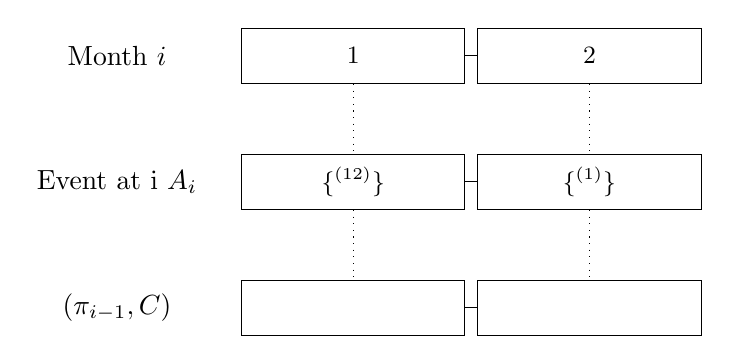
\begin{tikzpicture}[y=1.6cm,x=3.0cm]
    
      \tikzset{
        cell/.style={
          draw, rectangle, text width=26mm,
          minimum height=7mm, align=center, font=\small
        }
      }
    
      % Labels
      \node at (0,0)   {Month $i$};
      \node at (0,-1)  {Event at i $A_i$};
      \node at (0,-2)  {$\Prog(\pi_{i-1},C)$};
      % Row 1: time
      \node[cell] at (1,0) (t1) {$1$};
      \node[cell] at (2,0) (t2) {$2$};
      % Row 2: events
      \node[cell] at (1,-1) (e1) {$\{\PAY^{(12)}\}$};
      \node[cell] at (2,-1) (e2) {$\{\OCC^{(1)}\}$};
      % Row 3: residuals
      \node[cell] at (1,-2) (r1) {\emptc};
      \node[cell] at (2,-2) (r2) {\emptc};
      % Arrows
      \draw (t1)--(t2);
      \draw (e1)--(e2);
      \draw (r1)--(r2);
      % Vertical alignment
      \draw[dotted](t1.south)--(e1.north);
      \draw[dotted](e1.south)--(r1.north);
    
      \draw[dotted](t2.south)--(e2.north);
      \draw[dotted](e2.south)--(r2.north);
    \end{tikzpicture}
    }}
    {Progression on $ \obl[1]{\PAY}\ \repair\ \obl[1]{\PAYF}$ with a trace for which a no reparation is not required}
    {example:prog-repair1}
    {\vspace{8pt}}{\vspace{-12pt}}

\medskip
\noindent\textbf{Scenario 2: Violation and Repair.}
In trace $\pi'$, the tenant fails to pay in Month 1 ($\PAY \notin A'_1$). Here, $\trace{A'_1} \violt \obl[1]{\PAY}$. Consequently, the CPM activates the repair branch. The residual for Month 2 becomes $\obl[1]{\PAYF}$, obliging the tenant to pay the fine.

  \boxalignfigure{\resizebox{0.7\textwidth}{!}{%
  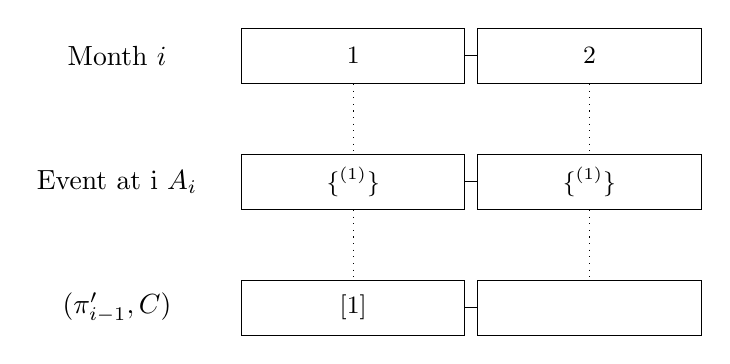
\begin{tikzpicture}[y=1.6cm,x=3.0cm]
  
    \tikzset{
      cell/.style={
        draw, rectangle, text width=26mm,
        minimum height=7mm, align=center, font=\small
      }
    }
  
    % Labels
    \node at (0,0)   {Month $i$};
    \node at (0,-1)  {Event at i $A_i$};
    \node at (0,-2)  {$\Prog(\pi'_{i-1},C)$};
    % Row 1: time
    \node[cell] at (1,0) (t1) {$1$};
    \node[cell] at (2,0) (t2) {$2$};
    % Row 2: events
    \node[cell] at (1,-1) (e1) {$\{\OCC^{(1)}\}$};
    \node[cell] at (2,-1) (e2) {$\{\OCC^{(1)}\}$};
    % Row 3: residuals
    \node[cell] at (1,-2) (r1) {$\obl[1]{\PAYF}$};
    \node[cell] at (2,-2) (r2) {\emptc};
    % Arrows
    \draw (t1)--(t2);
    \draw (e1)--(e2);
    \draw (r1)--(r2);
  
    % Vertical alignment
    \draw[dotted](t1.south)--(e1.north);
    \draw[dotted](e1.south)--(r1.north);
  
    \draw[dotted](t2.south)--(e2.north);
    \draw[dotted](e2.south)--(r2.north);
  
  \end{tikzpicture}
  }}
  {Progression on $ \obl[1]{\PAY}\ \repair\ \obl[1]{\PAYF}$ with a trace for which a no reparation is not required}
  {example:prog-repair2}
  {\vspace{8pt}}{\vspace{-12pt}}
\end{example}

Having established how single-step reparations evolve, we now extend the analysis to ongoing contracts. The following example demonstrates how the CPM handles infinite streams where duties recur every month, showing how violations in one period persist into the next.

\begin{example}[Progression of Infinite Repetition]
Consider the recurring contract $\repit{C_3}$, where the tenant must pay rent (or a fine) every month.
\[ \repit{C_3} = \repit{ \obl[1]{\PAY}\ \repair\ \obl[1]{\PAYF}}. \]

\noindent\textbf{Trace Analysis.}
We observe a trace where the tenant pays in Month 1 but fails to pay in Month 2 (occupying instead).
\begin{itemize}
    \item \textbf{Step 1 ($A_1$):} The tenant pays. The instance of $C_3$ for Month 1 is discharged. Due to the repetition operator, the residual is $\emptc ; \repit{C_3} \equiv \repit{C_3}$. The contract effectively ``resets'' for the next month.
    \item \textbf{Step 2 ($A_2$):} The tenant occupies but does not pay. The instance of $C_3$ for Month 2 is violated. Unlike Step 1, the residual does not reset cleanly. Instead, the violated obligation transforms into its reparation $\obl[1]{\PAYF}$, which must be fulfilled in the \emph{next} step (Month 3), alongside the continuing repetition $\repit{C_3}$.
\end{itemize}
This results in an accumulation of duties: the fine from Month 2 and the new rent for Month 3.

  \boxalignfigure{\resizebox{0.7\textwidth}{!}{%
  \begin{tikzpicture}[y=1.6cm,x=3.0cm]
  
    \tikzset{
      cell/.style={
        draw, rectangle, text width=26mm,
        minimum height=7mm, align=center, font=\small
      }
    }
  
    % Labels
    \node at (0,0)   {Month $i$};
    \node at (0,-1)  {Event at i $A_i$};
    \node at (0,-2)  {$\Prog(\pi_{i-1},C)$};
    % Row 1: time
    \node[cell] at (1,0) (t1) {$1$};
    \node[cell] at (2,0) (t2) {$2$};
    % Row 2: events
    \node[cell] at (1,-1) (e1) {$\{\PAY^{(12)}\}$};
    \node[cell] at (2,-1) (e2) {$\{\OCC^{(1)}\}$};
    % Row 3: residuals
    \node[cell] at (1,-2) (r1) {$\repit{C_3}$};
    \node[cell] at (2,-2) (r2) {$\obl[1]{\PAYF} ; \repit{C_3}$};
    % Arrows
    \draw (t1)--(t2);
    \draw (e1)--(e2);
    \draw (r1)--(r2);
  
    % Vertical alignment
    \draw[dotted](t1.south)--(e1.north);
    \draw[dotted](e1.south)--(r1.north);
  
    \draw[dotted](t2.south)--(e2.north);
    \draw[dotted](e2.south)--(r2.north);
  
  \end{tikzpicture}
  }}
  {Progression on $\repit{C_3}$ where the obligation is met in the first month but violated in the second.}
  {example:prog-repitc1}
  {\vspace{8pt}}{\vspace{-12pt}}
\end{example}

While repetitions capture simple recurring duties, more complex contracts are often bounded by conditions. Finally, we examine how the CPM handles \emph{guarded contracts}, where the outer structure (the guard) and the inner structure (the obligations) evolve independently until a termination event occurs.

\begin{example}[Progression of Guarded Contracts]
We examine a guarded contract that persists until a termination notice ($\notifterm$) is issued.
\[ \guard[\Gamma^+ \cdot \notifterm^{(1)}]{\repit{C_3}} \]

\noindent\textbf{Trace 1: Successful Termination.}
The tenant pays in Month 1 ($A_1$) and issues a termination notice in Month 2 ($A_2$).
\begin{itemize}
    \item At $i=1$, the event $A_1$ satisfies the inner contract $C_3$ (rent paid), but does not satisfy the guard (no notice). The residual is the guarded repetition.
    \item At $i=2$, the event $A_2$ contains $\notifterm$. This satisfies the guard expression. The CPM immediately reduces the entire contract to $\emptc$, signifying the contract has ended.
\end{itemize}

  \boxalignfigure{\resizebox{0.85\textwidth}{!}{%
  \begin{tikzpicture}[y=1.8cm,x=3.8cm]
  
    \tikzset{
      cell/.style={
        draw, rectangle, text width=34mm,
        minimum height=8mm, align=center, font=\small
      }
    }
    % Local definition for the residual regex to fit in the box
    \def\resid{\notifterm \mid \Gamma^+ \cdot \notifterm}
  
    % Labels
    \node at (0,0)   {Month $i$};
    \node at (0,-1)  {Event at i $A_i$};
    \node at (0,-2)  {$\Prog(\pi_{i-1},C)$};
    % Row 1: time
    \node[cell] at (1,0) (t1) {$1$};
    \node[cell] at (2,0) (t2) {$2$};
    % Row 2: events
    \node[cell] at (1,-1) (e1) {$\{\PAY^{(1)}, \PAY^{(2)}\}$};
    \node[cell] at (2,-1) (e2) {$\{\OCC^{(1)}, \notifterm^{(1)}\}$};
    % Row 3: residuals
    % Step 1: Contract satisfied (payment made), Guard not satisfied yet (needs >0 length or specific event).
    % Residual guard becomes (Notif | Gamma+ . Notif)
    \node[cell] at (1,-2) (r1) {$\guard[\resid]{\repit{C_3}}$};
    % Step 2: Guard satisfied by NotifTerm in A2. Contract discharges to epsilon.
    \node[cell] at (2,-2) (r2) {\emptc};
    % Arrows
    \draw (t1)--(t2);
    \draw (e1)--(e2);
    \draw (r1)--(r2);
  
    % Vertical alignment
    \draw[dotted](t1.south)--(e1.north);
    \draw[dotted](e1.south)--(r1.north);
  
    \draw[dotted](t2.south)--(e2.north);
    \draw[dotted](e2.south)--(r2.north);
  
  \end{tikzpicture}
  }}
  {Progression on guarded contract where the termination notice at step 2 discharges the contract.}
  {example:prog-guard1}
  {\vspace{8pt}}{\vspace{-12pt}}

\medskip
\noindent\textbf{Trace 2: Pending Guard with Internal Violation.}
In this scenario, the tenant pays in Month 1 but fails to pay (and gives no notice) in Month 2.
\begin{itemize}
    \item At $i=2$, the guard is \emph{not} satisfied.
    \item Simultaneously, the inner contract $\repit{C_3}$ processes the event. Since rent was not paid, the inner contract evolves into a reparation state ($\obl[1]{\PAYF}$).
    \item The resulting residual is a guarded reparation: $\guard[\dots]{(\obl[1]{\PAYF} ; \repit{C_3})}$.
\end{itemize}
This illustrates how the CPM maintains the ``wrapper'' (the guard) while the content inside (the obligations) evolves and accumulates violations independently.

  \boxalignfigure{\resizebox{0.95\textwidth}{!}{%
  \begin{tikzpicture}[y=1.8cm,x=4.4cm]
  
    \tikzset{
      cell/.style={
        draw, rectangle, text width=40mm,
        minimum height=8mm, align=center, font=\small
      }
    }
    \def\resid{\notifterm \mid \Gamma^+ \cdot \notifterm}
  
    % Labels
    \node at (0,0)   {Month $i$};
    \node at (0,-1)  {Event at i $A_i$};
    \node at (0,-2)  {$\Prog(\pi'_{i-1},C)$};
    
    % Row 1: time
    \node[cell] at (1,0) (t1) {$1$};
    \node[cell] at (2,0) (t2) {$2$};
    
    % Row 2: events
    \node[cell] at (1,-1) (e1) {$\{\PAY^{(1)}, \PAY^{(2)}\}$};
    \node[cell] at (2,-1) (e2) {$\{\OCC^{(1)}\}$};
    
    % Row 3: residuals
    % Step 1: Manual line break using \\
    \node[cell] at (1,-2) (r1) {$\lceil \resid \rceil$ \\ $\repit{C_3}$};
    % Step 2: Manual line break using \\
    \node[cell] at (2,-2) (r2) {$\lceil \resid \rceil$ \\ $(\obl[1]{\PAYF} ; \repit{C_3})$};
    % Arrows
    \draw (t1)--(t2);
    \draw (e1)--(e2);
    \draw (r1)--(r2);
  
    % Vertical alignment
    \draw[dotted](t1.south)--(e1.north);
    \draw[dotted](e1.south)--(r1.north);
  
    \draw[dotted](t2.south)--(e2.north);
    \draw[dotted](e2.south)--(r2.north);
  
  \end{tikzpicture}
  }}
  {Progression on guarded contract where the guard is not satisfied and the inner contract triggers a reparation.}
  {example:prog-guard2}
  {\vspace{8pt}}{\vspace{-12pt}}
  
\end{example}


\section{Quantative violation semantics}
To define the quantitative violation semantics to not stop at the first violation prefix, we reuse  \emph{Contract Progress function} as the underlying state-transition mechanism.
 The progression function $\Prog$ is utilized to dynamically evolve the contract after every observation, producing a sequence of \emph{residual contracts} that represent the exact normative state at each point in time.
  By updating the contract state step-by-step, we ensure that the violation score for any given event is calculated strictly against the specific literals in force at that moment, accounting for all prior satisfactions, discharges, or triggered reparations. Then propagating the updated residual to the subsequent evaluation step.
  \begin{definition}[Quantitative Violation Semantics]
    Let $\trace{A}$ be a single event trace over $\Gamma$,  $\pi$ be a (possibly empty) finite trace $\Gamma^*$, and $C$ be a contract from $\cDL$.
    We define the \emph{quantitative violation semantics}, denoted by $\qsem{}: \Gamma^*, \cDL \to \mathbb{N} $, which maps a trace and a contract to a  natural number representing the violation score of trace on the contract. 
    The function is defined recursively by evaluating the head of the trace ($\trace{A}$) and propagating the residual contract to the tail ($\pi$):
    \[
    \qsem{\trace{A}\concat \pi, C} :=
    \begin{cases} 
      \qsem{\trace{A}, C } & \text{if } \pi = \epsilon \lor \Prog(\trace{A},C)= \emptc,\\
      \qsem{\trace{A}, C } + \qsem{\pi, \Prog(\trace{A},C)} & \text{otherwise}.
    \end{cases}
    \]
    where the \emph{instantaneous violation score} for a single event $\trace{A}$ against a contract $C$ is defined inductively on the structure of the contract:
    \[
    \qsem{\trace{A}, C} :=
    \begin{cases} 
      \qsem{\trace{A}, C_1 } + \qsem{\trace{A}, C_2} & \text{if } C = C_1 \wedge C_2, \\
      1 & \text{if } \trace{A} \violt C, \\
      0 & \text{otherwise}.
    \end{cases}
    \]
    \end{definition}
Intuitively, the formula $\qsem{\trace{A}\concat \pi, C}$ treats the contract execution as a path-accumulation problem. At every time step, the function:
\begin{enumerate}
    \item \textbf{Snapshots the penalty:} It calculates $\qsem{\trace{A}, C}$, which asks ``Given the current literals from$C$, does the current event $A$ violate any of them?'' This is a stateless check based purely on the structure of $C$ at that instant.
    \item \textbf{Updates the state:} It computes $\Prog(\trace{A}, C)$, effectively moving the contract pointer forward (e.g., from a paid obligation to the next month's rent, or from a violated duty to a reparation).
    \item \textbf{Accumulates:} It adds the snapshot penalty to the result of the recursive call on the remaining trace using the \emph{new} state.
\end{enumerate}

Intuitively, the formula $\qsem{\trace{A}\concat \pi, C}$ treats the contract execution as a path-accumulation problem. At every time step, the function:
\begin{enumerate}
    \item \textbf{Snapshots the penalty:} It calculates $\qsem{\trace{A}, C}$, which asks ``Given the current literals from $C$, does the current event $A$ violate any of them?'' This is a stateless check based purely on the structure of $C$ at that instant.
    \item \textbf{Updates the state:} It computes $\Prog(\trace{A}, C)$, effectively moving the contract pointer forward (e.g., from a paid obligation to the next month's rent, or from a violated duty to a reparation).
    \item \textbf{Accumulates:} It adds the snapshot penalty to the result of the recursive call on the remaining trace using the \emph{new} state.
\end{enumerate}

The explicit handling of Sequence and Reparation is done in the contract progress function, which ensures that ``zero-delay'' transitions are penalized correctly. For instance, if a contract requires $C_1$ then $C_2$, and an event discharges $C_1$ but violates $C_2$ in the same step, the summation logic ($\qsem{\trace{A}, C_1} + \qsem{\trace{A}, C_2}$) ensures the violation of $C_2$ is not ignored simply because it appeared in a continuation.


The definition of the instantaneous score $\qsem{\trace{A}, C}$ rests on distinguishing between \textbf{concurrent} (parallel) obligations and \textbf{structural} (atomic) constraints. It decouples the measurement of the ``volume'' of non-compliance from the binary verification of specific rules.

\paragraph{Additivity of Concurrency.}
The case $\qsem{\trace{A}, C_1 \wedge C_2} := \qsem{\trace{A}, C_1 } + \qsem{\trace{A}, C_2}$ captures the ``width'' of the violation as show in Example.\ref{fig:joint-blame}. In normative systems, a conjunction represents distinct, independent obligations active simultaneously. By summing the scores, the function ensures that the penalty is proportional to the number of distinct parallel duties neglected in a single instant, preventing ``violation masking'' where a single boolean verdict would hide multiple breaches.

\paragraph{Binary Structural Verdict.}
For constructs that are not distinct parallel duties (such as literals, sequences, or reparations), the definition relies on the binary tight violation relation ($\violt$). This captures the ``existence'' of a fault in a non-decomposable structure. For example, a single atomic duty ($\obl{a}$) can only be violated once per step.

\paragraph{Separation of State and Score.}
This approach assumes that the complexity of temporal evolution is handled by $\Prog$, while $\qsem{}$ handles the instantaneous cost. By reducing non-conjunction cases to a simple check ($\trace{A} \violt C$), the definition asserts that scoring is local (checking if the current active node is broken), while progression is temporal (handling the flow from one obligation to the next).

We summarize these properties in the following theorem, which establishes that the quantitative score is a monotonically increasing function that acts as a "super-set" of the binary violation semantics.
While a binary trace might be "Satisfied" (via reparation), the quantitative score reveals the cost of that path.

\subsection{Formal Correspondence between Tight and Quantitative Semantics}

The quantitative semantics presented above is not an arbitrary metric but a consistent extension of the forward-looking tight semantics.
While tight semantics provides a binary decisive verdict (satisfaction vs.\ violation), the quantitative semantics provides a cumulative measure of deviation.
We now establish the formal link between these two frameworks through the properties of \emph{Score Stability} and \emph{Violation Detection}.

The first connection concerns the relationship between the discharge of a contract (reaching $\emptc$) and the tight satisfaction relation $\satt$.
When a contract is tightly satisfied, it conceptually ceases to impose new requirements.
The progression function reflects this by transitioning to the neutral element $\emptc$.

\begin{lemma}[Satisfaction Saturation]
\label{lem:sat-saturation}
Let $C$ be a contract and $\pi$ be a finite trace.
If the contract is tightly satisfied by $\pi$, the progression function reduces to the empty contract, and the cumulative violation score stabilizes.
Formally:
\[
\pi \satt C \implies \Prog(\pi, C) = \emptc.
\]
Consequently, for any extension $\pi'$ of $\pi$:
\[
\qsem{\pi \concat \pi', C} = \qsem{\pi, C}.
\]
\end{lemma}

\begin{proof}
The proof follows from the definition of $\Prog$.
For every construct (Literal, Reparation, Guard, Trigger), the progression function is defined to return $\emptc$ exactly when the condition $\trace{A} \satt C$ is met.
Since $\qsem{\trace{A}, \emptc} = 0$ for any event $A$, no further penalties can be accumulated once the residual contract becomes $\emptc$.
\end{proof}

The second connection concerns the relationship between tight violations and the instantaneous score.
A key feature of the quantitative semantics is that it is strictly stricter than the binary semantics: it assigns a positive penalty to \emph{every} tight violation, even those that are subsequently repaired.

\begin{lemma}[Positive Penalty for Tight Violation]
\label{lem:violation-penalty}
Let $C$ be a contract and $\trace{A}$ be a single event.
If the event tightly violates the contract, the instantaneous violation score is strictly positive.
\[
\trace{A} \violt C \implies \qsem{\trace{A}, C} \ge 1.
\]
\end{lemma}

\begin{proof}
We proceed by structural induction on $C$.
\begin{itemize}
    \item \textbf{Base Case (Literals):} If $\trace{A} \violt \ell$, then by definition $\qsem{\trace{A}, \ell} = 1$.
    \item \textbf{Conjunction ($C_1 \wedge C_2$):} By Definition~\ref{def:binary-contract-semantics}, $\trace{A} \violt C_1 \wedge C_2$ implies $\trace{A} \violt C_1$ or $\trace{A} \violt C_2$.
    Consequently, $\qsem{\trace{A}, C_1} \ge 1$ or $\qsem{\trace{A}, C_2} \ge 1$. Since the score is additive ($\qsem{\trace{A}, C_1} + \qsem{\trace{A}, C_2}$), the total is $\ge 1$.
    \item \textbf{Reparation ($C_1 \repair C_2$):} $\trace{A} \violt C_1 \repair C_2$ implies $\trace{A} \violt C_1$ and $\trace{A} \violt C_2$.
    The scoring function sums violations of $C_1$ (score 1) and $C_2$. Thus, the score is at least 1.
\end{itemize}
The sequence case follows similarly via the immediate handover logic.
\end{proof}

We summarize these properties in the following theorem, which establishes that the quantitative score is a monotonically increasing function that acts as a "super-set" of the binary violation semantics.
While a binary trace might be "Satisfied" (via reparation), the quantitative score reveals the cost of that path.


\begin{theorem}[Consistency of Quantitative and Tight Semantics]
  \label{thm:quant-consistency}
  For any contract $C$ and finite trace $\pi$:
  \begin{enumerate}
      \item \textbf{Zero Score Implications:}
      If $\qsem{\pi, C} = 0$, then exactly one of the following three disjoint cases holds:
      \begin{enumerate}
        \item $\pi \satt C$ if and only if $\Prog(\pi, C) = \emptc$ and $\forall k < |\pi|-1:\Prog(\pi[0,k], C) \neq \emptc$.
        \item $\pi \postsat C$ if and only if $\Prog(\pi, C) = \emptc$ and\\ $\exists k < |\pi|-1$ such that $\Prog(\pi[0,k], C) = \emptc$.
        \item $\pi \presat C$ if and only if $\Prog(\pi, C) \neq \emptc$.
      \end{enumerate}
      
      \item \textbf{Non-Zero Score Implications:}
      If $\qsem{\pi, C} \neq 0$, then:
      \begin{enumerate}
        \item $\pi \violt C$ if and only if $\qsem{\pi, C} = 1$ and $\qsem{\pi[0, |\pi|-2], C} = 0$.
        \item $\pi \postviol C$ if and only if $\qsem{\pi, C} > 1$ or ($\qsem{\pi, C} = 1$ and\\ $\qsem{\pi[0, |\pi|-2], C} = 1$).
      \end{enumerate}
      
      \item \textbf{Reparation Cost:}
      If $\pi$ satisfies $C$ strictly through a reparation mechanism (i.e., $\pi \satt C$ but primary obligations failed), then $\qsem{\pi, C} > 0$.
  \end{enumerate}
  \end{theorem}
  
  \begin{proof}
  We prove the implications by structural induction on the trace $\pi$ and the contract $C$, utilizing the definitions of the quantitative function $\qsem{}$ and the contract progression $\Prog$.
  
  \paragraph{1. Zero Score Implications ($\qsem{\pi, C} = 0$)}
  Assume $\qsem{\pi, C} = 0$. By the definition of the cumulative score, this implies that for all steps $i < |\pi|$, the instantaneous penalty is zero: $\qsem(\trace{A_i}, C_i) = 0$. Consequently, no tight violation has occurred at any step. The contract state evolves purely via $\Prog$ without triggering any penalty clauses.
  
  \begin{enumerate}
      \item \textbf{Case 1(a): Tight Satisfaction ($\satt$).}
      \begin{itemize}
          \item $(\Rightarrow)$ Assume $\Prog(\pi, C) = \emptc$ and for all strict prefixes $\pi'$, $\Prog(\pi', C) \neq \emptc$.
          The condition $\Prog(\pi, C) = \emptc$ indicates that the contract has been fully discharged. Since the score is 0, this discharge was not achieved via a violation-triggered path (e.g., a reparation where the primary failed). The absence of $\emptc$ in prior prefixes ensures that this is the \emph{first} moment of discharge. By Definition~\ref{def:binary-contract-semantics} (Tight Satisfaction), the first prefix to fully satisfy the obligations corresponds to $\satt$.
          \item $(\Leftarrow)$ If $\pi \satt C$, then by Lemma~\ref{lem:sat-saturation} (Satisfaction Saturation), the progression must reach $\emptc$ exactly at $\pi$. Since it is a \emph{tight} satisfaction, no proper prefix could have satisfied it (reached $\emptc$) earlier.
      \end{itemize}
  
      \item \textbf{Case 1(b): Post Satisfaction ($\postsat$).}
      \begin{itemize}
          \item The condition $\exists k < |\pi|$ such that $\Prog(\pi[0,k], C) = \emptc$ implies that the contract was already discharged at a previous step $k$.
          \item By Definition~\ref{def:postprecont}, $\pi \postsat C$ holds if there exists a strict prefix that tightly satisfies $C$. Since the score is 0, the path to $k$ was compliant. Thus, the state remains $\emptc$ for the remainder of the trace, maintaining the $\postsat$ status.
      \end{itemize}
  
      \item \textbf{Case 1(c): Pre Satisfaction ($\presat$).}
      \begin{itemize}
          \item Assume $\Prog(\pi, C) \neq \emptc$. Since $\qsem{\pi, C} = 0$, no violation has occurred. However, the contract has not reduced to the empty contract $\emptc$, meaning active obligations remain.
          \item This satisfies the definition of $\presat$: the trace is neither satisfied ($\satt/\postsat$) nor violated ($\violt/\postviol$). It is effectively "pending."
      \end{itemize}
  \end{enumerate}
  
  \paragraph{2. Non-Zero Score Implications ($\qsem{\pi, C} \neq 0$)}
  Assume $\qsem{\pi, C} > 0$. This implies $\exists i$ such that $\qsem(\trace{A_i}, C_i) > 0$.
  
  \begin{enumerate}
      \item \textbf{Case 2(a): Tight Violation ($\violt$).}
      \begin{itemize}
          \item We consider the case where $\qsem{\pi, C} = 1$, the score of the immediate prefix is $0$ and let $n= \size{\pi}$ .
          \item $\qsem{\pi[0..n-2], C} = 0$ implies that for all previous steps, the contract was in a compliant state ($\presat$).
          \item The jump to $\qsem{\pi, C} = 1$ implies that the instantaneous score at the last step $\qsem{\trace{A_{n-1}}, \Prog(\pi[0,n-2],C)} = 1$.
          \item By Lemma~\ref{lem:violation-penalty}, a positive instantaneous score corresponds to a tight violation of the active residual contract.
          \item Since this is the \emph{first} non-zero score, it corresponds to the \emph{first} prefix that triggers a violation. This matches the definition of $\pi \violt C$.
      \end{itemize}
  
      \item \textbf{Case 2(b): Post Violation ($\postviol$).}
      \begin{itemize}
          \item The condition $\qsem{\pi, C} > 1$ or ($\qsem{\pi, C}=1$ and $\qsem{prefix}=1$) implies that the violation score did not originate purely at the current step (or if it did, it was cumulative).
          \item Specifically, if $\qsem{\pi[0..n-2], C} \ge 1$, then a violation occurred strictly in the past.
          \item By Definition~\ref{def:postprecont}, if a strict prefix tightly violated the contract ($\violt$), the current trace is in $\postviol$. The non-zero score is carried forward monotonically.
      \end{itemize}
  
      \item \textbf{Case 2(c): Reparation Cost.}
      \begin{itemize}
          \item Consider a contract $C_{primary} \repair C_{repair}$.
          \item If $\pi$ satisfies this strictly through the reparation mechanism, it means $\pi$ did \emph{not} satisfy $C_{primary}$.
          \item By the definition of reparation progression, the transition to $C_{repair}$ occurs only if $\pi \violt C_{primary}$.
          \item By the definition of the instantaneous scoring function for reparation,\\ $\qsem{\trace{A}, C_{primary} \repair C_{repair}} = 1 + \dots$ when the primary violates.
      \end{itemize}
      Therefore, the path involving the repair accumulates a score of at least 1 (the penalty for breaking the primary), confirming $\qsem{\pi, C} > 0$.
  \end{enumerate}
  \end{proof}

This theorem highlights the utility of the quantitative approach for post-hoc analysis: distinguishing between a "perfect" execution (Score 0) and a "compliant but costly" execution (Score $>0$, e.g., paying fines), a distinction lost in the binary $\satt$ verdict.